%!TEX root = ../thesis.tex
%*******************************************************************************
%****************************** Second Chapter **********************************
%*******************************************************************************
\chapter{LAG SIM: A versatile, user-friendly structured illumination microscope} \label{chap:LAGSIM}

% **************************** Define Graphics Path **************************
\ifpdf
    \graphicspath{{Chapter2/Figs/Raster/}{Chapter2/Figs/PDF/}{Chapter2/Figs/}}
\else
    \graphicspath{{Chapter2/Figs/Vector/}{Chapter2/Figs/}}
\fi

%``The LAG SIM works good now and I really love it!''
%
%\textit{Email from Meng Lu (Molecular Neuroscience Group, Cambridge), 26-06-2018}

\section{Introduction} \label{sec:simintro}
\subsection{Background to SIM} \label{sec:sim-background}
Widefield epifluorescent microscopes use a uniform field of light to illuminate a labelled sample~\cite[\textit{ch. 2}]{lakowicz2007principles}.
Fluorescent emission light is then emitted from any fluorescent molecule located within the microscope's field of view~\cite{pawley2012handbook}.
In this type of microscope, fluorescent molecules above and below the focal plane of the lens will also receive illumination light and fluoresce, causing an out-of-focus blur on the image~\cite{wilson1984theory}.

Out-of-focus light can be removed by placing a pinhole in the excitation and emission path, and scanning the small spot of light across the sample to build up an image one pixel at a time.
This technique, invented in 1955 and called confocal microscopy, physically blocks out-of-focus light, making 3D reconstructions of samples possible~\cite{marvin1961microscopy}.
The cost of this optical sectioning is a slow acquisition speed due to the nature of a point-scanning technique.

A faster way of removing out-of-focus light can be achieved with total internal reflection fluorescence (TIRF)~\cite[\textit{ch. 21}]{periasamy2013methods}.
In this scheme light is projected into the outer edge of the back-aperture of a specialised lens, such that it emerges from the lens steeper than the critical angle required for reflection, rather than refraction, from a glass interface.
Although this means that no light passes through the microscope slide, as shown in Figure~\ref{fig:tirf-illumination}, energy from the evanescent field is able to couple into molecules close to the coverglass, inducing fluorescence~\cite{axelrod1981cell}.
TIRF illuminates molecules within \SI{100}{\nano\metre} of the coverglass without obscuration by out-of-focus light, with the disadvantage that details deeper into the sample cannot be observed.

\begin{figure}[tbp]
\centering
\begin{subfigure}[b]{0.49\textwidth}
	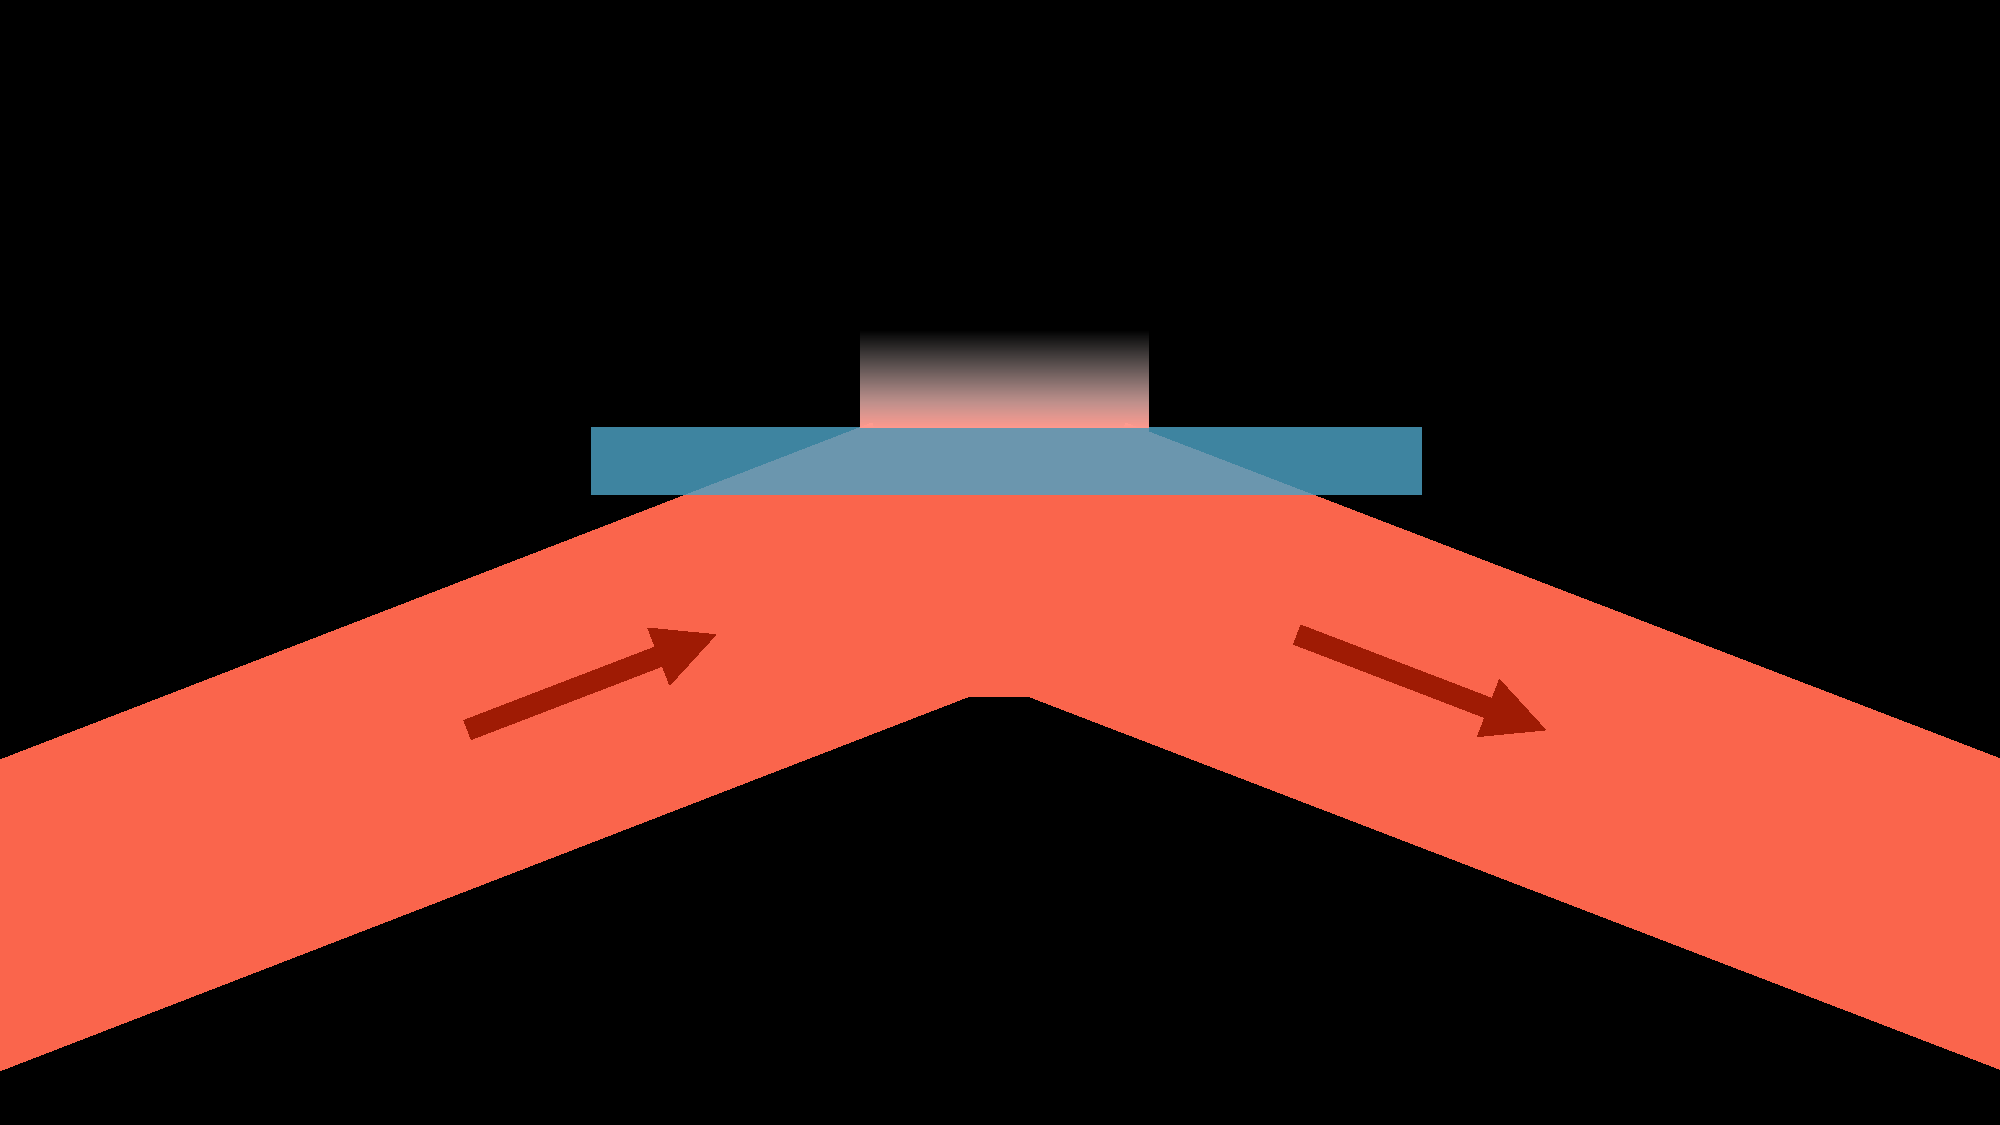
\includegraphics[width=\textwidth]{tirf-illumination}
	\caption{}\label{fig:tirf-illumination}
\end{subfigure}
\hfill
\begin{subfigure}[b]{0.49\textwidth}
	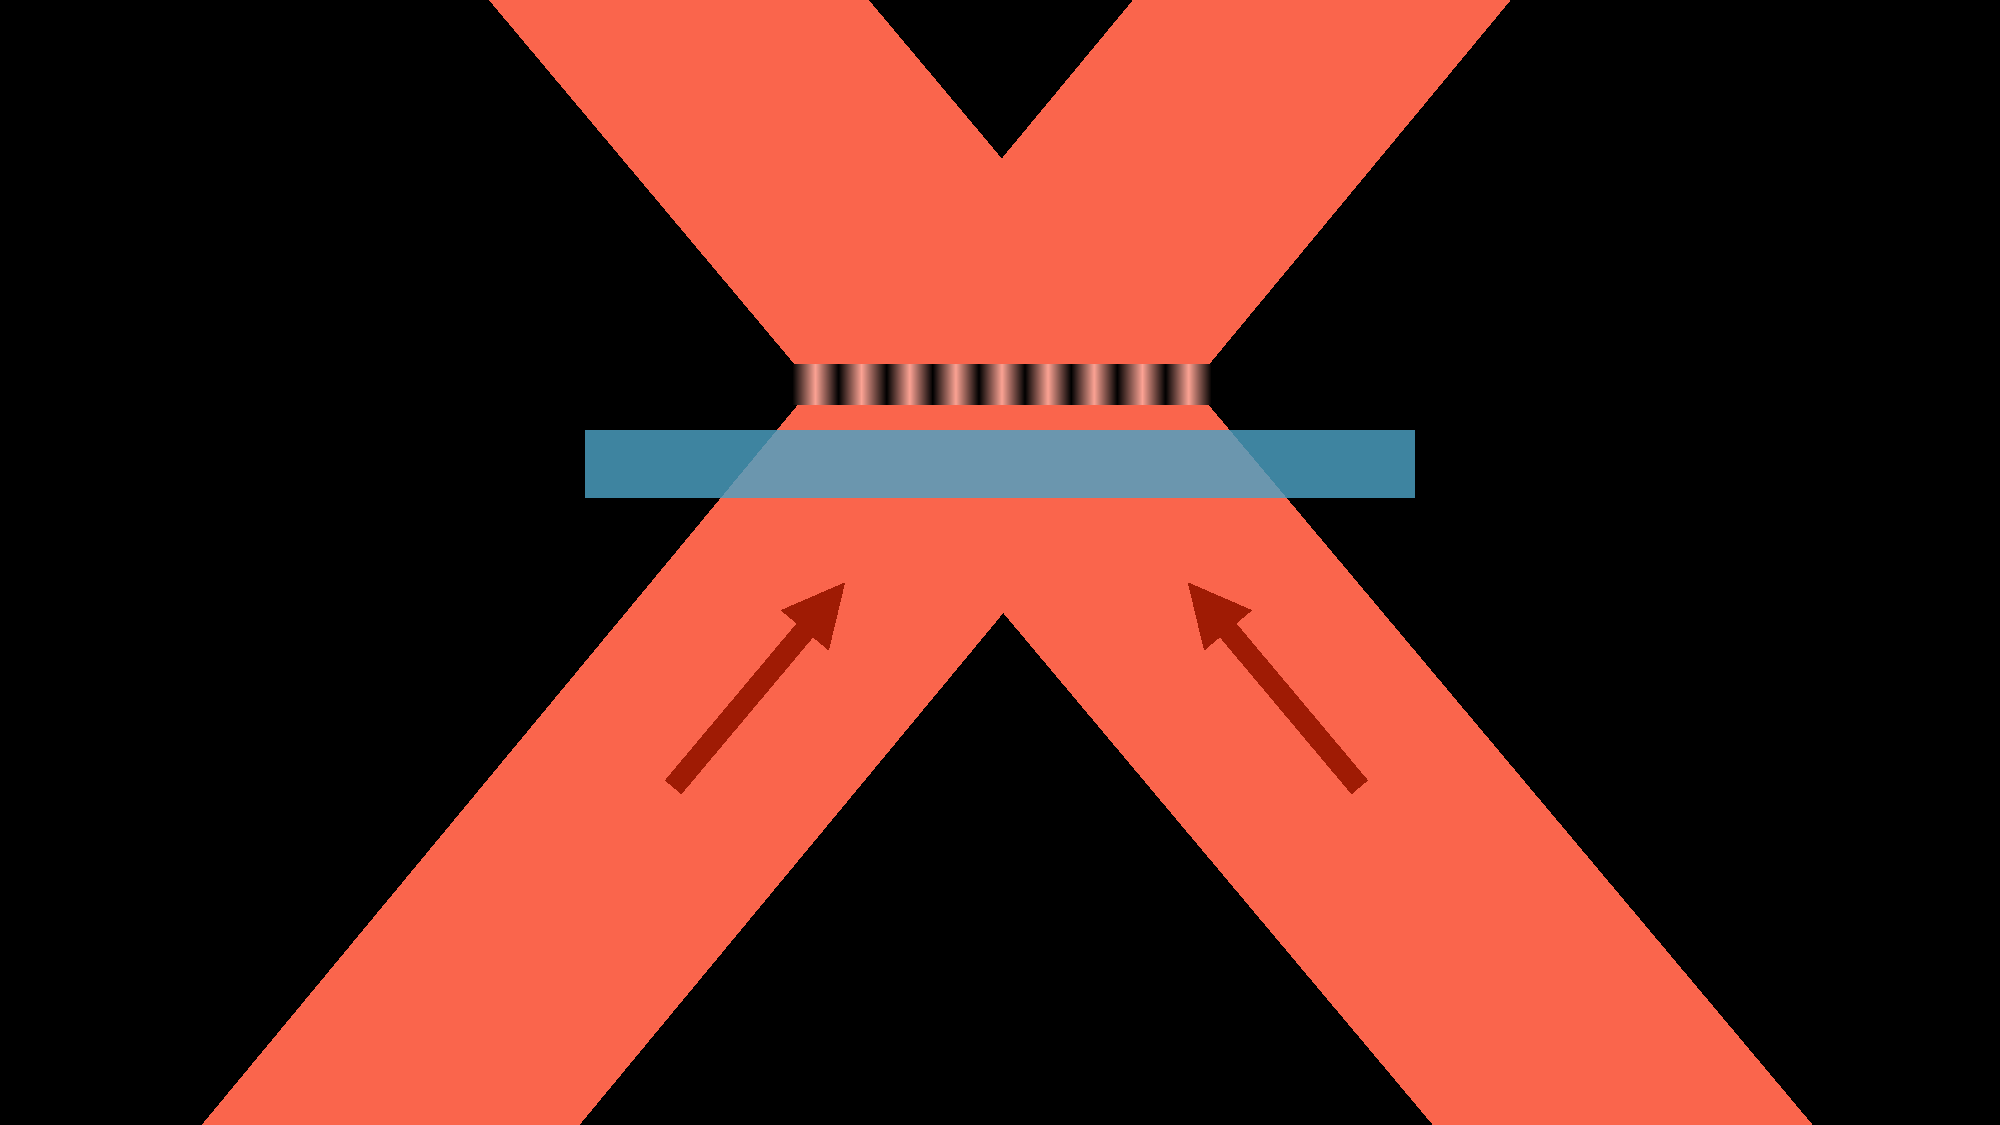
\includegraphics[width=\textwidth]{os-illumination}
	\caption{}\label{fig:os-illumination}
\end{subfigure}
\caption[LAG SIM: Both TIRF microscopy and structured illumination patterns can be used to remove out-of-focus light]{(a) shows a TIRF illumination scheme, where light intercepts the cover glass at an angle steeper than the critical angle for total internal reflection. The evanescent wave created can excite fluorphores in the closest \SI{100}{\nano\metre} to the coverglass, decaying exponentially in intensity. (b) shows the generation of a structured illumination pattern by the interference of two beams. This can be used to computationally reconstruct an optically sectioned image, as shown in Figure~\ref{fig:os-sim-comparison}. Diagrams are not to scale. }
\label{fig:os-sim-comparison}
\end{figure}

Sheppard and Wilson showed that optical sectioning can be achieved computationally if the illumination light is modulated with a structured pattern~\cite{pawley2012handbook, neil1997method}.
Sinusoidal illumination can be produced by two coherent beams of light generated by a binary grating, which interfere at the focal plane of the objective lens as shown in Figure~\ref{fig:os-illumination}.
The resulting image $I$ is described by Equation~\ref{eq:wilson-illumination}, where $W$ is the equivalent widefield image without structured illumination, $m$ the modulation depth, $t$ the modulation frequency, and $x$ a lateral spatial dimension in the sample plane.

\begin{equation} \label{eq:wilson-illumination}
I_i = W \left( 1 + m \cos \left(t x + \phi_i \right) \right)
\end{equation}

Since the sinusoidal illumination pattern is only generated in the focal plane of the objective lens, extracting the $Wm$ component from Equation~\ref{eq:wilson-illumination} constructs an image $I_R$ in which the unmodulated out-of-focus light has been removed.
Proofs~\ref{pro:square} and \ref{pro:homo} show that this requires the illumination to be stepped through three equally-spaced phases $\phi_i = \left\lbrace0, \frac{2\pi}{3}, \frac{4\pi}{3}\right\rbrace$, with an image $I_i$ captured at each step $i=\left\lbrace1,2,3\right\rbrace$.
The proofs verify that either the square law detection of Equation~\ref{eq:wilson-square-law} or the homodyne detection shown in Equation~\ref{eq:wilson-homodyne} can be used to extract just the $Wm$ term~\cite{neil1997method}, multiplied in each case by a constant scaling factor.

If the acquired images are simply summed together, the result $I_1+I_2+I_3$ is $W$, the image that would be obtained from a widefield microscope.
Figure~\ref{fig:os-sim-widefield} shows this sum for an image of the Herpes Simplex Virus Type 1 (HSV-1) infecting a human foreskin fibroblast (HFF) cell.
When the raw images $I_i$ are reconstructed with the square-law detection of Equation~\ref{eq:wilson-square-law}, however, Figure~\ref{fig:os-sim} shows the effective removal of out-of-focus light.

\begin{proof}
\caption{Square law detection removes out-of-focus light from 3 SIM images.}\label{pro:square}

\begin{equation*}
I_1 = W(1+m\cos(tx)),~I_2 = W(1+m\cos(tx+\frac{2\pi}{3})),~I_3 = W(1+m\cos(tx-\frac{2\pi}{3}))
\end{equation*}
\begin{equation*}
I_r^2 = (I_1 - I_2)^2 + (I_1 - I_3)^2 + (I_2 - I_3)^2
\end{equation*}
\textit{Substitute $I_1$, $I_2$, and $I_3$ into the expression for $I_r^2$:}

\begin{align*}
=W^2m^2\Bigg(\left(\cos(tx)-\cos(tx+\frac{2\pi}{3})\right)^2+&\left(\cos(tx)-\cos(tx-\frac{2\pi}{3})\right)^2\\&+\left(\cos(tx+\frac{2\pi}{3})-\cos(tx-\frac{2\pi}{3})\right)^2\Bigg)
\end{align*}

\textit{Expand squared brackets:}

\begin{align*}
=& W^2m^2\Big(2\cos^2(tx) + 2\cos^2(tx+\frac{2\pi}{3}) + 2\cos^2(tx-\frac{2\pi}{3})
 \\& - 2\cos(tx)\cos(tx+\frac{2\pi}{3}) - 2\cos(tx)\cos(tx-\frac{2\pi}{3}) - 2\cos(tx+\frac{2\pi}{3})\cos(tx-\frac{2\pi}{3})\Big)
\end{align*}

\textit{Apply double angle formulae to $\cos^2$ and $\cos(A)\cos(B)$ terms:}

\begin{align*}
= W^2m^2\Big(3 + \cos(2tx) &+ \cos(2tx+\frac{4\pi}{3}) + \cos(2tx-\frac{4\pi}{3})
- \cos(2tx+\frac{2\pi}{3}) \\&- \cos(-\frac{2\pi}{3}) - \cos(2tx-\frac{2\pi}{3}) - \cos(\frac{2\pi}{3}) -\cos(2tx) - cos(0)\Big)
\end{align*}

\textit{Note that $\cos(x+\phi) = \cos(x+2\pi n\phi)$, $n\in \mathbb{Z}$:}

\begin{align*}
= W^2m^2(3 + 0.5 + 0.5 - 1)
\end{align*}
\begin{align*}
= 3W^2m^2
\end{align*}

\textit{Take square root:}

\begin{align*}
I_r = \sqrt3Wm
\end{align*}

\end{proof}

\begin{proof}
\caption{Homodyne detection removes out-of-focus light from 3 SIM images. This gives the same result as square-law detection, albeit a different scaling factor. }\label{pro:homo}

\begin{equation*}
I_1 = W(1+m\cos(tx)),~I_2 = W(1+m\cos(tx+\frac{2\pi}{3})),~I_3 = W(1+m\cos(tx-\frac{2\pi}{3}))
\end{equation*}
\begin{equation*}
I_r = \abs{I_1 + I_2 \exp\left(\frac{2\pi j}{3}\right) + I_3 \exp\left(-\frac{2\pi j}{3}\right)}
\end{equation*}

\textit{Substitute $I_1$, $I_2$, and $I_3$ into the expression for $I_r$:}

\begin{align*}
= W &\abs{(1 + \exp\left(\frac{2\pi j}{3}\right) + \exp\left(-\frac{2\pi j}{3}\right)} \\
& + Wm \abs{\left(\cos(tx) + \cos(tx+\frac{2\pi}{3})(-0.5 + \frac{\sqrt3j}{2}) + \cos(tx-\frac{2\pi}{3})(-0.5 - \frac{\sqrt3j}{2}) \right)}
\end{align*}

\textit{Note that $\abs{(1 + \exp\left(\frac{2\pi j}{3}\right) + \exp\left(-\frac{2\pi j}{3}\right)}=0$:}

\begin{align*}
= Wm \abs{\left(\cos(tx) + \cos(tx+\frac{2\pi}{3})(-0.5 + \frac{\sqrt3j}{2}) + \cos(tx-\frac{2\pi}{3})(-0.5 - \frac{\sqrt3j}{2}) \right)}
\end{align*}

\textit{Gather real and imaginary terms:}

\begin{align*}
= Wm \Bigg\lvert\cos(tx) - &0.5\left(\cos(tx+\frac{2\pi}{3})+(\cos(tx-\frac{2\pi}{3})\right) \\ &+ \frac{\sqrt3j}{2}\left(\cos(tx+\frac{2\pi}{3})-(\cos(tx-\frac{2\pi}{3})\right)\Bigg\rvert
\end{align*}

\textit{Apply double angle formulae for $2\cos(A)\cos(B)$ and $2\sin(A)\sin(B)$:}

\begin{equation*}
= Wm \abs{\cos(tx) - \left(\cos(tx)\cos(\frac{2\pi}{3})\right) + \sqrt3j\left(\cos(tx)\cos(\frac{2\pi}{3})\right)}
\end{equation*}
\begin{equation*}
= Wm \abs{\cos(tx) + 0.5\cos(tx) - \frac{3j}{2}\sin(tx)}
\end{equation*}
\begin{equation*}
= \frac{3}{2}Wm \abs{\cos(tx)-j\sin(tx)}
\end{equation*}
\begin{equation*}
I_r = \frac{3}{2}Wm
\end{equation*}
\end{proof}

\begin{figure}[tb]
\centering
\begin{subfigure}[b]{0.49\textwidth}
	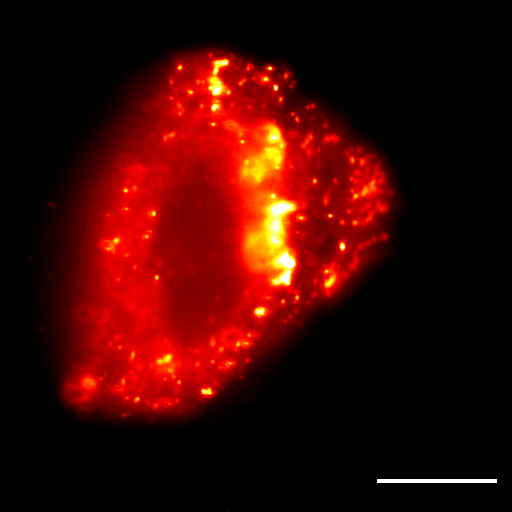
\includegraphics[width=\textwidth]{os-sim-widefield}
	\caption{}\label{fig:os-sim-widefield}
\end{subfigure}
\hfill
\begin{subfigure}[b]{0.49\textwidth}
	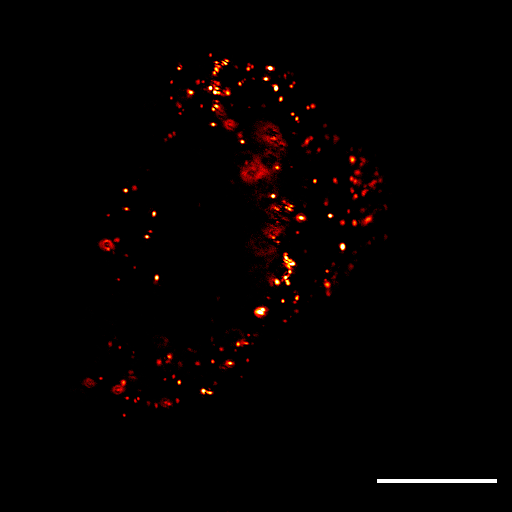
\includegraphics[width=\textwidth]{os-simd}
	\caption{}\label{fig:os-sim}
\end{subfigure}
\caption[LAG SIM: Structured illumination can be used to computationally remove out-of-focus light]{(a) shows a widefield image, $W$, of HSV-1 infecting a human foreskin fibroblast (HFF) cell. (b) shows the same image after illumination with 3 phase-stepped sinusoidal patterns, which are only generated at the focal plane of the objective lens. Combining the images with square-law detection shown in Equation~\ref{eq:wilson-square-law} leaves just the $Wm$ term derived in Proofs~\ref{pro:square} and \ref{pro:homo}, effectively removing the out-of-focus light. Human foreskin fibroblast (HFF) cells were prepared and infected by Katharina Scherer. Scalebar is \SI{10}{\micro\metre}. }
\label{fig:os-sim-comparison}
\end{figure}

\begin{equation} \label{eq:wilson-square-law}
I_R = \left( \left( I_1 - I_2 \right)^2 + \left( I_2 - I_3 \right)^2 + \left( I_1 - I_3 \right)^2 \right)^{\frac{1}{2}} = \sqrt{3}Wm
\end{equation}

\begin{equation} \label{eq:wilson-homodyne}
I_R = \abs{ I_1 + I_2 \exp\left(\frac{2\pi j}{3} \right) + I_3 \exp\left(\frac{4\pi j}{3}\right) } = \frac{3}{2}Wm
\end{equation}
~\newline

The result of Proofs~\ref{pro:square} and \ref{pro:homo} show that the signal in the reconstructed image is directly proportional to the modulation depth $m$ of the sinusoidal illumination pattern.
Since the noise power is constant with respect to modulation depth, the signal-to-noise ratio of the reconstructed image is also directly proportional to the modulation depth.
It is therefore important to maximise the modulation depth to reconstruct an optically-sectioned image with as high a signal-to-noise ratio as possible.

\subsection{SIM for resolution doubling} \label{sec:SIM-theory}
The widefield image $W$ produced by a fluorescent microscope is made up of the underlying sample fluorescence, $S$, convolved with the microscope point spread function (PSF), $H$.
When light from the sample plane passes through a lens, the finite aperture means that a small point of light is spread into a larger spot in the image plane~\cite[\textit{ch. 11}]{hecht2017optics}.
This means that two independent points of light which are too close together cannot be resolved; that is, the lens acts as a low pass filter for spatial frequencies.
This can be seen in the diffraction-limited image of \SI{100}{\nano\metre} beads in Figure~\ref{fig:beads-widefield}, where the beads' fluorescence emission light spreads into a spot with a full-width half-maximum (FWHM) of \SI{200}{\nano\metre}.
The corresponding Fourier-space image in Figure~\ref{fig:fourier-widefield} shows that spatial frequencies above the diffraction limit are not transmitted through the lens.

\begin{figure}[p]
\centering
\begin{subfigure}[b]{0.45\textwidth}
	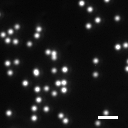
\includegraphics[width=\textwidth]{r01}
	\caption{}\label{fig:beads-widefield}
\end{subfigure}
\raisebox{9.3em}{\noindent\Huge$\Leftrightarrow$}
\begin{subfigure}[b]{0.45\textwidth}
	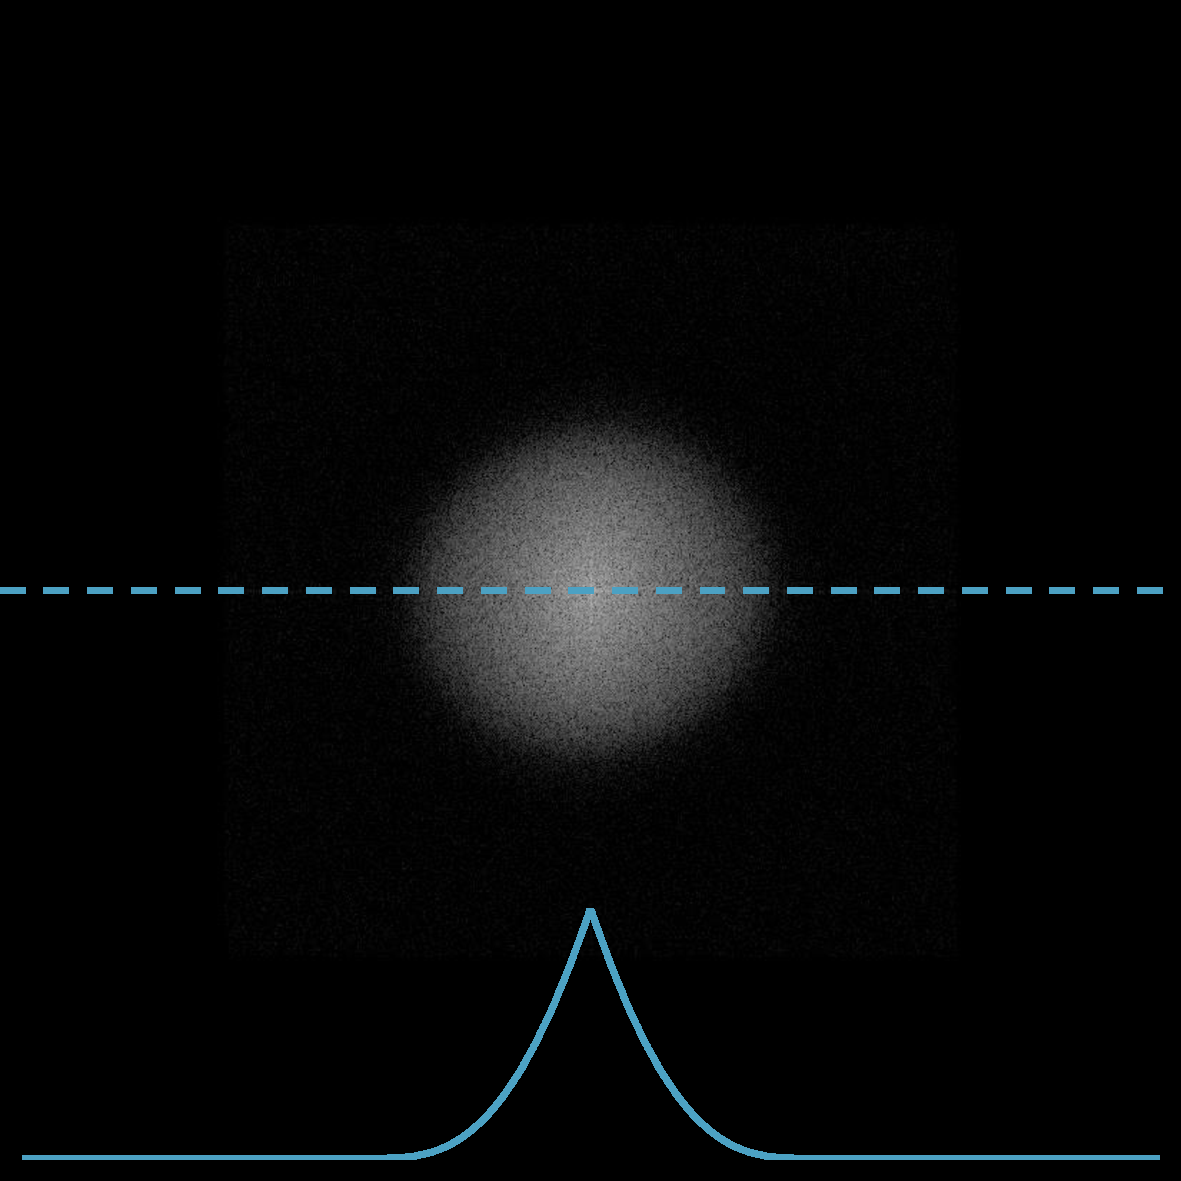
\includegraphics[width=\textwidth]{f01}
	\caption{}\label{fig:fourier-widefield}
\end{subfigure}
~\newline
\begin{subfigure}[b]{0.45\textwidth}
	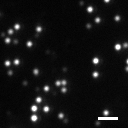
\includegraphics[width=\textwidth]{r02}
	\caption{}\label{fig:beads-raw-SIM}
\end{subfigure}
\raisebox{9.3em}{\noindent\Huge$\Leftrightarrow$}
\begin{subfigure}[b]{0.45\textwidth}
	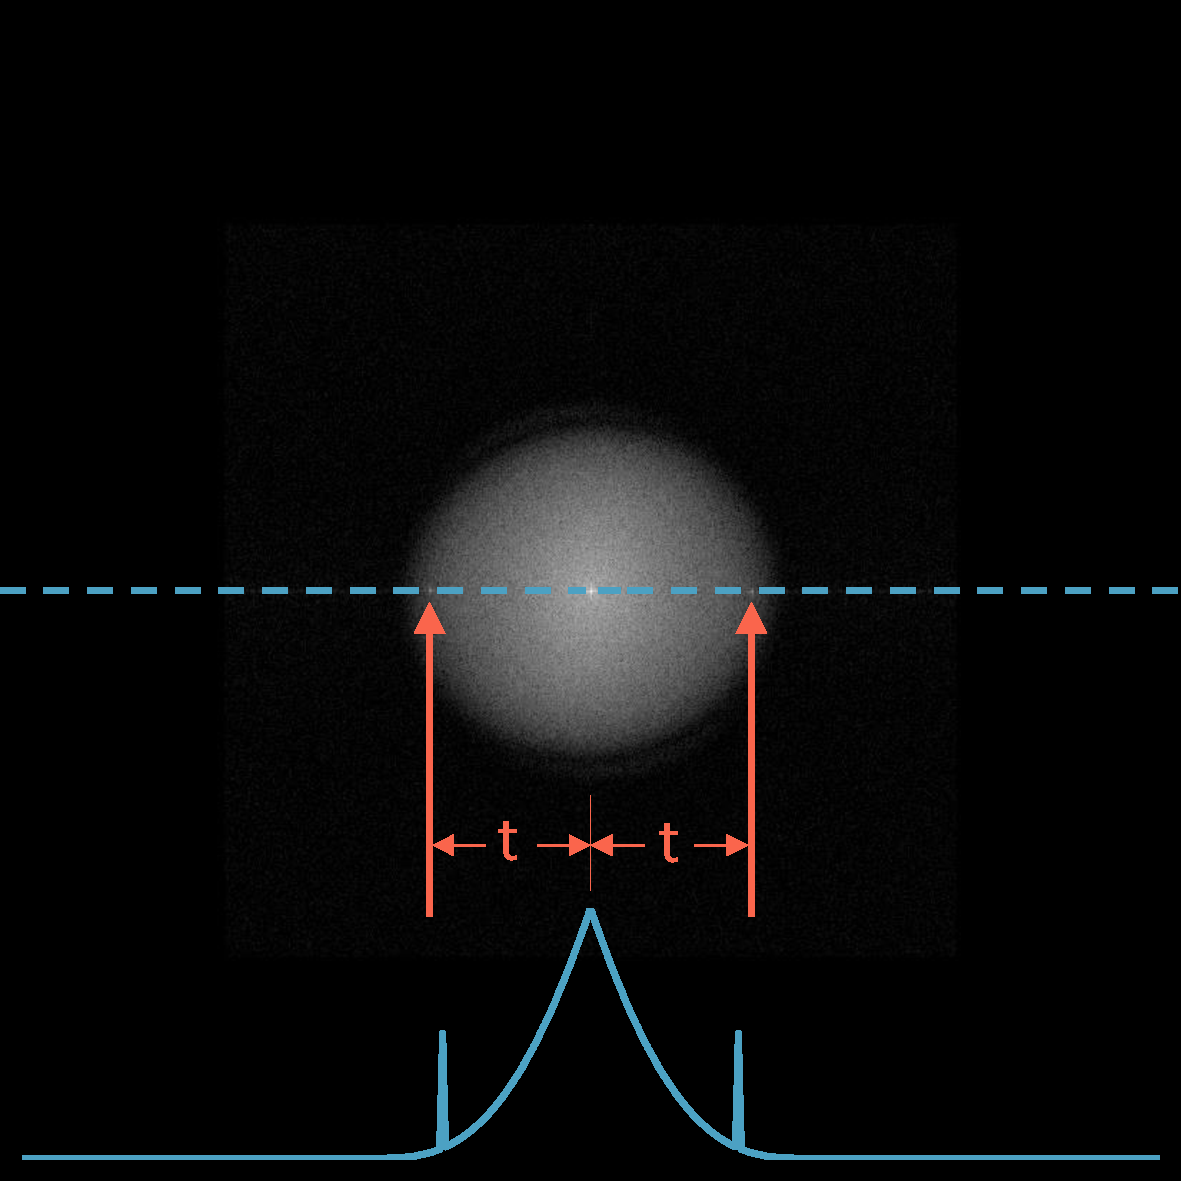
\includegraphics[width=\textwidth]{f02}
	\caption{}\label{fig:fourier-raw-SIM}
\end{subfigure}
~\newline
\begin{subfigure}[b]{0.45\textwidth}
	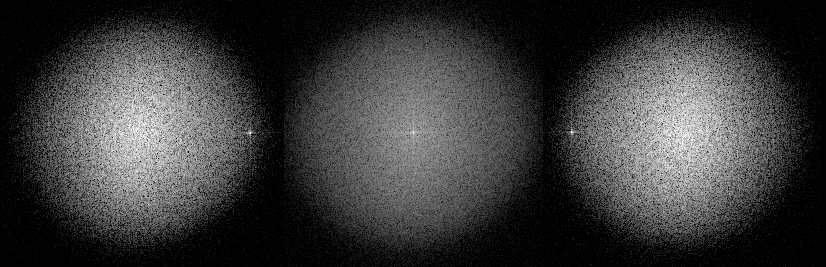
\includegraphics[width=\textwidth]{fourier-components}
	\caption{}\label{fig:fourier-components}
\end{subfigure}
\caption[LAG SIM: A sinusoidal illumination pattern is visible as delta peaks in Fourier space]{(a) shows a diffraction-limited image of \SI{100}{\nano\metre} beads.
(b) shows that spatial frequencies above the diffraction limit of the lens are not transmitted, causing a point-spread function which increases the apparent size of the beads and preventing two beads which are close together from being resolved.
(c) shows the same field of view under structured illumination; note that some beads are less intense than in (a) if they fall within a trough of the sinusoidal illumination pattern.
(d) clearly shows delta peaks appearing in the Fourier transform of (c) due to the sinusoidal illumination, at a distance from the origin equal to the spatial frequency of the illumination pattern.
(e) shows the Fourier components $\hat{H}\hat{S}\left(k_x\right)$, $\hat{H}\hat{S}\left(k_x+t\right)$, and $\hat{H}\hat{S}\left(k_x-t\right)$ extracted from the raw images by Equation~\ref{eq:matrix-inversion}. Scalebars are \SI{1}{\micro\metre}.
}
\label{fig:fourier-reconstruction}
\end{figure}

\begin{figure}[p]
\centering
\begin{subfigure}[b]{0.45\textwidth}
	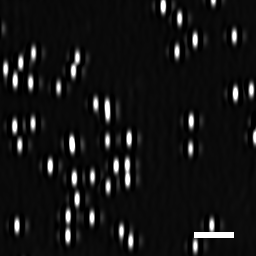
\includegraphics[width=\textwidth]{r04}
	\caption{}\label{fig:beads-x-doubling}
\end{subfigure}
\raisebox{9.3em}{\noindent\Huge$\Leftrightarrow$}
\begin{subfigure}[b]{0.45\textwidth}
	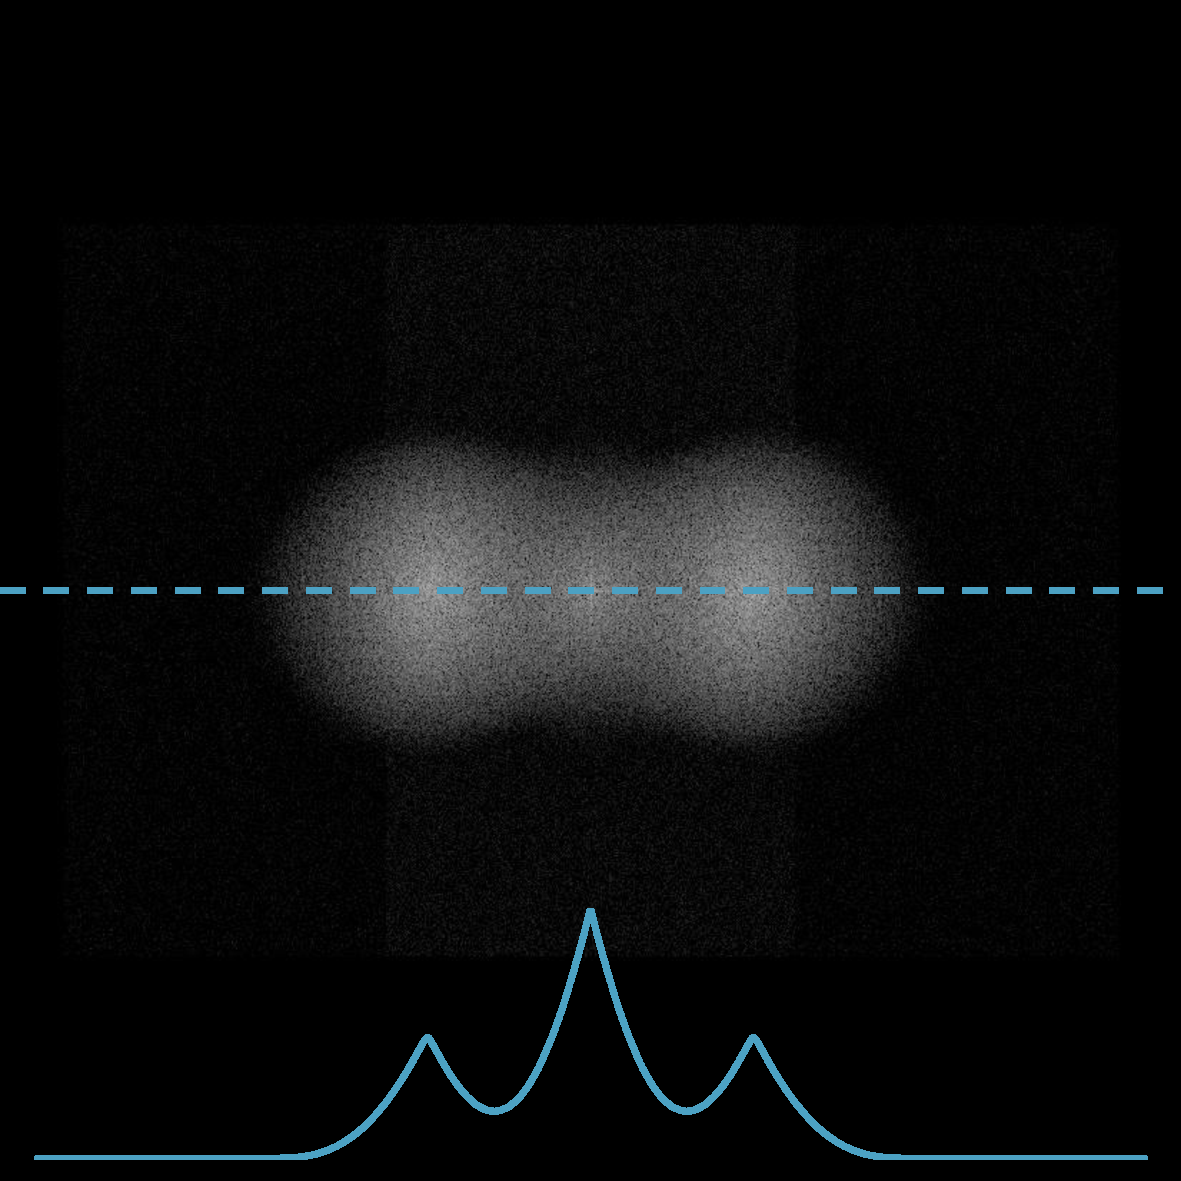
\includegraphics[width=\textwidth]{f04}
	\caption{}\label{fig:fourier-x-doubling}
\end{subfigure}
~\newline
\begin{subfigure}[b]{0.45\textwidth}
	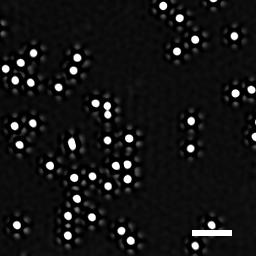
\includegraphics[width=\textwidth]{r05}
	\caption{}\label{fig:beads-isotropic-doubling}
\end{subfigure}
\raisebox{9.3em}{\noindent\Huge$\Leftrightarrow$}
\begin{subfigure}[b]{0.45\textwidth}
	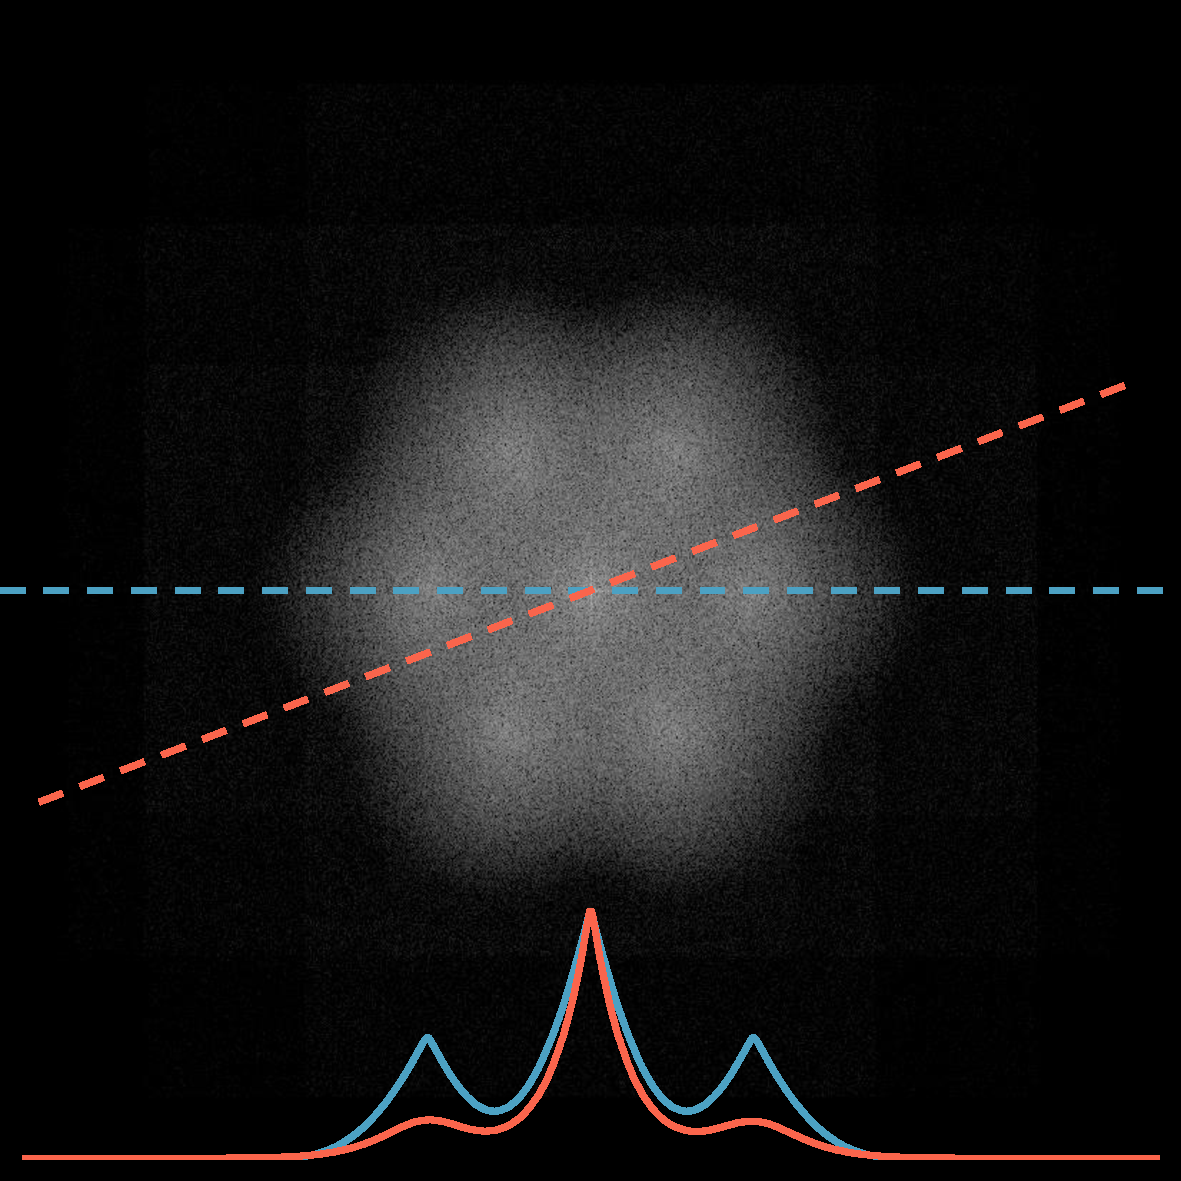
\includegraphics[width=\textwidth]{f05}
	\caption{}\label{fig:fourier-isotropic-doubling}
\end{subfigure}
\caption[LAG SIM: Reconstruction of SIM images takes place in Fourier space]{(a) shows beads after SIM reconstruction in the $x$-direction only, where the increase in $x$-resolution makes the circular beads appear as elongated ellipses.  (b) shows the corresponding Fourier-space image, where the width of the support confirms that resolution has doubled in the $x$-direction compared to widefield. (c) shows an isotropic increase in resolution, achieved by performing the procedure used to generate (a) at two more angles, \SI{60}{\degree} and \SI{120}{\degree} to the $x$-axis. (d) shows the Fourier transform of (c), confirming isotropic resolution increase. Notably, this reconstruction scheme produces peaks of signal in Fourier space and the OTF is not rotationally symmetric, causing the characteristic hexagonal artefacts visible in (c). Scalebars are \SI{1}{\micro\metre}.}
\label{fig:fourier-reconstruction}
\end{figure}

The same structured illumination microscopy (SIM) used for optical sectioning can be re-purposed for surpassing the diffraction limit.
First discussed by Lucosz~\cite{lukosz1966optical}, and then more explicitly described by Heintzmann for sinusoidal illumination patterns~\cite{heintzmann1999laterally}, the first experimental result showing 2D isotropic resolution doubling with 9 raw image acquisitions was published by Gustafsson in the year \num{2000}~\cite{gustafsson2000surpassing}.
Heintzmann shows that if we take the Fourier transform of the acquired images shown in Equation~\ref{eq:wilson-illumination}, we obtain the set of images shown in Equation~\ref{eq:heintzmann-fourier}; where \^{}-symbols represent 2D Fourier transforms of their equivalent variables, and $k_x$ is the Fourier variable of $x$, that is $f(x) \Leftrightarrow \hat{f}(k_x)$.
Note that $W$ has been replaced with its underlying components $H\otimes S \Leftrightarrow \hat{H}\hat{S}$, where $\hat{H}$, the Fourier transform of the PSF, is known as the optical transfer function (OTF).

\begin{equation} \label{eq:heintzmann-fourier}
\hat{I_i} = \hat{H} \hat{S} \otimes \left( \delta \left( k_x \right) + \frac{m}{2} e^{j\phi_i} \delta \left( k_x + t \right) + \frac{m}{2} e^{-j\phi_i} \delta \left( k_x - t \right) \right)
\end{equation}

Each acquired raw image contains contributions from each of 3 shifted Fourier components.
Using $\phi_i = \left\lbrace0, \frac{2\pi}{3}, \frac{4\pi}{3}\right\rbrace$, these Fourier components can be separated into individual images by solving the set of simultaneous equations for $\hat{S}\otimes\delta \left( k_x \right)$, $\hat{S}\otimes\delta \left( k_x + t \right)$, and $\hat{S}\otimes\delta \left( k_x - t \right)$ with matrix inversion, as shown in Figure~\ref{fig:fourier-components} and Equation~\ref{eq:matrix-inversion}~\cite{wicker2013phase}.
Assuming phase steps are all equal, performing a 3D Fourier transform of the phase-stepped raw images stacked in the 3rd dimension produces the same result~\cite{gustafsson2005nonlinear}.

\begin{equation} \label{eq:matrix-inversion}
\begin{bmatrix} \hat{H}\hat{S}\left(k_x\right) \\ \hat{H}\hat{S}\left(k_x+t\right) \\ \hat{H}\hat{S}\left(k_x-t\right) \end{bmatrix} =
\begin{bmatrix}
1 & \frac{m}{2}\exp\left(0j\right) & \frac{m}{2}\exp\left(-0j\right) \\
1 & \frac{m}{2}\exp\left(\frac{2\pi j}{3}\right) & \frac{m}{2}\exp\left(-\frac{2\pi j}{3}\right) \\
1 & \frac{m}{2}\exp\left(\frac{4\pi j}{3}\right) & \frac{m}{2}\exp\left(-\frac{4\pi j}{3}\right)
\end{bmatrix}^{-1}
\begin{bmatrix} \hat{I_1} \\ \hat{I_2} \\ \hat{I_3} \end{bmatrix}
\end{equation}

When the matrix of Equation~\ref{eq:matrix-inversion} is inverted, an factor of $m$ can be extracted as a scaling factor in front of the high frequency Fourier components, shown in Equation~\ref{eq:matrix-solved}.
In the same way that a smaller modulation depth $m$ reduces the signal-to-noise ratio in optical sectioning SIM, described in Section~\ref{sec:sim-background}, this factor shows that the signal-to-noise ratio of the high frequency components is directly proportional to the modulation depth of the illumination pattern.

\begin{equation} \label{eq:matrix-solved}
\begin{bmatrix} \hat{H}\hat{S}\left(k_x\right) \\ m\hat{H}\hat{S}\left(k_x+t\right) \\ m\hat{H}\hat{S}\left(k_x-t\right) \end{bmatrix} =
\frac{1}{3} \begin{bmatrix}
1 & 1 & 1 \\
2 & \left(-1 -\sqrt{3}j\right) & \left(-1+\sqrt{3}j\right) \\
2 & \left(-1 +\sqrt{3}j\right) & \left(-1 -\sqrt{3}j\right)
\end{bmatrix}
\begin{bmatrix} \hat{I_1} \\ \hat{I_2} \\ \hat{I_3} \end{bmatrix}
\end{equation}

To complete the reconstruction, the separated Fourier components must be placed at the correct position in Fourier space, as determined by $t$.
Assuming the sinusoidal illumination pattern is generated by the same lens used for imaging the sample, the highest frequency sinusoid which can be generated will correspond to delta peaks at the edge of the microscope's support in Fourier space~\cite{heintzmann2017super}, visible in Figure~\ref{fig:fourier-raw-SIM}.
When the components are shifted into the appropriate location, the support of the OTF doubles in the $x$-direction, as shown in Figure~\ref{fig:fourier-x-doubling}.
Figure~\ref{fig:beads-x-doubling} confirms that resolution is doubled in the $x$-direction, which makes the circular beads appear as elongated ellipses.

To achieve isotropic 2D resolution doubling, the sinusoidal illumination pattern must be rotated to cover more area in Fourier space.
Typically a total of three rotations are used, at \SI{60}{\degree} and \SI{120}{\degree} to the original pattern orientation~\cite{gustafsson2000surpassing, chang2009isotropic}.
Performing the reconstruction procedure on all 9 images produces the Fourier space reconstruction shown in Figure~\ref{fig:fourier-isotropic-doubling}, showing an isotropic increase in the resolution support.
% Support is the closure of the set of points at which the Fourier transform takes a non-zero value


The final step for this reconstruction procedure is to inverse Fourier transform the reconstructed Fourier space image of Figure~\ref{fig:fourier-isotropic-doubling} to produce Figure~\ref{fig:beads-isotropic-doubling}, an image with double the equivalent widefield resolution.
Comparing Figure~\ref{fig:beads-isotropic-doubling} to Figure~\ref{fig:beads-widefield}, the beads appear smaller and two close beads which could not be resolved before can now be distinguished.
However, the reconstruction procedure must be refined to reduce the hexagonal artefacts introduced by this reconstruction method.

\subsection{Refining the reconstruction algorithm reduces artefacts}
The 2D OTF of a focussed lens is a rotationally symmetric function which gradually reduces to zero as spatial frequency increases~\cite{williams2002introduction}.
The line profile through the OTF of an ideal lens in Figure~\ref{fig:fourier-widefield} shows that the higher the spatial frequency, the less contrast the microscope produces.
In a practical set-up, noise further limits the resolvable contrast at high frequencies, such that signal-to-noise ratio decreases as spatial frequency increases.

\begin{figure}[tbp]
\vspace{-6pt} \centering
\begin{subfigure}[b]{0.45\textwidth}
	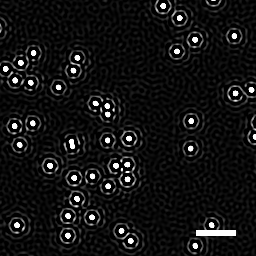
\includegraphics[width=\textwidth]{r06}
	\caption{}\label{fig:beads-wiener}
\end{subfigure}
\raisebox{9.3em}{\noindent\Huge$\Leftrightarrow$}
\begin{subfigure}[b]{0.45\textwidth}
	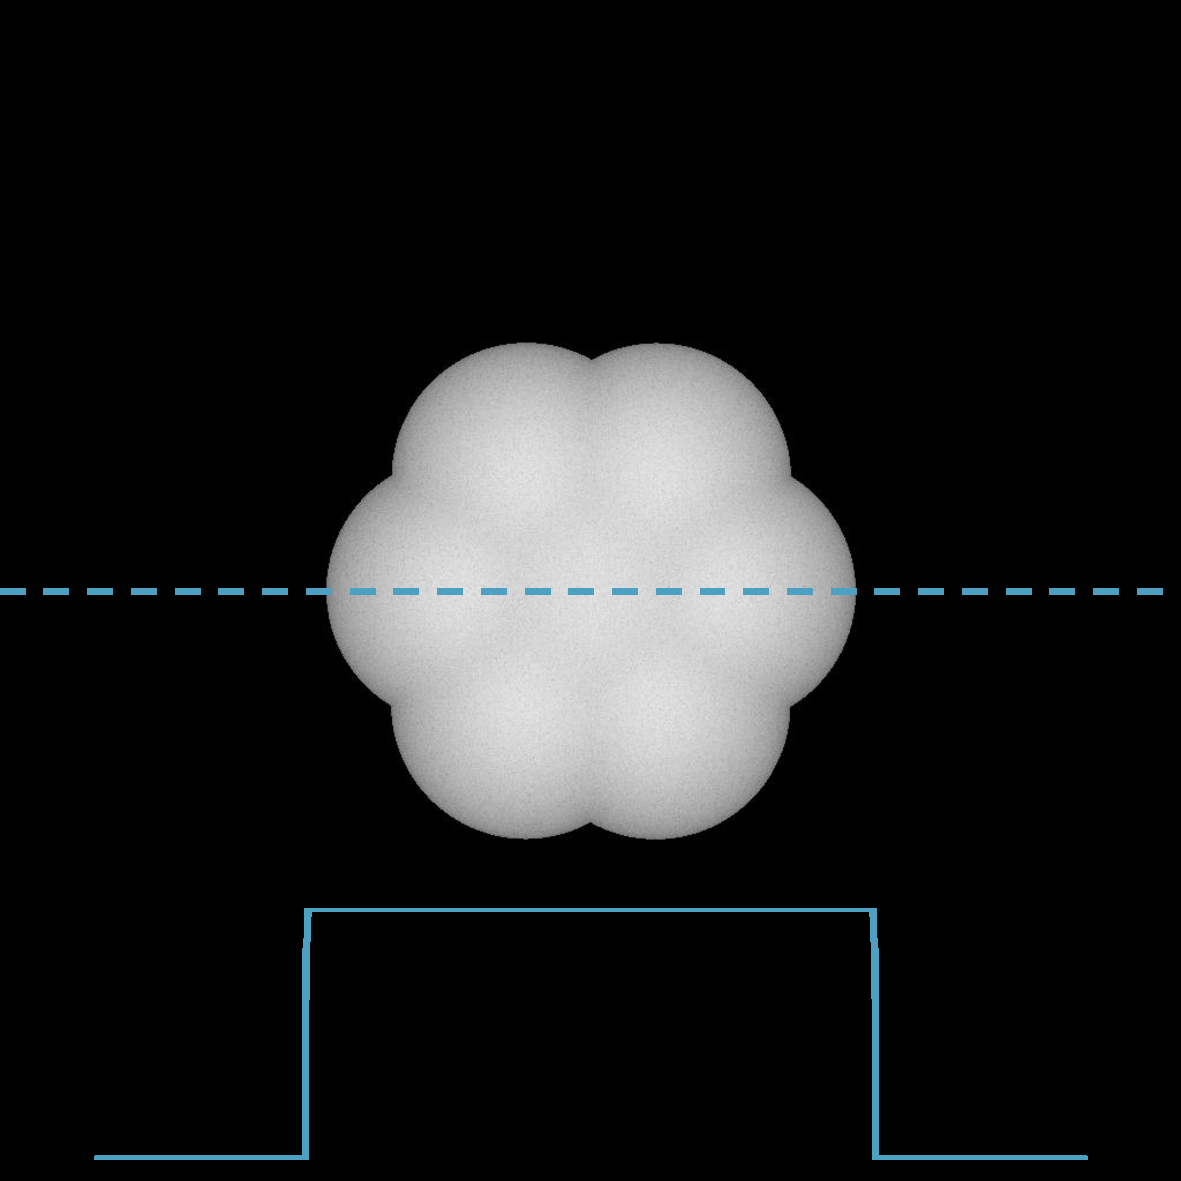
\includegraphics[width=\textwidth]{f06}
	\caption{}\label{fig:fourier-wiener}
\end{subfigure}

~\newline
\begin{subfigure}[b]{0.45\textwidth}
	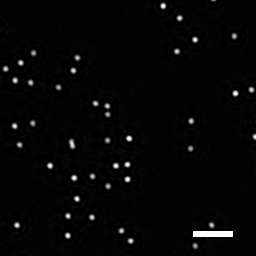
\includegraphics[width=\textwidth]{r07}
	\caption{}\label{fig:beads-apodised}
\end{subfigure}
\raisebox{9.3em}{\noindent\Huge$\Leftrightarrow$}
\begin{subfigure}[b]{0.45\textwidth}
	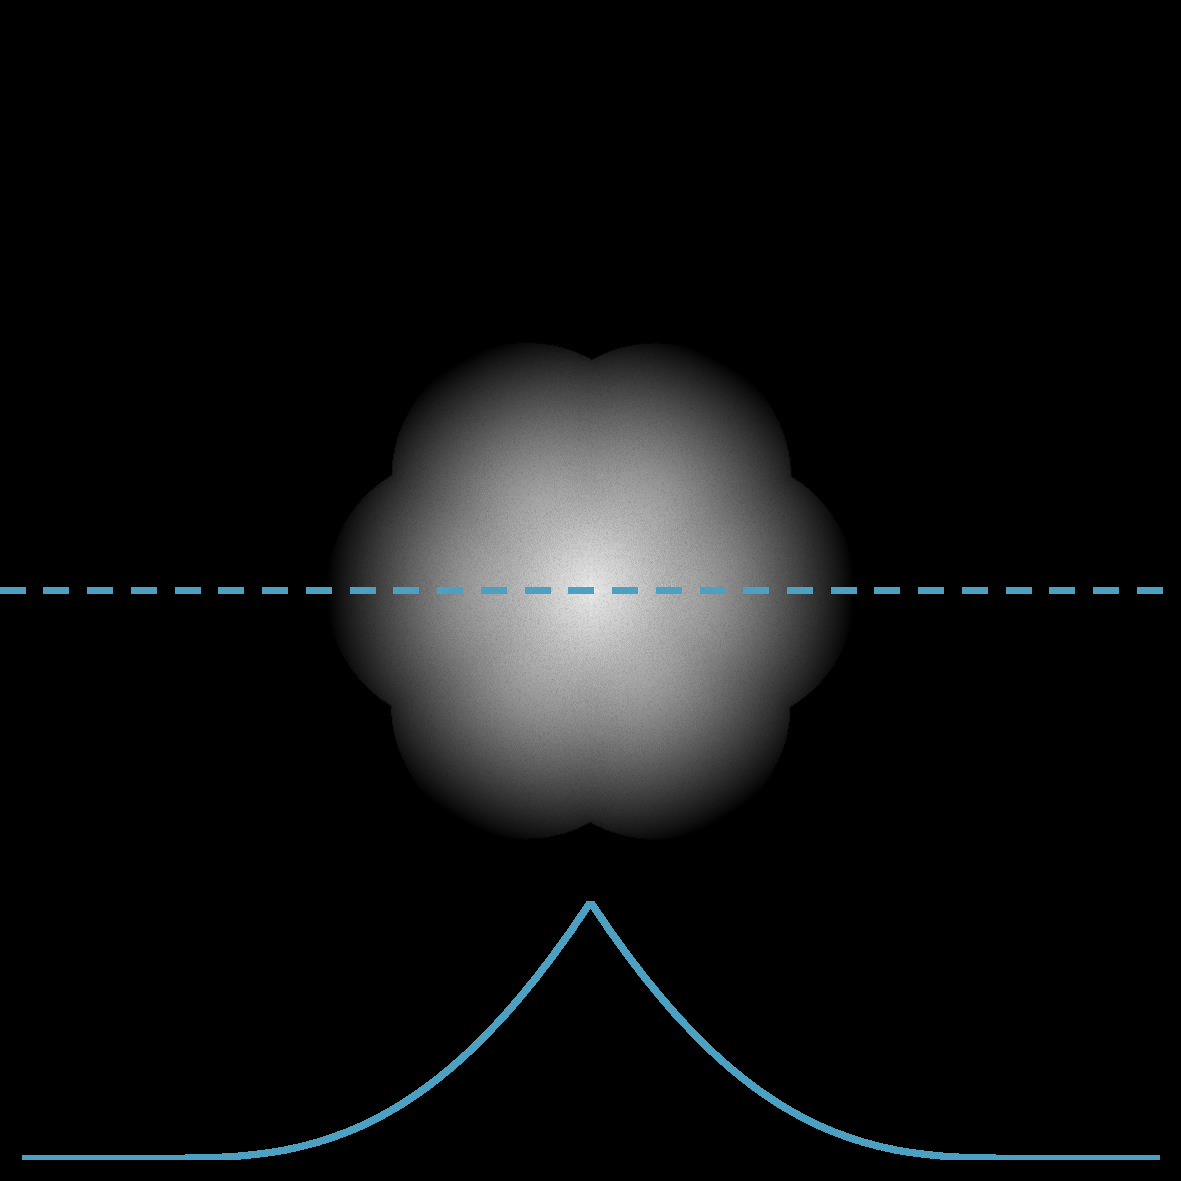
\includegraphics[width=\textwidth]{f07}
	\caption{}\label{fig:fourier-apodised}
\end{subfigure}
\caption[LAG SIM: Wiener filtering of the SIM OTF is required for artefact-free reconstruction]{(a) shows a reconstructed SIM image after Wiener filtering described in Equation~\ref{eq:wiener-filtering}, with $A\left(k\right) = 1$.
(b) shows that this filtering produces a flat OTF in Fourier space, which is also rotationally symmetric.
However, the sharp cutoff of the Fourier space support causes ringing in the reconstructed image, clearly visible around the beads in (a); although compared to Figure~\ref{fig:beads-isotropic-doubling} the artefacts are now rotationally symmetric, rather than honeycombed.
To reduce ringing artefacts, and produce the high-resolution bead image shown in (c), an apodisation filter which gradually decreases is applied to (b), as shown in (d).
Comparing (d) to Figure~\ref{fig:fourier-widefield} shows an isotropic doubling in the OTF's support; consequently, comparing the beads in (c) to Figure~\ref{fig:beads-widefield} shows a smaller point spread function, allowing two beads to be distinguished which were previously too close to resolve. Scalebars are \SI{1}{\micro\metre}.}
\label{fig:sim-OTFs}
\end{figure}

The signal-to-noise ratio's relationship with spatial frequency has a particularly dramatic effect in SIM.
Equation~\ref{eq:matrix-inversion} shows that each shifted frequency component, $\hat{S}_i$, is apodised by the microscope OTF, $\hat{H}$.
It can be clearly seen in Figure~\ref{fig:fourier-x-doubling} that this results in an overall OTF which does not gradually decrease, but rather has peaks at certain frequencies.
These peaks translate directly to frequency peaks in the signal-to-noise ratio, therefore the noise pattern in the reconstructed image is no longer white noise with equal power at all frequencies.
Furthermore, it can be seen in Figure~\ref{fig:fourier-isotropic-doubling} that the reconstructed SIM OTF is not rotationally symmetric.
These two aspects combine to cause characteristic hexagonal honeycomb artefacts in reconstructed SIM images~\cite{wicker2013phase}, clearly visible in Figure~\ref{fig:beads-isotropic-doubling}.

To reduce these artefacts, Fourier components are reconstructed through a de-noising algorithm.
The most common practice is to combine the frequency components through a generalised Wiener filter~\cite{gustafsson2008three}, as shown in Equation~\ref{eq:wiener-filtering}, to produce the reconstructed image $\hat{I_R}$.
Note that this equation now describes the general 2D or 3D case, where $\mathbf{k}$ is a vector of Fourier variables and $\mathbf{p}$ is a vector in the direction of the sinusoidal illumination pattern for each direction $d$.
$w^2$ is a constant, adjusted empirically depending on the level of noise in the image, and $A\left(\mathbf{k}\right)$ is an apodisation function.

\begin{equation} \label{eq:wiener-filtering}
\hat{I_R} = \frac{\sum_{d,i}\hat{H}^*\left(\mathbf{k} + \phi_i\mathbf{p}_d\right) \hat{S}_{d,i}\left(\mathbf{k} + \phi_i\mathbf{p}_d\right)} {\sum_{d,i}\abs{\hat{H}\left(\mathbf{k} + \phi_i\mathbf{p}_d\right)}^2 + w^2} A\left(\mathbf{k}\right)
\end{equation}

If $A\left(\mathbf{k}\right)=1$, this reconstruction scheme removes the decaying characteristic of the OTF, instead making a flat top-hat function shown in Figure~\ref{fig:fourier-wiener} which suddenly cuts off at the doubled resolution limit.
However, because the Fourier transform of a top-hat function is a sinc function, this causes ringing artefacts in the reconstructed image~\cite[\textit{ch. 10}]{kreyszig2006advanced}.
Ringing is clearly visible in Figure~\ref{fig:beads-wiener}, although compared to Figure~\ref{fig:beads-isotropic-doubling} the artefact is now rotationally symmetric rather than honeycombed.
To remove rinigng, the apodisation function $A\left(\mathbf{k}\right)$ is chosen as a filter which decays from the 0 frequency to the new resolution limit, for example a Gaussian filter shown in Figure~\ref{fig:fourier-apodised}~\cite{nixon2016increased}.

More recent research suggests improvements to generalised Wiener filtering~\cite{righolt2013image, perez2016optimal, chakrova2016deconvolution}, and a detailed discussion of alternative filtering schemes follows in Section~\ref{sec:recon} of this chapter.


\subsection{Aims for LAG SIM}
When I arrived in the Laser Analytics Group (LAG) a SIM microscope designed by Laurie Young was reaching the end of its practical life~\cite{young2016guide}.
Issues with device degradation, detailed in Section~\ref{sec:lagsim-pockels}, limited the imaging speed to \SI{0.1}{\hertz}.
Furthermore, a complicated ensemble of software required an expert user to operate the microscope.

A physical relocation of the laboratory in early 2017~\cite{newbuilding} provided the ideal opportunity to rebuild the microscope and the associated control software. The first priority was to restore the microscope to \SI{11}{\hertz} imaging speed. Once this was achieved, a list of several other aims were devised:
\begin{enumerate}
	\item Provide an easy method to switch between optical sectioning SIM and resolution-doubling SIM in TIRF (Sections~\ref{sec:hardware} and \ref{sec:labview}).
	\item Split the fluorescence emission light at the output of the microscope to facilitate simultaneous capture of multiple colour channels (Section~\ref{sec:lagsim-path}).
	\item Re-write the control software to make the microscope user-friendly for a non-expert user to operate unsupervised (Section~\ref{sec:labview}).
	\item Design reconstruction software to allow users to quickly reconstruct artefact-free images without detailed knowledge of reconstruction algorithms (Sections~\ref{sec:recon} and \ref{sec:lagsimFiji}).
\end{enumerate}

As well as detailing solutions to these challenges, this chapter also presents a showcase of various biological experiments performed with LAG SIM.
Section~\ref{sec:sim-showcase} can therefore be used a collection of case-study examples for anyone wishing to run similar investigations.

\section{SIM hardware} \label{sec:hardware}
\subsection{Optical path design to generate a SIM pattern} \label{sec:lagsim-path}
As part of his PhD work from 2012-2016, Dr. Laurie Young designed and built a SIM microscope in the Laser Analytics Group~\cite{young2016guide}.
The rebuilt SIM setup, `LAG SIM,' is based heavily on this original design, but with several modifications which were implemented by me when the Group moved location in February 2017.

\begin{sidewaysfigure}[p]
\centering
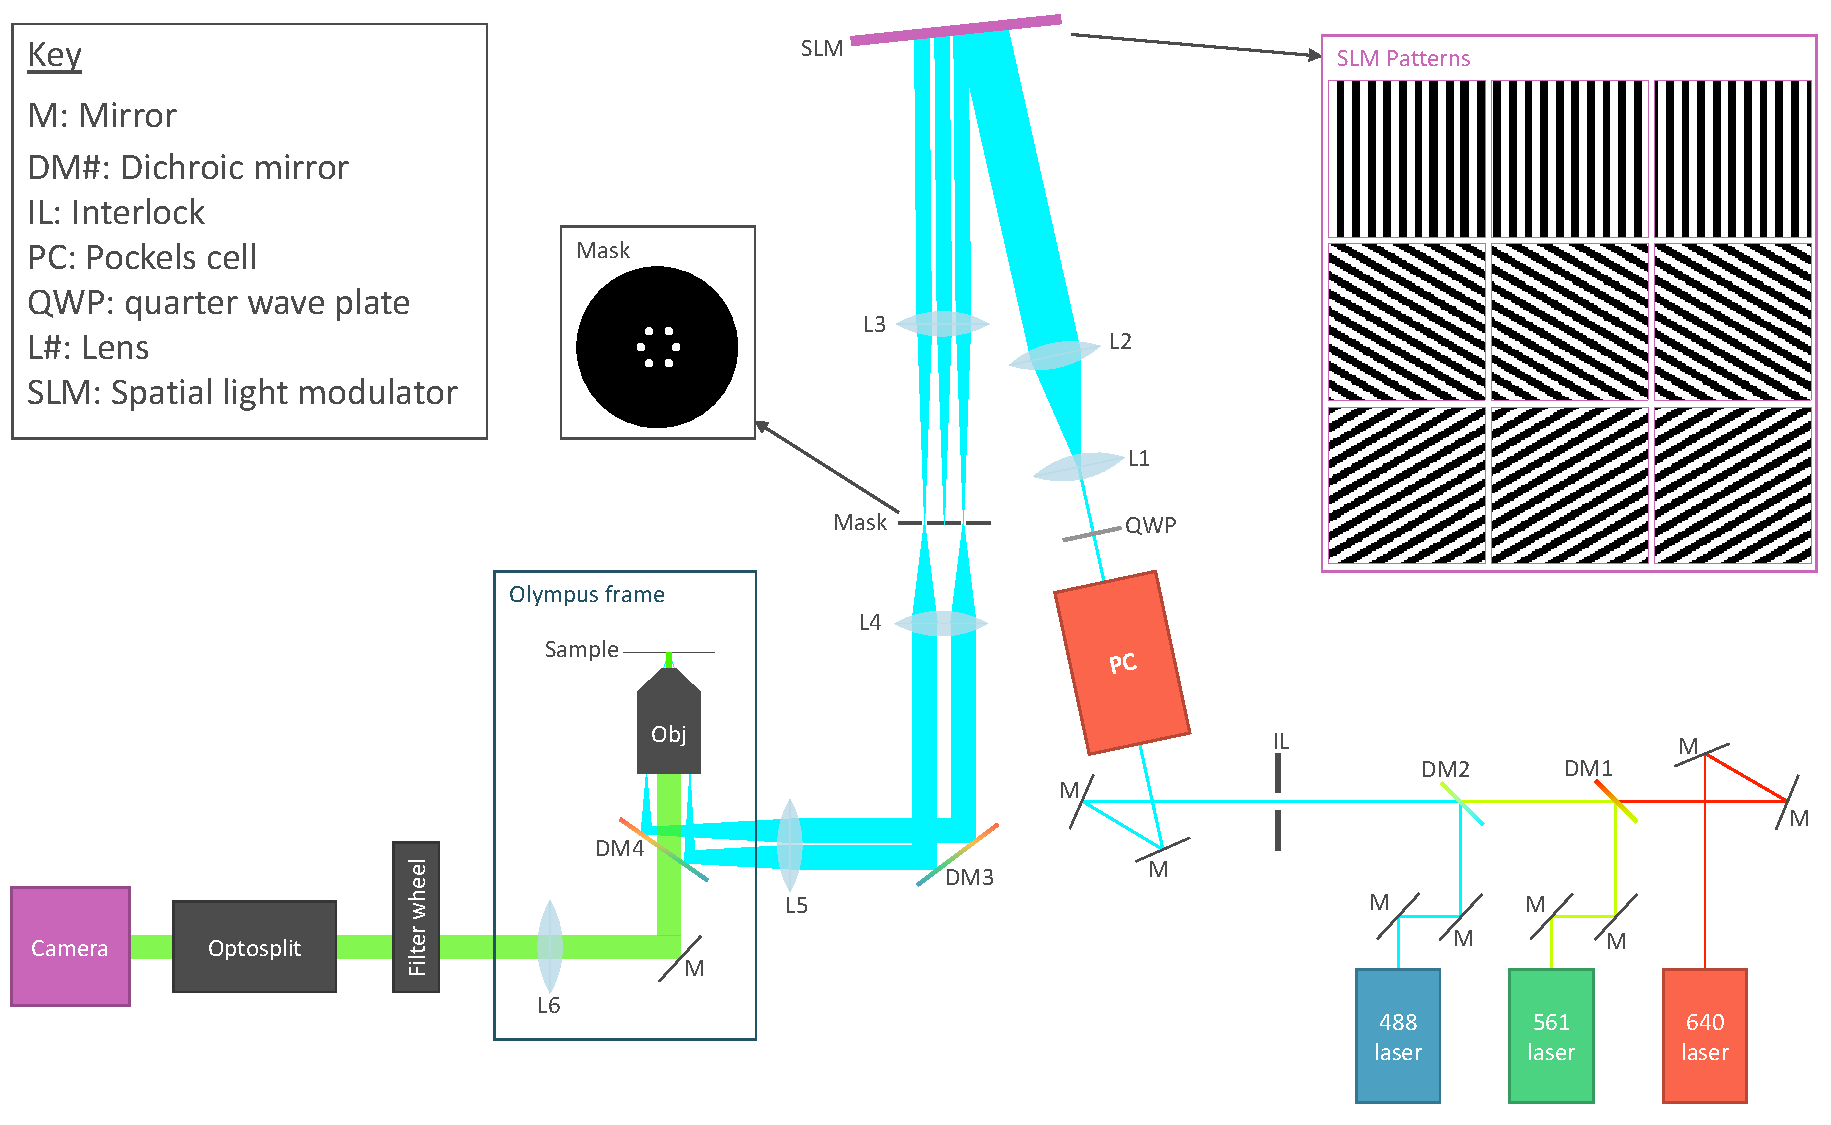
\includegraphics[width=0.92\textwidth]{sim-optical-path}
\caption[LAG SIM: Various optics work together to pattern the laser light with a SIM pattern and apply polarisation rotation for optical sectioning and resolution enhancement]{The optical layout of the SIM aligns light from one of 3 lasers onto an optical path. The light passes through a Pockels cell and quarter wave plate for polarisation rotation, before a square-wave pattern is applied by a spatial light modulator. The patterned light is passed through a spatial mask in the Fourier plane to produce a sinusoidal pattern, which is relayed onto the sample. The objective lens collects fluorescent emission light,  which is filtered to remove any reflected excitation light before reaching the sCMOS camera.}
\label{fig:SIMpath}
\end{sidewaysfigure}

The optical path diagram is shown in Figure~\ref{fig:SIMpath}, and works as follows: laser light is generated by one of three lasers at a wavelength of \SI{488}{\nano\metre}, \SI{561}{\nano\metre}, or \SI{640}{\nano\metre}; its polarisation is aligned with the direction of the structured illumination pattern by a Pockels cell and achromatic quarter-wave plate; it passes through a beam expander so that it fully covers the spatial light modulator (SLM) display; it reflects and diffracts off the SLM display, which is displaying a binary diffraction grating; it passes through a `beam minimiser' (a beam expander in reverse) so that it is an appropriate size for the microscope lenses; it passes through a spatial filter at a Fourier plane, which removes all but the ±1 diffraction orders from the SLM diffraction; it reflects off of a dichroic mirror; it passes into the microscope's tube lens; it reflects off of a second dichoric mirror; and finally it passes into the objective lens and is focussed onto the sample.
DM3 and DM4 are sourced from the same manufacturing batch, so that any aberrations introduced by non-uniformity of DM3 are undone upon reflection from DM4.

This effectively images a low-pass-filtered version of the SLM's diffraction grating onto the sample.
The spatial filter means that the binary grating becomes a sinusoidal pattern, with the distance between peaks set by (a) the period of the diffraction grating shown on the SLM display and (b) the demagnification of the system from SLM to sample.
An equivalent way of conceptualising this is to picture the two filtered beams of light entering the rear focal plane of the objective lens, such that they produce an interference pattern when they meet at the sample plane~\cite[\textit{ch. 9}]{hecht2017optics}.
The result is a sinusoidal illumination pattern at the sample plane, the orientation and period of which can be set by binary patterns shown on the SLM.

This SIM is a fluorescence microscope, so that, assuming linear fluorophore behaviour~\cite{gustafsson2005nonlinear, shen1984principles}, the amount of light emitted from a point in the sample is proportional to the amount of light illuminating that point, but the emission light is at a different wavelength to the illumination light.
In the LAG SIM microscope, fluorescent emission light travels back through the objective lens, through the dichroic mirror and towards the camera to record a 2D image.
Before it reaches the camera, it is filtered in one of two ways to remove any reflected illumination light.
The first option is to use a filter wheel, which contains three filters appropriate for removing the illumination light and can be switched via a serial command from the computer.
The second option is to use the Optosplit III from Cairn Research, which uses filter cubes to split the emission light into three paths directed onto separate areas of the camera, facilitating simultaneous imaging of three colour channels.

The Optosplit provides a significant increase in speed for multicolour imaging.
In this setup, the fastest speed at which the camera can reliably record images without dropping frames is \SI{10}{\milli\second}.
A SIM reconstruction requires 9 images, giving a total exposure time of \SI{90}{\milli\second} per channel; however switching channels with the filter wheel adds an additional \SI{100}{\milli\second} as the wheel rotates to the next filter and settles.
For a 3-colour image using the filter wheel, the fastest SIM imaging rate is therefore \SI{570}{\milli\second} per frame, or \SI{1.75}{\hertz}.
Using the Optosplit is over 6 times faster, providing a maximum \SI{11.1}{\hertz} imaging rate even for multicolour images.

Finally, an autofocus system between the microscope frame and filter wheel works with the z-control of the microscope stage to maintain a constant focus on the sample.
This is useful in two scenarios.
Firstly, when a timelapse sequence is captured over a number of hours, the microscope lens drifts downwards away from the sample.
Without the autofocus system, this would result in a loss of focus; however by automatically moving the stage as the lens drifts, focus can be maintained over a period of days.
Secondly, if a large field of view is captured to create a mosaic of images, focus can be lost due to the cover glass not being perfectly flat.
Again, the autofocus system holds focus over this full field of view, allowing large areas to be imaged.


\subsection{A Pockels cell provides fast polarisation rotation} \label{sec:lagsim-pockels}
In the SIM excitation path, a Pockels cell is used to rotate the polarisation of the illumination light so that it is aligned with the sinusoidal SIM pattern.

In SIM, it is important that the modulation contrast is as large as possible, that is, that the troughs of the sinusoidal illumination pattern are as dark as possible.
When the 9 raw images are computationally recombined, the signal-to-noise ratio of high-spatial-frequency components is directly proportional to the modulation contrast~\cite{oholleran2012polarization}, as described in Section~\ref{sec:SIM-theory}.

Modulation contrast of fluorescence emission light can be degraded by a number of sources, including out-of-focus light and aberrations in the imaging system, which is unavoidable in thick samples.
Furthermore, if the polarisation of the illumination light is not rotated to align with the rotations of the SIM pattern,  modulation contrast is degraded due to the effects of a high numerical aperture lens.

Two waves with orthogonal polarisation will not interfere~\cite{nityananda2013interference}.
As light passes through a high numerical aperture lens, the polarisation state which is parallel to the meridional plane (p-polarised) is rotated; whereas the polarisation state perpendicular (s-polarised) is unaffected~\cite{mansuripur1991effects}.
To ensure that light from the two beams entering the back-aperture of the lens arrive at sample plane with the same polarisation, it is therefore necessary that the light is entirely s-polarised~\cite{oholleran2012polarization}.

If the meridional plane is defined at an angle of $\theta=0\si{\degree}$ around the optical axis, aligned with the back-aperture spots when the SLM is showing a vertical SIM grating pattern, the incident light should be linearly polarised at $\theta=90\si{\degree}$ to ensure s-polarised light, as shown in Figure~\ref{fig:meridional-plane}.
However, for 2D isotropic resolution enhancement, the SIM pattern must also be rotated to $\pm60\si{\degree}$.
For these patterns the $\theta=90\si{\degree}$ polarisation of the light does not represent s-polarised light.
In order to maintain s-polarised light, thereby ensuring maximum pattern contrast, the polarisation must be rotated to align with each orientation of the SIM pattern.

\begin{figure}[tbp]
\centering
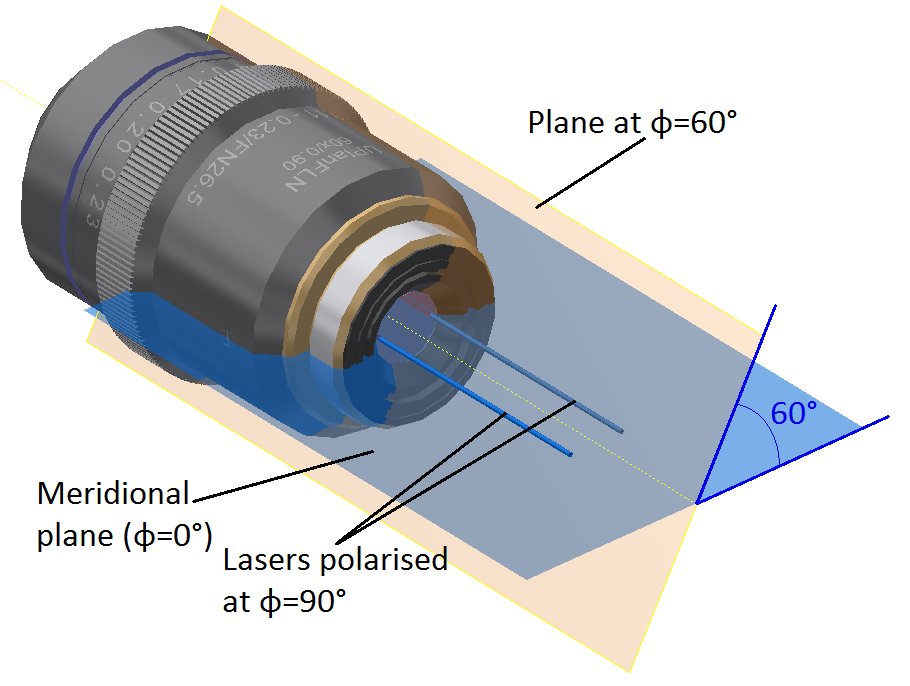
\includegraphics[width=\textwidth]{meridional-plane}
\caption[LAG SIM: Laser polarisation must be perpendicular to the sinusoidal illumination for high pattern contrast]{To ensure maximum pattern contrast, the excitation laser light must be s-polarised - that is, polarised at \SI{90}{\degree} to the meridional plane for the vertical sinusoidal illumination pattern. When the illumination pattern is rotated to $\pm60\si{\degree}$, $\theta=90\si{\degree}$ polarisation no longer produces s-polarised light. If the polarisation is not rotated to align with the rotated illumination pattern, some p-polarised light will enter the objective, which is rotated as it passes through the high NA lens. The p-polarised light will therefore not interfer at the sample plane, reducing the contrast of the illumination pattern.} \label{fig:meridional-plane}
\end{figure}

The original SIM system, detailed in reference~\cite{young2016guide}, used a liquid crystal variable retarder (LCVR) to rotate the polarisation to align with the SLM's grating orientation.
This suffered an unexpected problem where the laser beam damaged the liquid crystal material leaving a visible spot on the LCVR and no longer retarded the light, so the system no longer rotated polarisation.
The product line has since been discontinued.
As an interim solution, an achromatic half-wave plate was mounted in a serial-controlled rotation stage in place of the LCVR~\cite[\textit{ch. 8}]{hecht2017optics}.
This setup successfully rotated the polarisation and ensured good modulation contrast, but was only able to image at \SI{0.1}{\hertz}.

For fast and reliable polarisation rotation, facilitating \SI{11}{\hertz} SIM imaging, we purchased a Pockels cell from Conoptics.
Similarly to the LCVR, a Pockels cell provides voltage-controlled retardation of one polarisation axis which, in combination with a quarter-wave plate, creates rotation of linear polarisation~\cite[\textit{ch. 8}]{hecht2017optics}.
The level of retardation is controlled by a voltage across the Pockels cell, restoring polarisation rotation with no mechanical movement.

\subsection{Pockels cell alignment procedure} \label{sec:alignment-procedure}
To use the Pockels cell as a polarisation rotator, light entering the cell must be linearly polarised and aligned at \SI{45}{\degree} to the fast axis of the device.
The Pockels cell from Conoptics Inc. was delivered with a Glan-Taylor polariser appropriately aligned in the factory.

To align the Pockels cell to the rest of the system, the following procedure was devised, with the voltage across the Pockels cell set to \SI{0}{\volt}: % Shown in figure?
\begin{enumerate}
	\item Place the Pockels cell in 5-axis mount
	\item Coarsely align so that the beam passes through the centre of the Pockels cell
	\item Using a power meter after the Pockels cell, rotate the cell until power is maximised
	\item Adjust the tip-tilt of the Pockels cell, maximising power again
	\item Insert a linear polariser between the Pockels cell and power meter, and rotate the polariser until power is maximised
	\item Insert the quarter-wave plate (QWP) into the beam path mounted in a rotation mount between the Pockels cell and linear polariser
	\item With the power meter after the QWP, rotate the QWP until power is maximised, as shown in Figure~\ref{fig:alignment-photo}
	\item Remove the linear polariser
\end{enumerate}

Although this alignment procedure could be completed with any laser, for LAG SIM it is best to use the \SI{561}{\nano\metre} laser, as this is the closest to the centre wavelength of the achromatic quarter-wave plate.

\begin{figure}[htbp!]
\centering
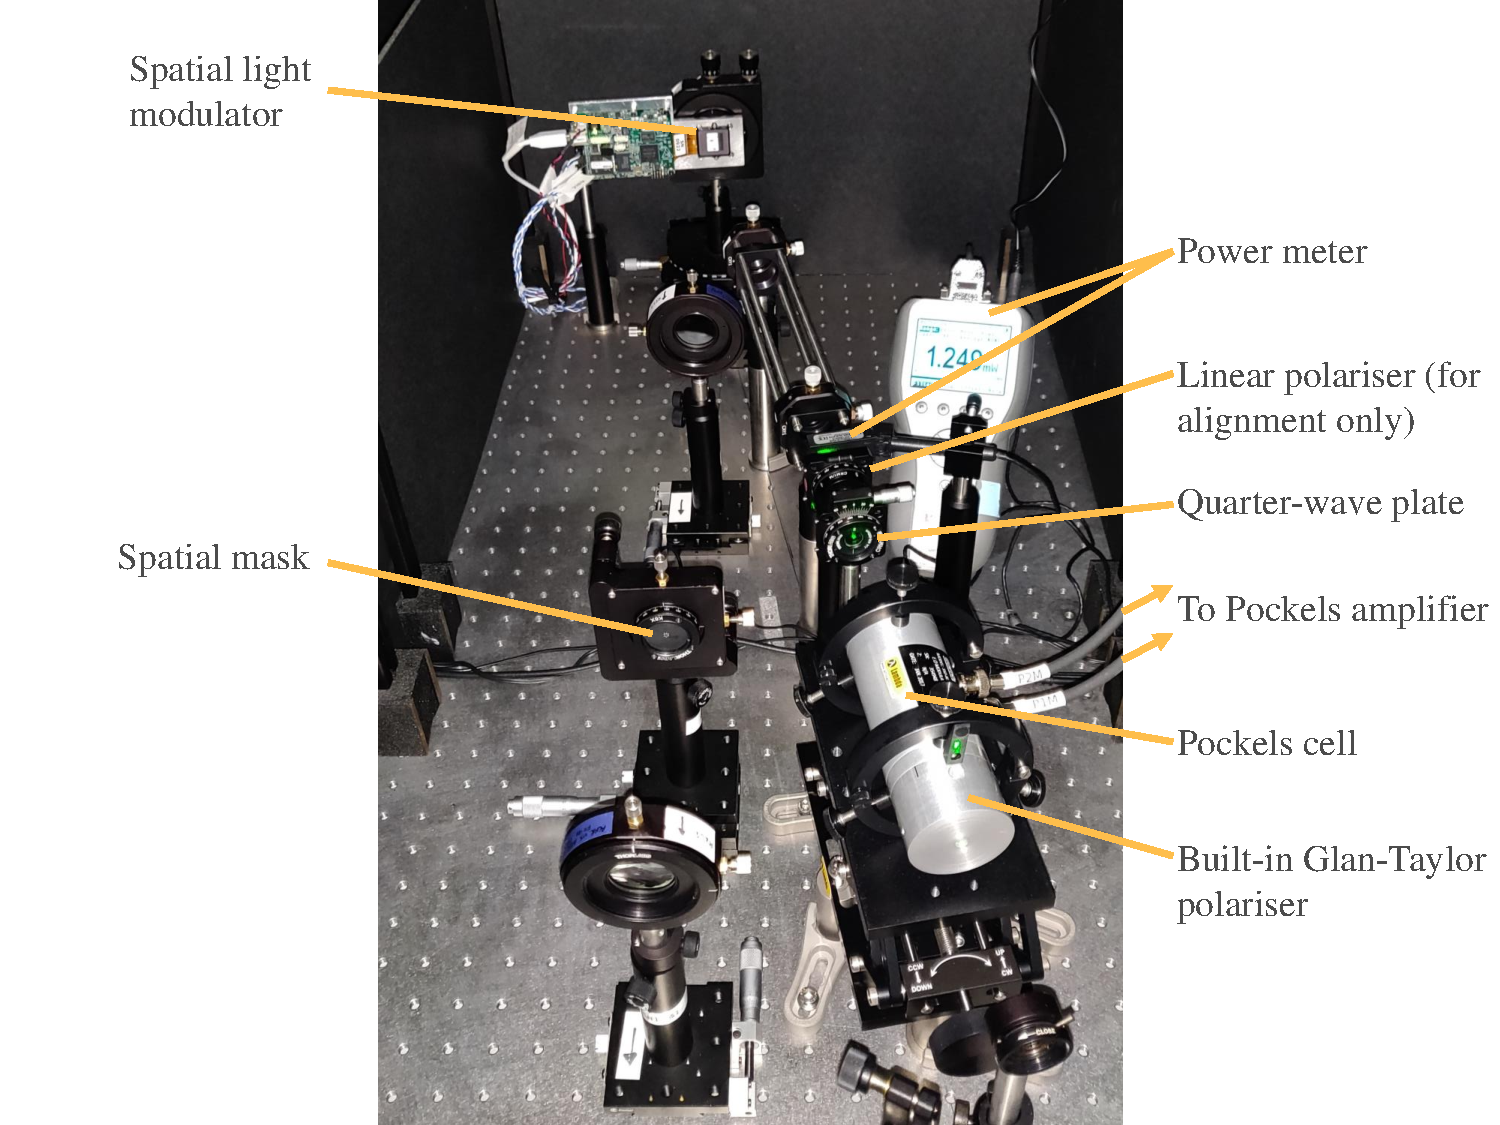
\includegraphics[width=1.0\textwidth]{alignment-photo}
\caption[LAG SIM: Alignment of the Pockels cell and quarter-wave plate to facilitate fast linear polarisation rotation]{The photo shows the LAG SIM beam path during alignment of the Pockels cell. A power meter is used in combination with a linear polariser to measure the polarisation rotation of the beam after retardation of one polarisation axis by the Pockels cell and quarter wave plate. Alignment is performed as per the protocol described in Section~\ref{sec:alignment-procedure}. Also visible are the spatial light modulator and spatial mask, which are used in combination to generate the sinusoidal illumination pattern.}
\label{fig:alignment-photo}
\end{figure}


The polarisation state of the light was measured to ensure the Pockels cell was behaving as expected by using a linear polariser in a rotation mount as an analyser before the power meter, as shown in Figure~\ref{fig:alignment-photo}.
The laser emission entering the Pockels cell was linearly polarised, with an extinction ratio of 100:1 for the \SI{561}{\nano\metre} laser.
The Glan-Taylor polariser theoretically increases the extinction ratio to >\num{100000}:1~\cite{bennett1995handbook}, although because it is attached to the Pockels cell in the factory, as seen in Figure~\ref{fig:alignment-photo}, this extinction ratio cannot be measured.
Light exiting the Pockels cell is elliptically polarised, with the degree of ellipticity determined by the voltage.
Finally, the QWP restores the elliptically polarised light to linear polarisation, but rotated compared to the input as determined by the voltage over the Pockels cell.
The extinction ratio at the output of the QWP was 500:1.

\subsection{Measuring Pockels cell voltages for optimal pattern contrast}
The voltage across the Pockels cell determines the amount of optical anisotropy in the cell~\cite[\textit{ch. 8}]{hecht2017optics}, which, in combination with a quarter wave plate, is directly proportional to the linear polarisation rotation.
The voltages required to control anisotropy are of the order of \SI{100}{\volt}.
To achieve these voltages, an amplifier supplied by Conoptics takes a \SIrange{-1}{1}{\volt} input and provides \SI[per-mode=symbol]{375}{\volt\per\volt} gain.
The amplifier input voltage is generated by a National Instruments digital to analog converter (DAC), which is controlled by a LabVIEW program.

\begin{figure}[b!]
\centering
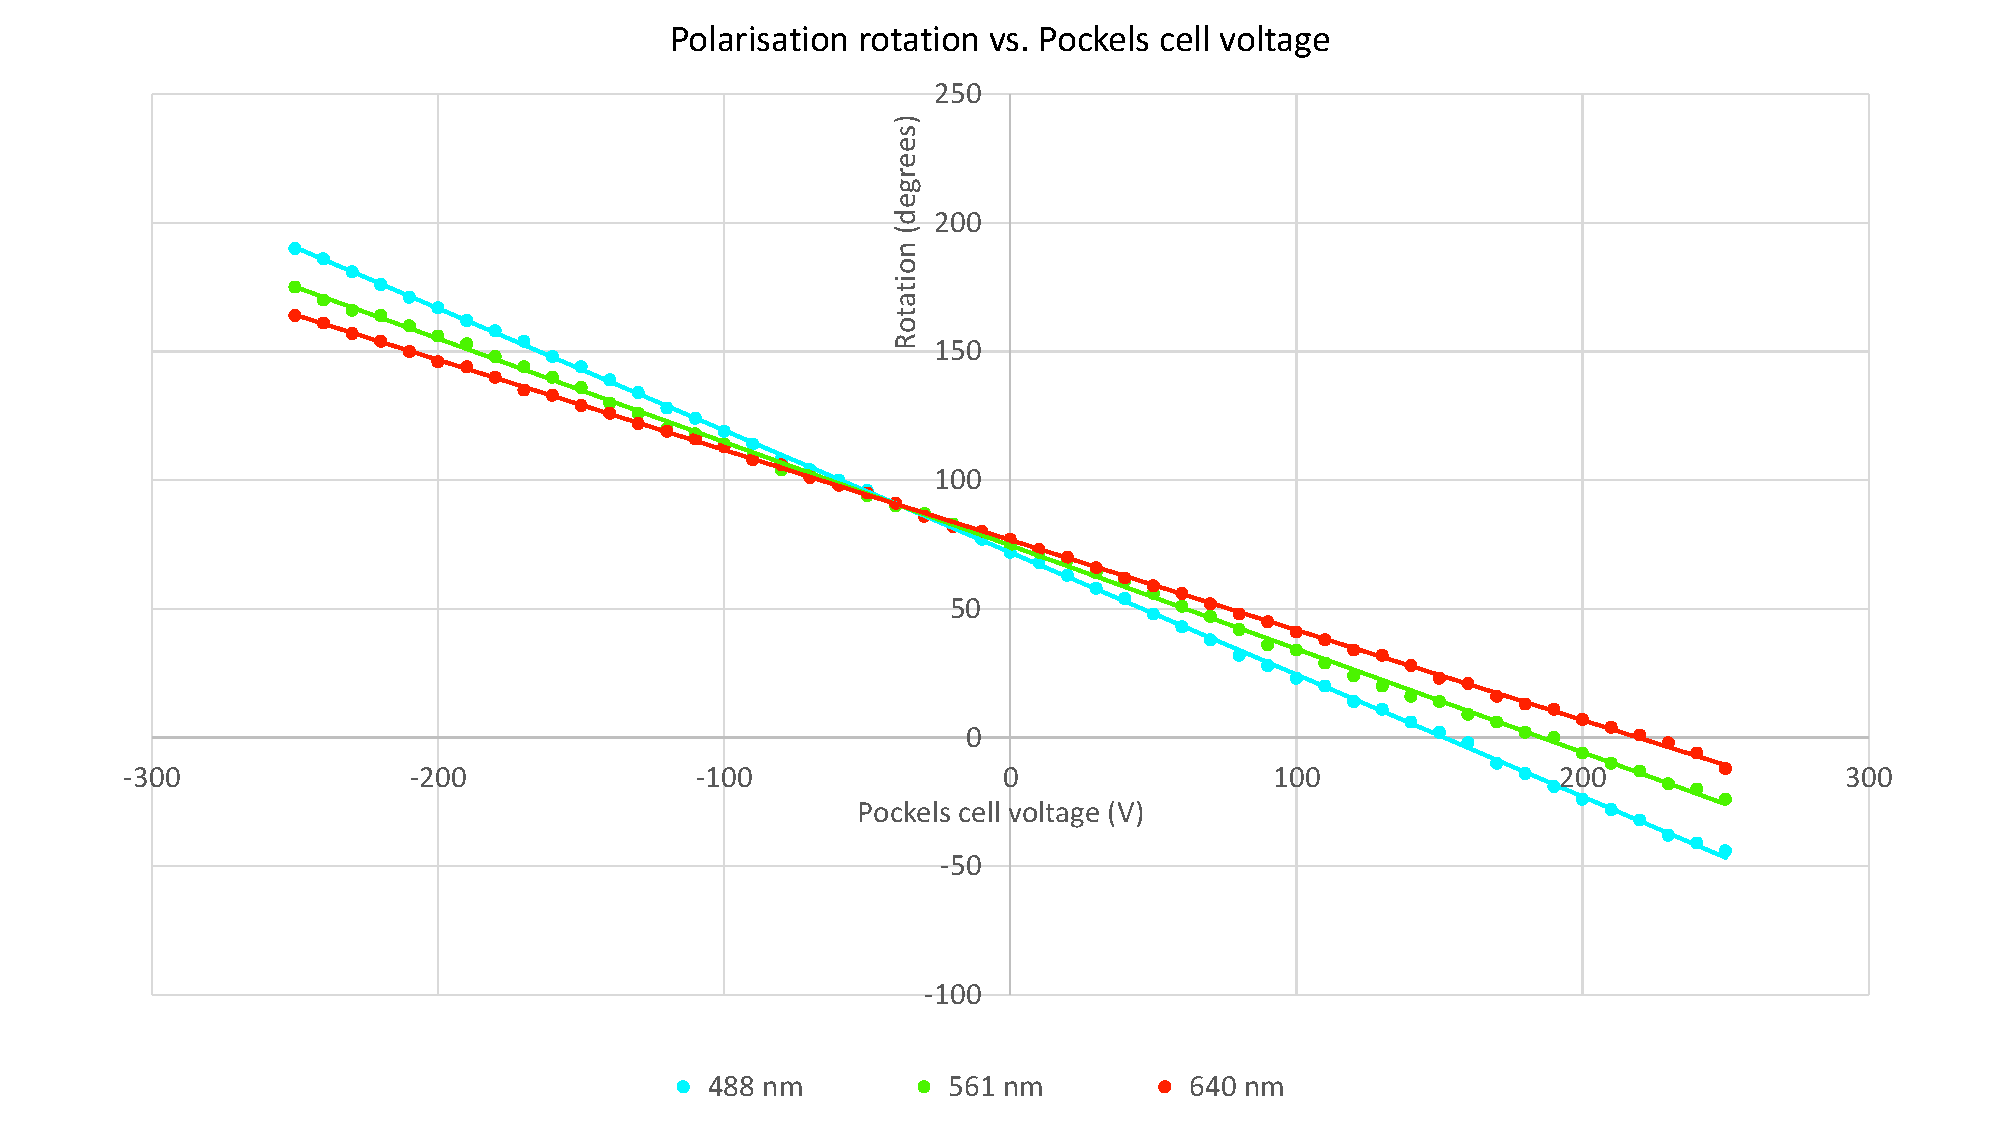
\includegraphics[width=1.0\textwidth]{pockels-voltage-vs-rotation}
\caption[LAG SIM: A Pockels cell is used to rotate the polarisation of laser light for maximum SIM pattern contrast]{When used in combination with a quarter wave plate, the voltage across the Pockels cell is proportional to polarisation rotation for each wavelength of laser light. Though the relationship is slightly different for each wavelength, at low voltages the values are similar enough that the~\SI{561}{\nano\metre} voltages can be used when the Optosplit is employed to image multiple channels simultaneously.}
\label{fig:pockels-voltage-rotation}
\end{figure}

Figure~\ref{fig:pockels-voltage-rotation} shows the relationship between voltage and polarisation rotation for the three laser lines used on the LAG SIM.
Two useful properties of the Pockels cell are evident.
Firstly, the Pockels cell is able to provide a full \SI{180}{\degree} polarisation rotation for all wavelengths, more than adequate for the \SI{\pm60}{\degree} required to align polarisation with the SIM pattern orientations.
Secondly, to achieve a given rotation a similar voltage is required for all wavelengths.

\begin{figure}[p!]
\centering
\begin{subfigure}[b]{\textwidth}
	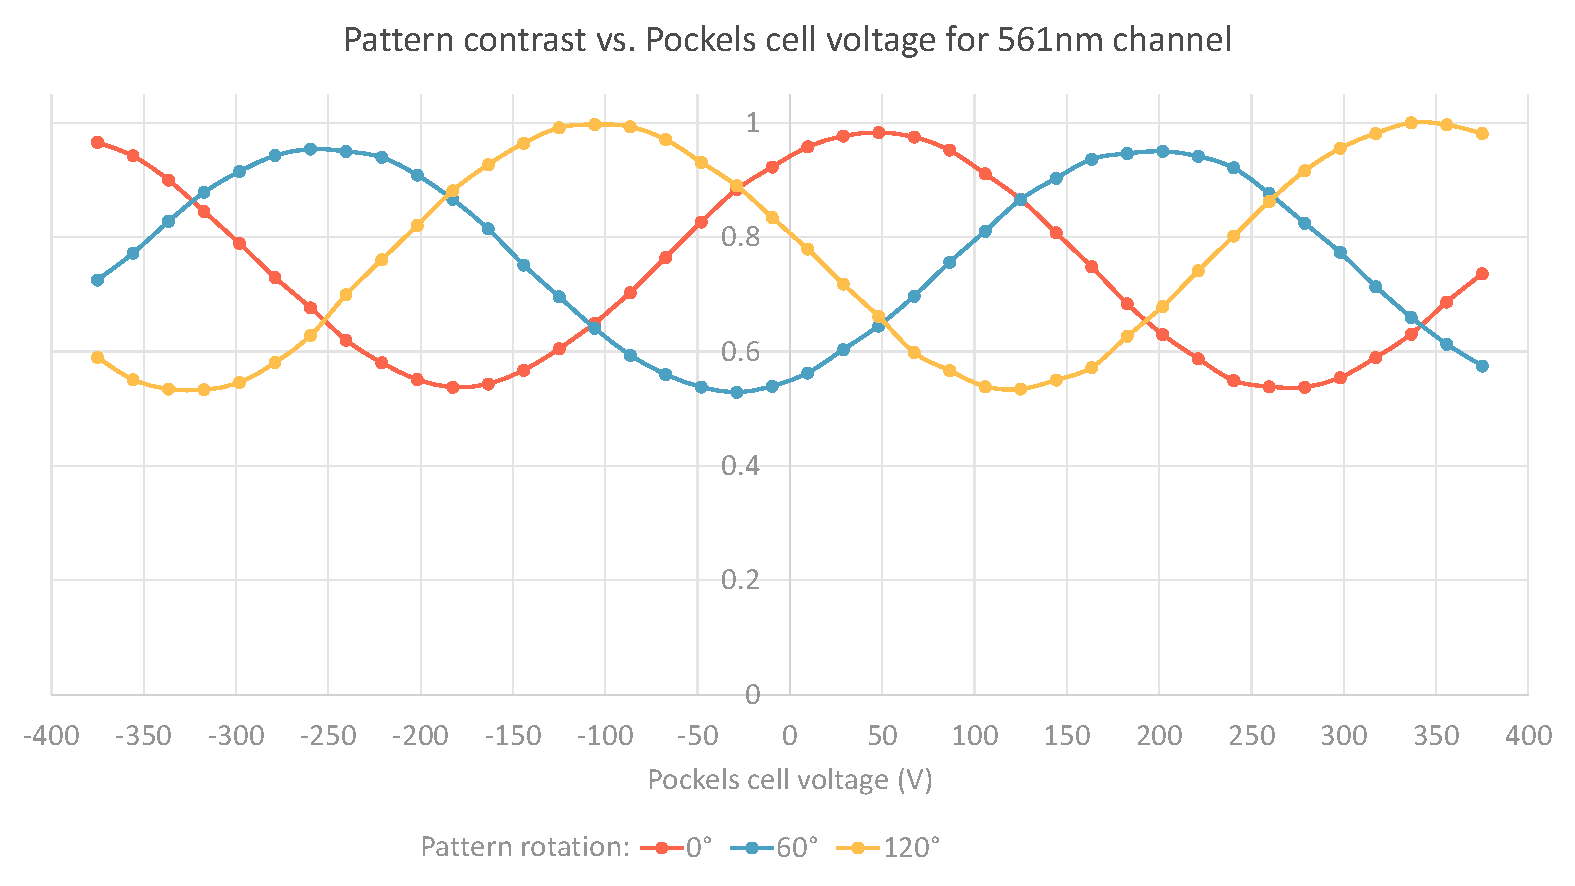
\includegraphics[width=1.0\textwidth]{pockels-contrast}
	\caption{}\label{fig:pockels-contrast}
\end{subfigure}
\begin{subfigure}[b]{\textwidth}
	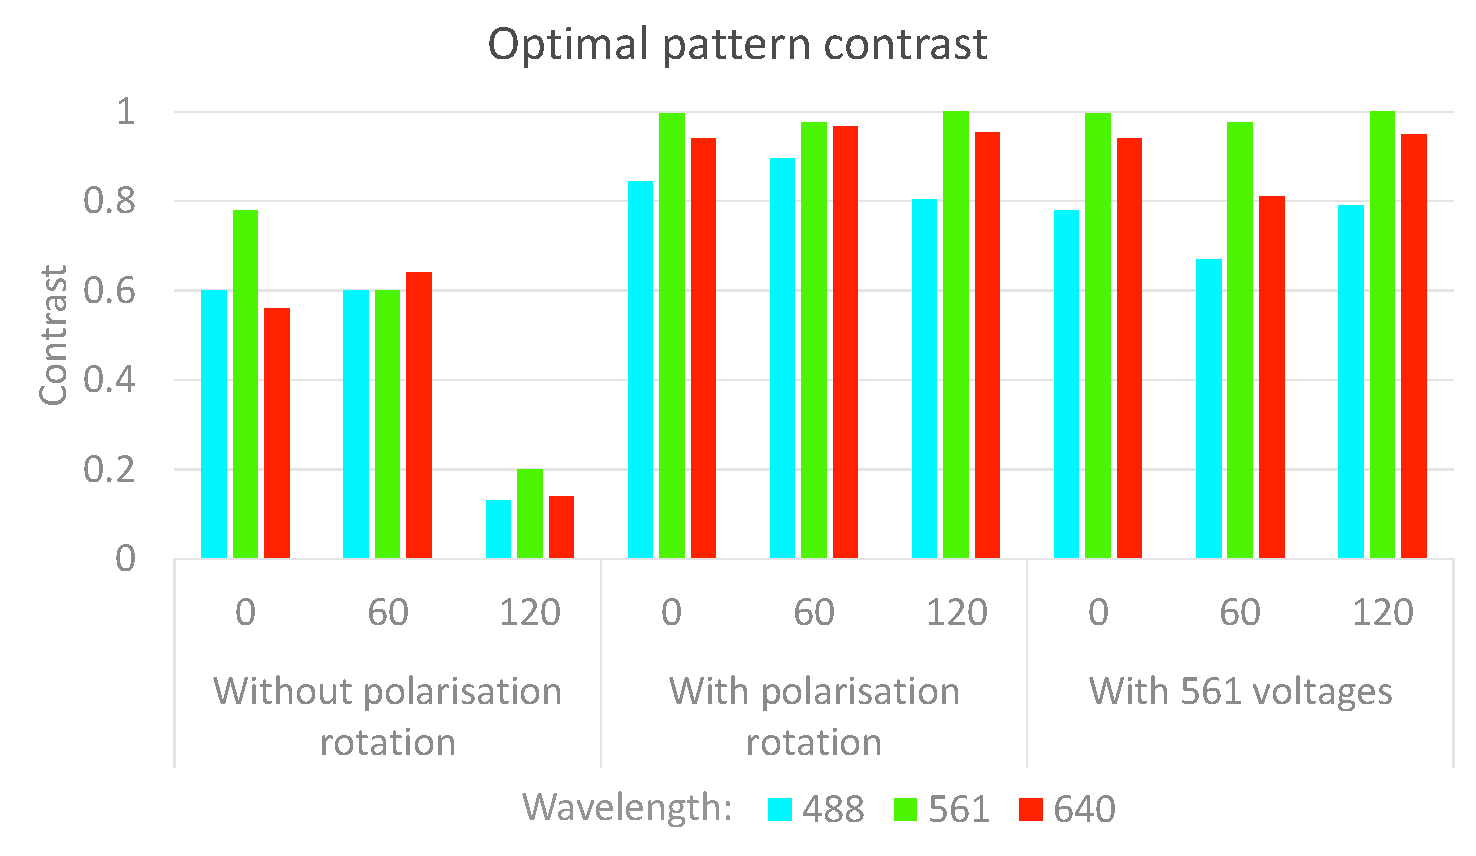
\includegraphics[width=\textwidth]{pockels-rotations}
	\caption{}\label{fig:pockels-optimal}
\end{subfigure}
\caption[LAG SIM: Measurements of a bead sample reveal the optimal Pockels cell voltages for maximum pattern contrast]{(a) shows the pattern contrast, measured on a \SI{100}{\nano\metre} bead sample, as the voltage was swept from \SIrange{-375}{375}{\volt} to find the voltage which gave maximum contrast. The process was repeated for each rotation of the sinusoidal SIM pattern, and for each wavelength of light. (b) shows that rotating polarisation leads to high pattern contrast for all rotations and wavelengths. Furthermore, since the required voltage to achieve a given rotation is similar for all wavelengths, using the \SI{561}{\nano\metre} voltages allows for imaging multiple channels simultaneously whilst maintaining a high pattern contrast.}
\label{fig:pockels-contrast-figures}
\end{figure}
\afterpage{\clearpage}

To measure pattern contrast at a given voltage, images of sub-diffraction beads were recorded under sinusoidal SIM illumination.
Beads located in a trough of the pattern were dark; conversely beads lying in a peak were bright.
At each voltage step the phase of the illumination pattern was swept so that, at some point during the phase sweep, each bead passed through a peak and a trough.
Calculating the difference between the maximum and minimum brightness for each bead provides a measure of pattern contrast for a given voltage.

To calculate the voltages required to achieve maximum pattern contrast at each wavelength and orientation, a LabVIEW program was written to sweep the Pockels cell voltage in steps of \SI{25}{\volt}.
Pattern contrast was measured at each voltage, shown in Figure~\ref{fig:pockels-contrast}.
Each orientation of the illumination pattern has a different voltage which gives a peak contrast.
The optimal pattern contrast measurement was repeated for each pattern orientation at each wavelength, as shown in Figure~\ref{fig:pockels-optimal}.
%The contrast measurement was repeated around each peak to find the optimal contrast voltage to the nearest \SI{1}{\volt}, shown inset on Figure~\ref{fig:pockels-contrast}.

Without polarisation rotation, optimum pattern contrast cannot be achieved, and is almost at a minimum for the \SI{120}{\degree} pattern orientation.
Performing SIM without polarisation rotation would introduce significant artefacts in the reconstruction, as low modulation contrast translates into low signal-to-noise ratio of high frequency components, as described in Section~\ref{sec:SIM-theory}.
Furthermore the signal-to-noise ratio would vary in each orientation, producing an OTF and corresponding PSF which is not rotationally symmetric, adding more artefacts to the reconstructed image.

When the Pockels cell is used to rotate polarisation, a high pattern contrast can be achieved in all orientations of the illumination pattern at each wavelength.
This corresponds to a high modulation depth $m$ in Equation~\ref{eq:matrix-solved}, translating directly into high signal-to-noise ratio for high frequency components and facilitating artefact-free SIM reconstruction with 2$\times$ resolution enhancement.

Furthermore, because the voltages to achieve a given polarisation rotation are similar for all wavelengths, the polarisation of all three laser wavelengths can be rotated simultaneously using the \SI{561}{\nano\metre} optimal voltages.
Figure~\ref{fig:pockels-optimal} shows that a high pattern contrast is still maintained for each wavelength in this scheme.
This facilitates use of the Optosplit for simultaneous 3-channel SIM imaging, providing multicolour resolution enhancement over 6$\times$ faster than capturing channels separately and switching emission filters with a filter wheel.


\section{LabVIEW hardware control} \label{sec:labview}
\subsection{Control requirements for SIM imaging} \label{sec:SIMsteps}
The LAG SIM has a number of hardware components which must all work together to acquire a set of images appropriate for SIM reconstruction.
Specifically, the following sequence of events must take place:
\begin{enumerate}
	\item Set filter wheel to correct position for the excitation and emission wavelengths
	\item\label{step:pockels} Set voltage across Pockels cell for correct polarisation rotation
	\item Set SLM pattern to the correct orientation and phase
	\item Turn on the laser
	\item Open the camera shutter for the exposure time
	\item Close the camera shutter
	\item Turn off the laser
	\item\label{step:record} Record the image
\end{enumerate}
Steps \ref{step:pockels} to \ref{step:record} must be repeated for each of the 9 illumination patterns, and the entire process then repeated for additional colour channels if the Optosplit is not being utilised.
For a time series, this entire process must then be repeated for the required number of frames; for a z-stack, the distance from the stage to the lens must also be adjusted before repeating the process.

The original SIM, detailed in~\cite{young2016guide}, used a separate software program for controlling each piece of hardware.
This caused a number of problems: firstly, setting up experiments was a complicated process prone to human errors, due to the number of parameters which had to be correctly entered in separate programs; and secondly, making modifications to the imaging parameters during an imaging session was difficult and time-consuming.
When imaging live-cell biology, there is a real impetus to image quickly, as cells become unhealthy and soon die on the microscope stage.

Furthermore, the complicated system meant that only one person in the LAG had the knowledge to gather images from the SIM.
This meant that any biological experiments which would benefit from SIM required my direct supervision, so that many projects were not able to use the SIM, and that I personally had little time for my other research aims.
There was a clear need for a new, unified SIM interface, which could be used by non-expert users with minimal training.

\subsection{A user-friendly LAG SIM interface enables operation by non-expert users}
The new interface was built in LabVIEW.
Although each hardware component came with its own control software, all components could also be controlled either through serial commands, analog voltages, or transistor-transistor logic (TTL) levels.
As a graphical language with hardware control in mind, LabVIEW provides easy-to-use built-in blocks to fulfil each of these functions, as well as a clear visual representation of a sequence of control events.
Furthermore it makes designing user interfaces a straightforward process, allowing a programmer to create a user-friendly program for the end user.
This made LabVIEW an ideal candidate for building an accessible program for controlling the LAG SIM.

The LAG SIM interface is shown in Figure~\ref{fig:lagsimLabview}.
The key functions are located in the orange Live Mode area and the blue Acquire tab, although for the sake of completeness each tab is detailed in this section.

\begin{figure}[p]
\centering
\begin{subfigure}[b]{0.6\textwidth}
	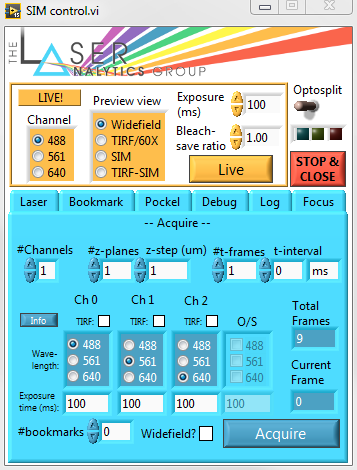
\includegraphics[width=\textwidth]{lagsimLabviewAcq}
	\caption{}\label{fig:fpbLabviewAcq}
\end{subfigure}

~\newline
\begin{subfigure}[b]{1.0\textwidth}
	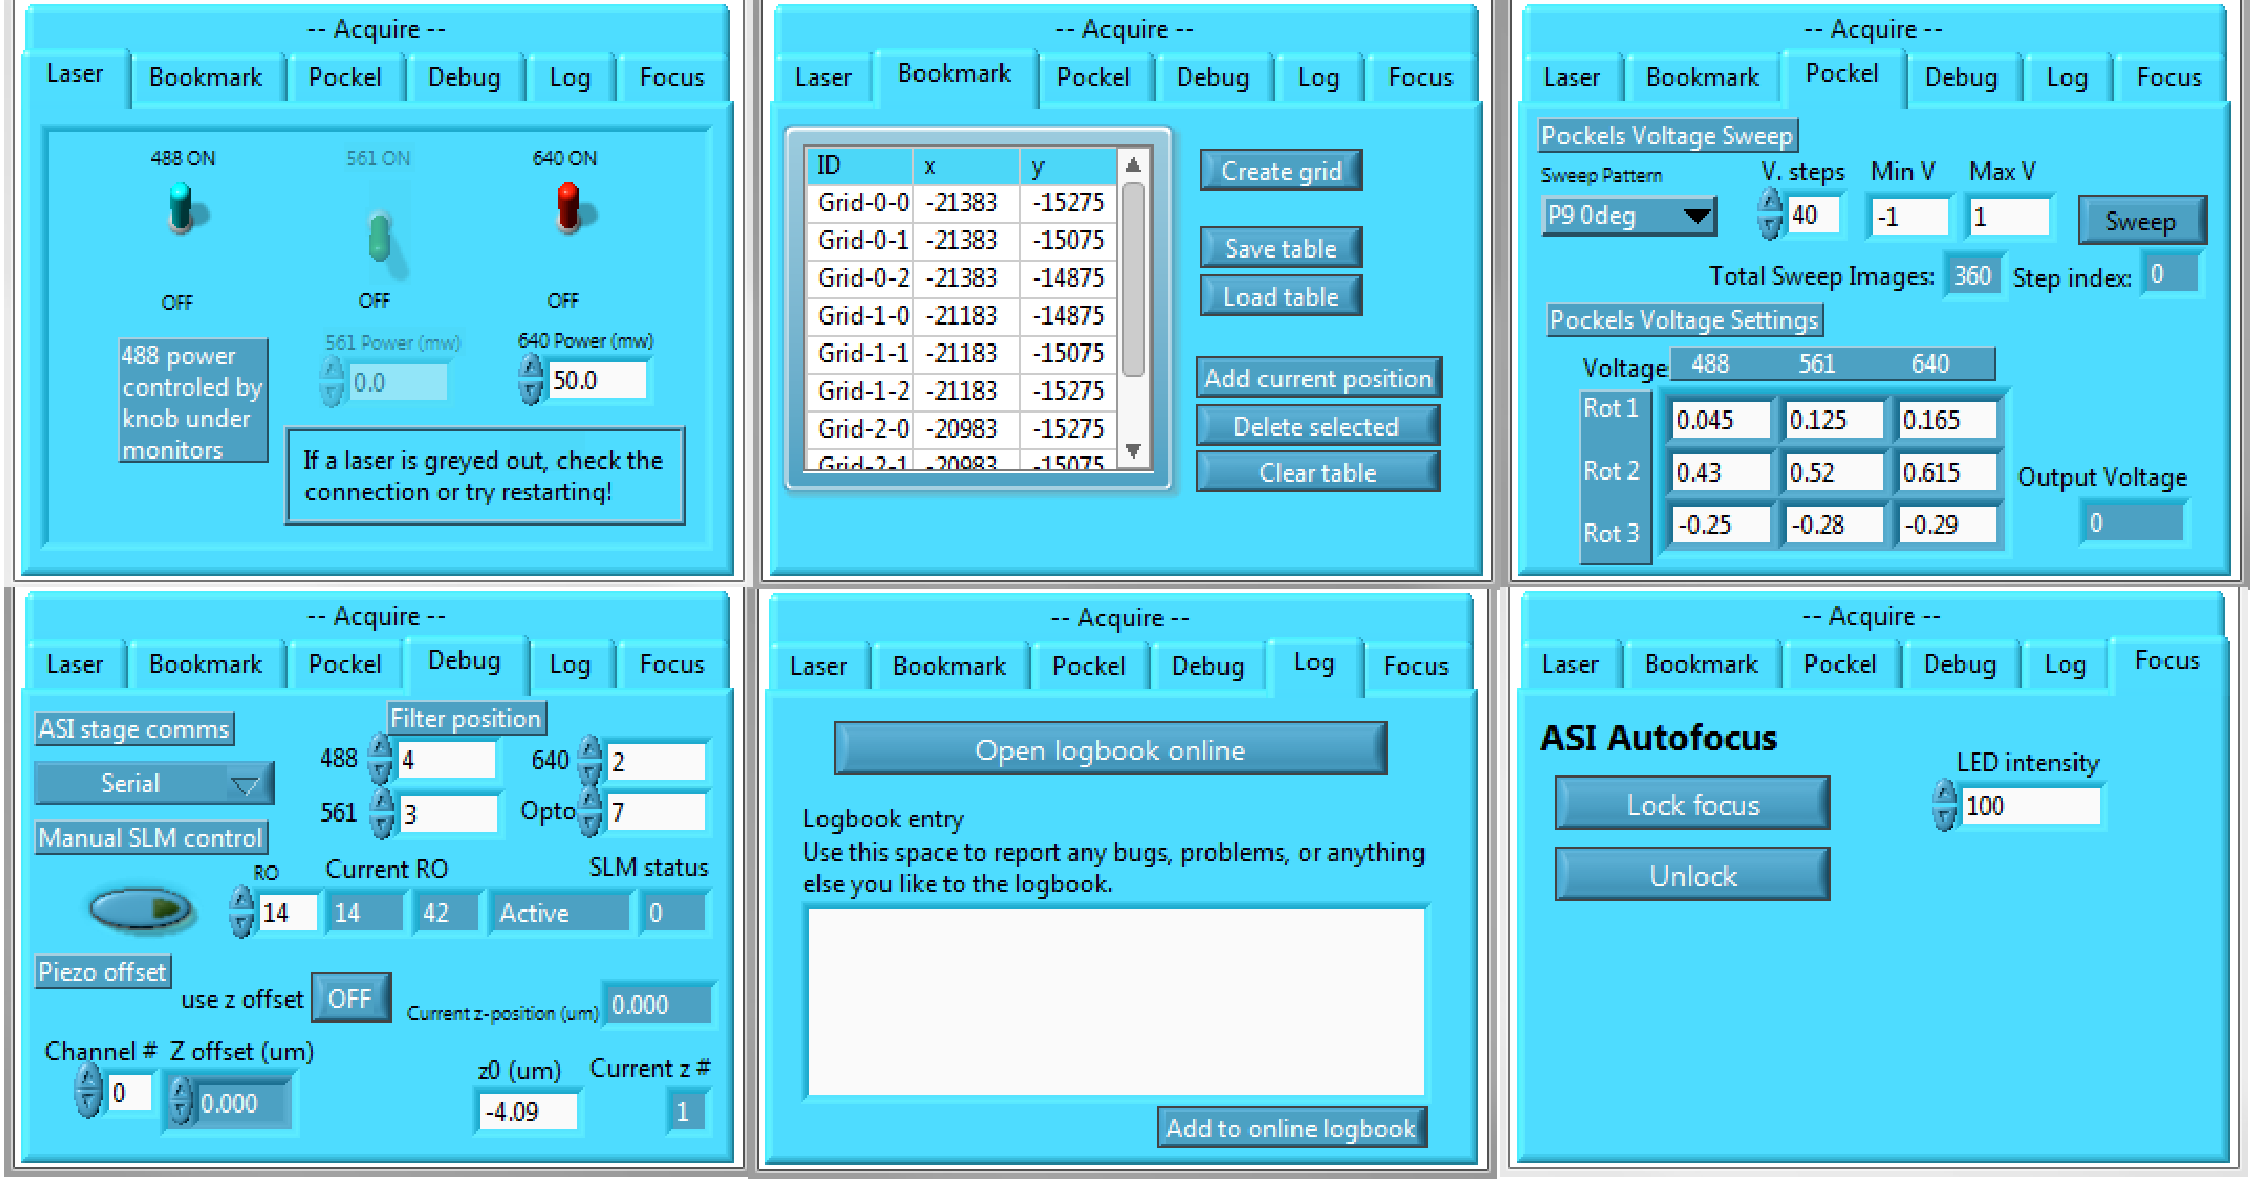
\includegraphics[width=\textwidth]{lagsimLabviewOthers}
	\caption{}\label{fig:fpbLabviewTabs}
\end{subfigure}
\caption[LAG SIM: The LabVIEW user interface for controlling LAG SIM is designed for operation by non-expert users]{The LabVIEW user interface used to control the LAG SIM has been designed for operation by a non-expert user, with advanced tasks hidden in the extra tabs shown in (b). } % Needs a few more words actually
\label{fig:lagsimLabview}
\end{figure}

\subsection{Live tab for fast image preview} \label{sec:lagsimLive}
The live tab is always visible whenever the LAG SIM control software is open.
It works in conjunction with the HCImage camera software provided by Hamamatsu, which provides a live display of the camera chip.

In live mode, the illumination wavelength can be changed with the radio buttons or with the F2, F3 and F4 keys for fast, mouse-free operation.
This allows users to quickly identify cells in one channel, for example with a fluorescent nucleus marker, and confirm presence of another marker in the second channel.
This fast channel switching minimises photobleaching when panning for healthy cells to image in detail.
% This is surprisingly useful, see supplementary video?

Another live-mode feature designed to reduce bleaching is the so-called `bleach-save ratio.'
This is a number between 0 and 1 which switches off the laser for a fraction of the exposure time.
By setting the exposure time and bleach-save ratio as small as possible while still being able to find healthy cells, the level of light the sample is exposed to can be minimised.
This is especially important in live-cell biology, where excess light can cause phototoxic effects bringing about cell death.

The illumination pattern used for live mode will usually be a pseudo-widefield mode, which emulates widefield illumination by dithering all three phases of a SIM pattern over one exposure time of the camera.
True epi-illumination is not possible on the LAG SIM due to the spatial mask, which blocks the 0-order diffraction spot in the Fourier plane.
The user can also choose to preview the SIM pattern by selecting the appropriate radio button; if the stripe pattern is visible, this is a good indication that later reconstruction into a resolution-enhanced image will be successful.
If the \SI{1.49}{\numaperture} TIRF lens is used, then selecting the TIRF radio button sets the SLM pattern such that the ±1 diffraction spots hit the TIRF ring on the objective back aperture, leading to TIRF illumination at the sample.
This can be done with the SIM pattern visible or in a dithered mode, as with non-TIRF illumination.

The Optosplit rocker in the control software sets the system up for imaging with the Cairn Optosplit III.
The Optosplit is a device on the output port of the microscope which contains two filter cubes and a set of mirrors so that each channel can be imaged simultaneously onto a separate 512$\times$512 area of the 2048$\times$2048 camera chip.
When the filter cubes are removed, and the Optosplit rocker is in the \texttt{OFF} position, the Optosplit has no effect and channels are imaged sequentially, with an appropriate filter for each channel loaded into position by the filter wheel.
With Optosplit mode \texttt{ON}, however, the live-mode channel selection radio buttons become checkboxes, so that each colour channel can be switched on and off independently.
The Optosplit provides much faster imaging speeds, at the potential cost of cross-talk between colour channels.

% Should actually move most of this up? and just talk about the user interface here, maybe about assessing bleedthrough from shorter wavelengths to longer ones

This upper section of the user interface contains two more important components.
A laser status indicator shows which lasers are currently exposing, an important safety feature so that users know it is safe to remove their sample after an imaging session.
The \texttt{STOP \& CLOSE} button safely exits the control software, ensuring that the lasers are switched off, the camera is finished exposing, and the voltage across the Pockels cell is set to \SI{0}{\volt}.
To ensure that this exit sequence runs when a user has finished their imaging session, the $\times$ close button in the window's title bar is disabled.

\subsection{Acquire tab facilitates multi-dimensional imaging}
Once a healthy cell with the required staining has been located from live mode, it can be captured as a SIM image with the Acquire tab.
With the default settings shown in Figure~\ref{fig:fpbLabviewAcq}, this will capture a set of 9 raw SIM images following the steps described in Section~\ref{sec:SIMsteps}.
Additional settings in this tab allow a set of images to be captured for 3D z-stacks, timelapse imaging, and other multi-image acquisitions.

If the number of \texttt{z-steps} is greater than 1, then the ASI stage will move in the axial direction at the end of every SIM acquisition by the value given in the \texttt{z-step} box.
Since the axial resolution of the SIM is \SI{440}{\nano\meter}, for a Nyquist-limited z-stack a \texttt{z-step} of \SI{200}{\nano\meter} should be used.

To take a series of images over time, the \texttt{t-frames} parameter should be set to greater than 1.
For observing fast, dynamic events, the \texttt{t-delay} parameter should be set to \SI{0}{\milli\second}.
Timelapse imaging, for example capturing an image every minute for an hour, can be achieved by setting the \texttt{t-delay} to \SI{60}{\second}, which will pause the software for the given amount of time at the end of each acquisition.

Multi-channel imaging can be achieved either with or without the Optosplit.
If the Optosplit switch is set \texttt{OFF}, and the number of channels is set to more than 1, the filter wheel will rotate the correct filter into position after each channel is captured.
The exposure time of each raw SIM frame can be set per-channel, and the channel order can be changed with the radio buttons.

Faster imaging can be achieved with the Optosplit.
This sets the filter wheel to an empty filter, and filtering is performed with filter cubes in the Optosplit.
In this mode, the choice of channels is controlled with checkboxes.

The bookmarks number should be set to the number of bookmarks in the bookmarks table, or a lower number $N$ if the user only wants to capture the first $N$ bookmarked locations from the table.
If bookmarks are not to be used, this value should be left at 0 - a value of 1 will move to the first bookmark listed in the bookmark table and capture an image there.
Bookmarks are discussed in more detail in Section~\ref{sec:lagsimBookmarks}.

The LAG SIM microscope can be used to capture images in a pseudo-widefield mode, by dithering the SIM pattern as described in Section~\ref{sec:lagsimLive}.
This is enabled by ticking the \texttt{Widefield} checkbox.
This will enable imaging with widefield resolution at the camera's maximum acquisition speed of \SI{100}{\hertz}.

Once the appropriate variables have been set for the acquisition, the total frames is displayed in the \texttt{Total frames} box.
This number should be entered into the HCImage camera software, to prepare the camera for a high-speed image acquisition.
Once the user has pressed \texttt{Start} in the HCImage software, the camera buffer is ready to receive images; then pressing \texttt{Acquire} in the LAG SIM software starts the acquisition process.

A future version of the software could automate this final step, eliminating the need for the HCImage software.
This would require synchronised access to the camera data stream through LabVIEW.


\subsection{Laser tab provides safe power control}
Laser control is integrated into the LAG SIM control software.

At the launch of the software, the controls are greyed-out and disabled.
When LabVIEW successfully connects to each laser, its controls become enabled, to switch the lasers on and off and change the power.
Lasers are switched off automatically when the software is closed, for added safety when the microscope is unattended.

Having fast and straightforward access to laser control is particularly useful for reducing light dosage in live mode.
Power can then be increased for acquisition to obtain the highest possible image quality.

\subsection{Bookmark tab for saving positions and creating mosaics} \label{sec:lagsimBookmarks}
The LAG SIM LabVIEW program is able to store locations on the microscope slide as bookmarks.
If the number of bookmarks in the \texttt{Acquire} tab is set to greater than 0, the microscope stage will move before each acquisition to the next bookmarked position in the bookmark table.
This is especially useful for imaging a collection of cells over a long period of time.

The SIM user can pan around the microscope slide in \texttt{Live} mode searching for healthy cells with good fluorescent labelling, and save them to the bookmark table by clicking \texttt{Add bookmark}.
The location can be returned to by double-clicking on the table entry, or acquired sequentially and repeatedly in the \texttt{Acquire} tab.

Furthermore this tab contains an option for creating bookmarks in a grid pattern.
This can be utilised for imaging large areas, which are then stitched together to form one large mosaic image, for example the whole mouse brain shown in Figure~\ref{fig:wholebrain}.

\begin{figure}[p]
\centering
\includegraphics[angle=90, width=1.0\textwidth]{whole-brain}
\caption[LAG SIM: An image of a full mouse brain can be captured as a mosaic of images]{The bookmark mode offered by LAG SIM can be used to create tiled images, such as this 3-colour image of a mouse brain. Dissection and staining performed by Sarah F{\"o}rster. Scalebar is \SI{500}{\micro\metre}.}
\label{fig:wholebrain}
\end{figure}

\subsection{Focus tab controls the autofocus} \label{sec:lagsimFocus}
Using the grid bookmark function to image large fields of view can fail if the coverglass or microscope stage is not perfectly flat, which is often the case in practical experiments.
To keep the focus locked at the same distance from the sample, the `Lock focus' button begins the autofocus procedure.
Assuming the autofocus sensor receives enough reflected signal from the infrared autofocus light emitting diode (LED), the sample will be locked at a fixed distance from the objective lens.
If not, an error message is returned requesting the user to increase the LED power for a stronger signal.
The system can also be used to maintain focus over a time period of hours to days, even as the objective lens drifts away from the sample.

The autofocus is switched off with the `Unlock focus' button, releasing z-control back to the user.

\subsection[Pockels tab to find optimal voltages for maximum pattern contrast]{Pockels tab to find optimal voltages for maximum pattern\\ contrast}
The Pockels cell retards one polarisation axis by an amount dependent on the voltage across it.
In combination with a quarter wave plate, this allows for linear polarisation rotation necessary for the high pattern contrast required for SIM, explained in Section~\ref{sec:lagsim-pockels}.
The amount of retardation depends on the wavelength of light, therefore different wavelengths require different voltages to achieve the same polarisation rotation.

To find the optimum voltage for each wavelength, functionality is implemented in the \texttt{Sweep} tab to sweep the voltage from \SIrange{-1}{1}{\volt}, in a number of voltage steps.
At each voltage, the SIM pattern's phase is swept and pattern contrast can be measured using a diffraction-limited bead sample.
Pattern contrast is calculated with a MATLAB script to produce the graph in Figure~\ref{fig:pockels-contrast}, showing how pattern contrast changes with voltage.

This gives a coarse estimation of the voltage required to achieve maximum pattern contrast.
The sweep limits can then be adjusted to a small amount either side of the coarse estimation's maximum contrast to obtain a more accurate voltage.

This process must be repeated for each wavelength, and each rotation of the SIM pattern.
Once the process is complete, the optimum voltages can be entered into the table, and will be applied to the Pockels cell during a SIM acquisition.


\subsection[Debug tab contains alignment options and other advanced features]{Debug tab contains alignment options and other advanced\\ features}
A number of advanced user options are contained in the \texttt{Debug} tab.
These extend the functionality of the microscope for non-conventional uses including alignment.

The emission filters in the filter wheel switch with excitation wavelength for use with commercially available fluorophores.
However, some samples - such as semiconducting perovskites - emit around \SI{750}{\nano\metre} when excited with \SI{488}{\nano\metre} light.
Unconventional filters can be selected in this tab to image these samples.

Manual SLM control gives the user direct control over the pattern displayed on the SLM.
This means specialised patterns, such as a SIM pattern masked by a circle, or even 3 SIM patterns with different orientations overlayed, can be used.
These types of patterns are particularly useful for alignment of the system: overlaying 3 orientations of the SIM pattern produces 6 spots at the Fourier plane, which must be centred around the optical axis; therefore a coarse alignment can be performed using a translucent pinhole alignment tool on the microscope, as shown in Figure~\ref{fig:pinhole-alignment}.
A fine alignment is then performed using the masked patterns, by ensuring the two circles overlap at the focal plane of the microscope~\cite{young2016guide}.

\begin{figure}[htbp!]
\centering
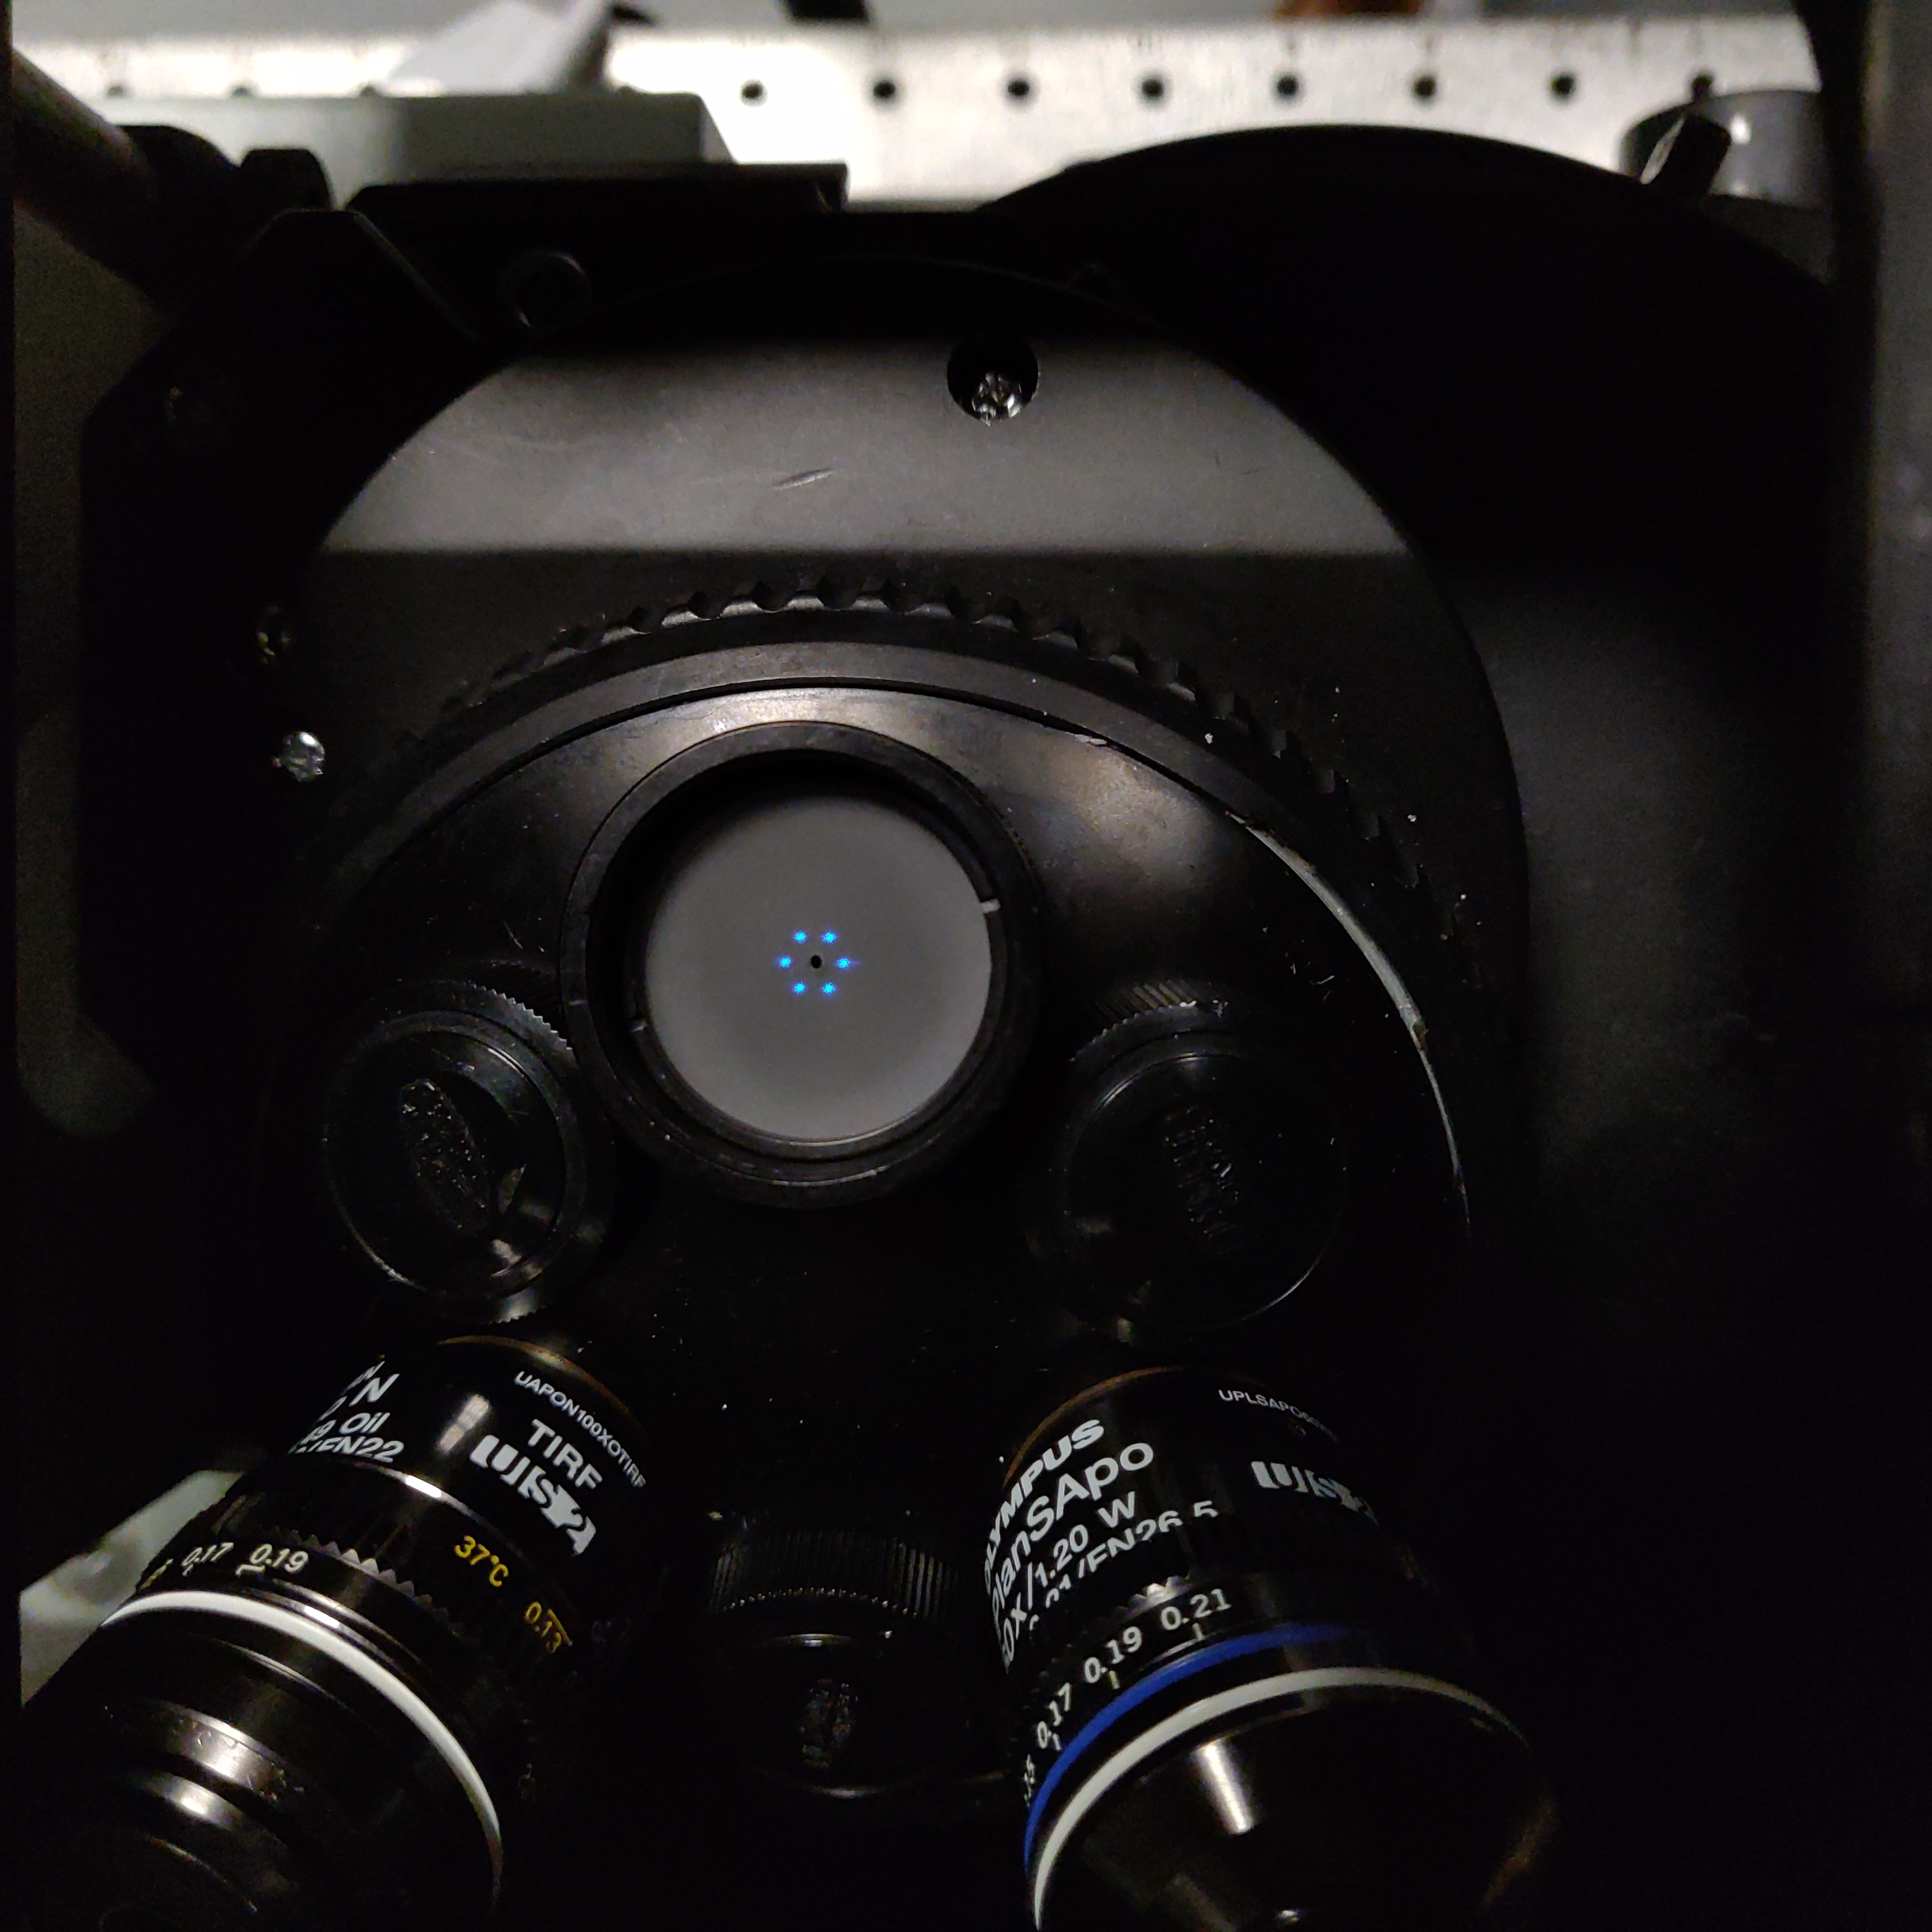
\includegraphics[angle=-90, width=0.6\textwidth]{sim-alignment}
\caption[LAG SIM: Displaying specially designed patterns on the SLM assists with alignment of LAG SIM]{The 3 orientations of the SIM pattern are overlaid on the SLM, such that 6 spots are produced in the Fourier plane for alignment. The spots should be aligned such that the pinhole is at the centre of the spots.}
\label{fig:pinhole-alignment}
\end{figure}

Finally, the \texttt{Piezo Offset} section adjusts the z-position of the stage for each channel to account for chromatic offset.
In practice this offset is less than \SI{100}{\nano\meter} and \texttt{Piezo Offset} is only used for maintaining correct focus in TIRF imaging.

\subsection{Log tab provides access to an online logbook}
The LAG SIM control software logs all activity automatically to Labstep, an online laboratory management system~\cite{labstep} shown in Figure~\ref{fig:labstepTimeline}.

When a user opens the LAG SIM software, they are asked to enter their name for the online logbook.
When they press \texttt{Start}, the software sends an HTTP request to a Labstep timeline,  recording the user's name and the start time.
Similarly, when they \texttt{Stop \& Close} the software, their name and finish time is logged to the timeline, along with any errors generated by the software during their use.

Furthermore, every acquisition is also logged to the timeline.
This contains metadata relating to the acquisition, for example number of \texttt{t-frames}, \texttt{z-steps}, laser powers, and exposure times.
This is especially helpful is the user is later unsure what acquisition parameters were used for a particular image.

The user can also add a customised post to the logbook, for example to record an error with the software.
The online Labstep logbook can be opened by clicking the \texttt{Open logbook} button, opening the webpage shown in Figure~\ref{fig:labstepTimeline}.

\begin{sidewaysfigure}[p]
\centering

\includegraphics[width=0.875\textwidth]{labstep-timeline}
\caption[LAG SIM: Logging user activity with Labstep allows any problems to be identified and fixed quickly]{User activity is automatically logged to an online logbook hosted on Labstep to identify and fix any problems quickly. This figure shows the user logged onto the SIM at 09:00, acquired 2 images - a SIM z-stack then a 1000-frame widefield video - then logged off.}
\label{fig:labstepTimeline}
\end{sidewaysfigure}

Online logging benefits both the microscope user and the developer, allowing problems to be identified and fixed promptly.

\clearpage
\section{A comparison of reconstruction algorithms reveals their pros and cons} \label{sec:recon}
Once SIM data is collected, it requires reconstruction to either enhance the resolution, remove out-of-focus light, or a mixture of both.

A basic SIM reconstruction algorithm implements the following steps:
\begin{enumerate}
	\item Extract illumination pattern parameters (orientation angle and phase shift)
	\item Separate Fourier space images into individual frequency components
	\item \label{step:filterPreShift}Weight components in Fourier space by OTF and filter for noise removal
	\item \label{step:shiftComponents}Shift frequency components into correct position in Fourier space
	\item Perform inverse Fourier transform to obtain the reconstructed image
\end{enumerate}

Additional steps are often added into the basic algorithm to reduce artefacts.
Raw images may be corrected for consistent intensity and contrast across the dataset, and an additional filtering step for noise removal can be applied before the images are separated in Fourier space.
Note also that step \ref{step:filterPreShift} can be performed after step \ref{step:shiftComponents}, but this can lead to additional artefacts in the reconstructed image~\cite{gustafsson2008three}.
Artefacts can furthermore be suppressed by apodisation before the final inverse Fourier transform~\cite{gustafsson2008three}.

This basic algorithm will provide resolution enhancement, but does not implement optical sectioning for removing out-of-focus light.
This requires an additional attenuation step, applied simultaneously with step \ref{step:filterPreShift}.

Various implementations of the SIM reconstruction algorithm exist.
During the course of my PhD, I have utilised and modified three different reconstruction algorithms, and written a plugin for ImageJ tailored specifically for LAG SIM and detailed in Section~\ref{sec:lagsimFiji}.
Each implementation has its own merits and disadvantages, discussed in the remainder of this section.

\subsection{Lin Shao SIM reconstruction runs on CUDA GPUs}
The first implementation of the resolution-enhancing SIM algorithm used in the Laser Analytics Group was provided by Lin Shao, who worked on SIM with Mats Gustafsson~\cite{shao2011super}.
It was developed during his time at Janelia Farm Research Campus, under the supervision of Gustafsson and Eric Betzig~\cite{beach2014nonmuscle}.

Shao's algorithm is written in native CUDA code, a programming model for parallel computation with Nvidia graphics cards~\cite{sanders2010cuda}.
This makes reconstruction very fast - around 1 frame per second on an Nvidia Quadro 2000.
However, native CUDA must be recompiled from source on every new computer it is used on, and furthermore because the software has not been updated, it does not work with the latest version of CUDA.

The program has no graphical user interface, but is called from the command line.
Command line calls can be made from most other programming languages, so a custom interface was built in MATLAB to make reconstruction a simpler process.
The MATLAB interface firstly separates complex datasets such as multi-channel z-stacks into individual SIM frames, and sends these along with the correct reconstruction parameters, based on the lens used, to the command line reconstruction program.
An example command-line call is shown in Snippet~\ref{snip:matlab-command}, showing the various input parameters sent as arguments to the compiled CUDA program. 

\begin{lstfloat}
\begin{lstlisting}[language=matlab,caption={Lin Shao's CUDA reconstruction program is executed as a command line program through a MATLAB interface},label={snip:matlab-command},frame=single]
command = ['C:\Users\user\Desktop\SIM\Reconstruction\cudaSIrecon\cudaSireconDriver.exe' ...
    ' --input-file=.\' outname '.mrc' ...
    ' --output-file=.\' outname '_recon.mrc' ...
    ' --otf-file=C:\Users\user\Desktop\SIM\Reconstruction\cudaSIrecon\' otf_file '.mrc'...
    ' --nphases=3'...
    ' --angle0=1.5708'...
    ' --ls=' num2str(linespacing)...
    ' --na=' num2str(na)...
    ' --nimm=' num2str(n_im)...
    ' --zoomfact=' num2str(zoom_factor)...
    ' --wiener=' num2str(wiener)...
    ' --otfRA=1'...
    ' --dampenOrder0=0'...
    ' --nosuppress=0'...
    ' --nokz0=0'...
    ' --k0searchAll'...
    ' --background=100'...
    ' --equalizet=1'];
[status,cmdout] = system(command,'-echo');
if status ~= 0
    error('cudasirecon failed');
else
    save([outname '_info.mat'], 'cmdout')
end
\end{lstlisting}
\end{lstfloat}


Shao's algorithm does not implement OTF attenuation, which is used for optical sectioning.
This means it cannot remove out-of-focus light, so is not appropriate for reconstructing 3D image stacks.

The program was not built for widespread distribution, and as such there is no documentation or publication for it.
Nor is the program publicly available; requests for a copy of the software have to be made directly to Lin Shao.
This means the software is complicated to use, and has not been tested and verified by the wider community.

Lin Shao is now at Yale University; although he is contactable, he is not actively maintaining this piece of software.
Since this implementation is fast becoming obsolete, it is now only installed on one computer in the Laser Analytics Group, which cannot have graphics updates installed.

\subsection{SROS-SIM facilitates optical sectioning}
SROS-SIM is a SIM reconstruction program by Florian Str{\"o}hl which implements both optical sectioning and resolution enhancement.

SROS-SIM is a MATLAB implementation of the super-resolution optical-sectioning (SROS) algorithm detailed by O'Holleran and Shaw in 2014~\cite{oholleran2014optimized}.
Optical sectioning removes out-of-focus light, so that 3D images can be reconstructed, for example of a whole cell with mitochondria labelled as shown in Section~\ref{sec:showcase-MOF}.

As a set of MATLAB scripts and functions, the code can be executed on any computer with a MATLAB license.
Therefore the implementation is available for all major desktop operating systems, and furthermore is easy to modify.
I have made modifications to the original code to perform operations on the graphics processing unit (GPU), bringing a 20$\times$ increase in reconstruction speed.
% Want to show a table of this??

SROS-SIM has the disadvantage of not being publicly available or published and verified by the community.
Furthermore the need for an expensive MATLAB license limits who can use the software.
Finally, the important step of measuring the illumination pattern parameters is not fully automated, so that the software always requires some user input and can cannot be left to run unsupervised for a batch reconstruction task.

\subsection{fairSIM allows reconstruction in ImageJ}
fairSIM is an open-source plugin for ImageJ/Fiji, a popular image analysis suite which is also open source and free~\cite{muller2016open, schindelin2012fiji}.
The software is well-documented and hosted on Github, so it is continually updated and improved by the community.

The fairSIM reconstruction algorithm implements resolution enhancement and optical sectioning, with two different noise filters.
It provides the user with complete control over the input parameters, and with debugging options enabled will show detailed visual output at each stage of the reconstruction.
Although the number of options can be overwhelming for some users, it is powerful and useful software for advanced SIM users.

The fairSIM user interface is cumbersome, and reconstruction can only be performed on a single-colour, single-frame SIM image.
This process requires around 20 clicks, and input parameters must be resubmitted for every reconstruction.
This, coupled with the fact that fairSIM does not have GPU support, makes reconstruction very slow, especially for large, multicolour image sets.

% Hessian SIM?

\subsection{LAG SIM is specifically designed for our microscope}
LAG SIM is my personal implementation of the SIM reconstruction algorithm, built using the well-documented fairSIM Java library~\cite{fairsimGithub}.
It is designed specifically for the Laser Analytic Group's SIM, simplifying the interface for non-advanced users, and implements a fast parameter-finding technique.

It is available publicly as an ImageJ/Fiji plugin~\cite{lagsim}.
This means that it is free, open source, and stays up-to-date for all users.

The next section describes the LAG SIM plugin in detail, providing a detailed resource to anyone reconstructing LAG SIM data in the future.


\section{Reconstruction with LAG SIM for artefact-free images} \label{sec:lagsimFiji}

\subsection{The LAG SIM ImageJ interface simplifies parameter-finding for non-expert users}

Setting SIM reconstruction parameters, particularly for noise filtering and optical sectioning, is a difficult task for new users.
In LAG SIM, which uses the same reconstruction algorithm as fairSIM, there are 3 filter parameters; 2 apodisation parameters; 2 attenuation parameters; and a choice of 2 filters, which can be used in combination.
This makes a high-dimensional parameter space to optimise over.
Selecting appropriate values for these parameters requires understanding what each is for; setting optimum values requires experience and expert skill.

LAG SIM provides a number of tools designed to assist with common SIM reconstruction tasks, reducing the time required between acquisition and analysis of the data.
The tools are accessed through the ImageJ menu shown in Figure~\ref{fig:lagsim-fiji-interface}a.

\begin{figure}[b!]
	\centering
		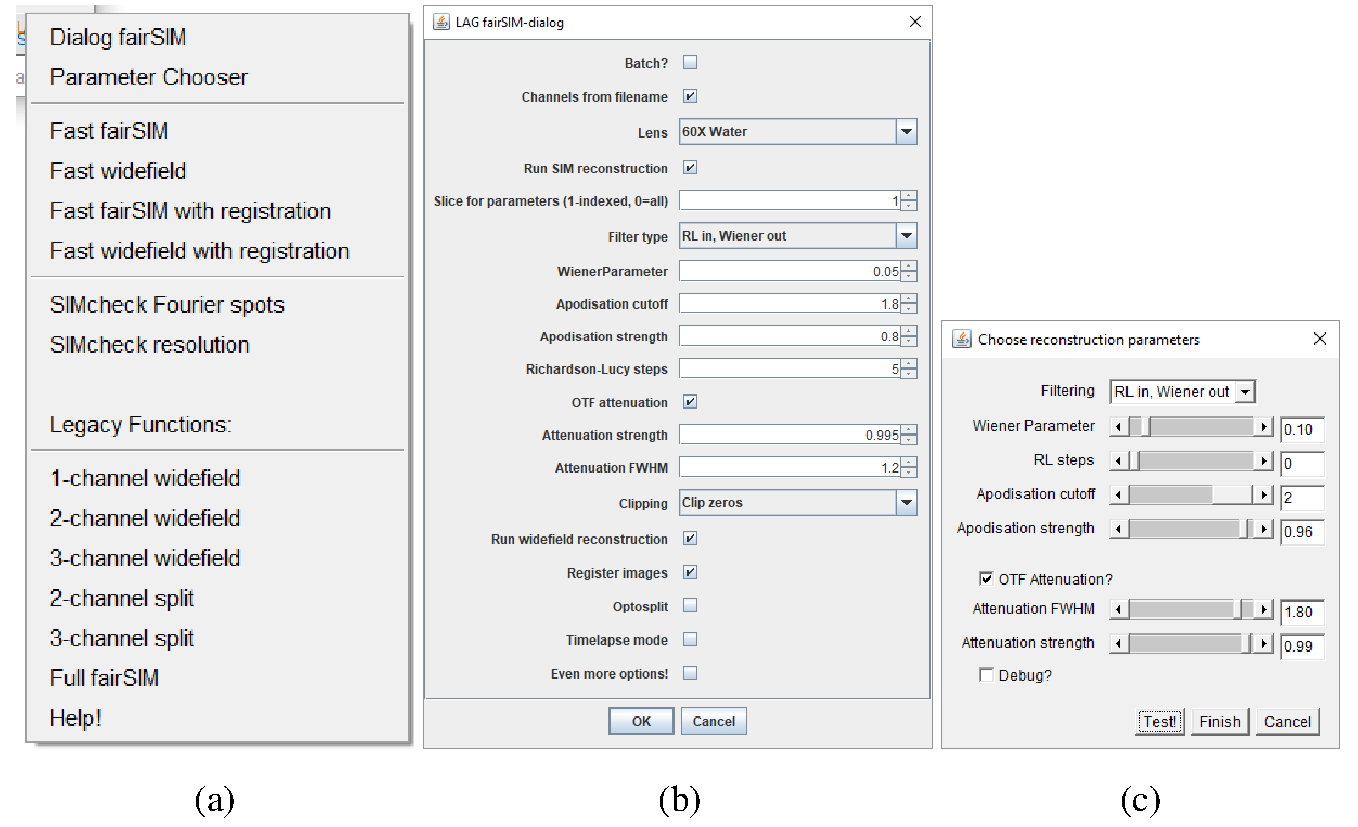
\includegraphics[width=1.0\textwidth]{lagsim-fiji}
	\caption[LAG SIM: A Fiji interface makes artefact-free reconstruction quick and simple for non-expert users]{The LAG SIM ImageJ/Fiji user interface, utilising the fairSIM reconstruction algorithm, is specifically designed for the LAG SIM to make artefact-free reconstruction quick and straightforward. (a) shows the main LAG SIM menu, with the many reconstruction and SIMcheck tools created; (b) shows the quick parameter tester, for finding the optimal reconstruction parameters; and (c) shows the main reconstruction interface, facilitating batch reconstruction. }
\label{fig:lagsim-fiji-interface}
\end{figure}

The ``Fast widefield'' function performs a simple pixel-by-pixel sum across the 9 raw images in each SIM acquisition.
As described in Section~\ref{sec:sim-background}, this simply reconstructs a widefield view of the data.
This is a very fast computational process, and can be used to quickly generate a preview of the data before SIM reconstruction.
If it later transpires that the acquisition was not good enough for artefact-free reconstruction, for example due to poor signal-to-noise ratio, the widefield reconstruction can be used as a ``better than nothing'' fallback so that the experimental data is not wasted.
In this way, even in the worst case LAG SIM is as good as a widefield microscope.

The ``Fast LAG SIM'' function runs a SIM reconstruction on the active ImageJ image with reconstruction parameters which typically produce a good reconstruction, assuming a good signal-to-noise ratio.
To find more optimal parameters, the ``Parameter chooser'' can be utilised, shown in Figure~\ref{fig:lagsim-fiji-interface}b.
Every time the ``Test!'' button is pressed, a frame is reconstructed with the given parameters and placed side-by-side with previous test reconstructions.
This allows a user to quickly compare the effect of different reconstruction parameters to produce artefact-free images.
A detailed description of each parameter follows in Sections~\ref{sec:LAGSIM-illumination-detection} through \ref{sec:LAGSIM-OTF-attenuation}.

Once appropriate parameters have been chosen for optimal artefact-free reconstruction, the ``LAG SIM dialog,'' shown in Figure~\ref{fig:lagsim-fiji-interface}c, is used to reconstruct the full image stack or time series.
Parameters are saved to the ImageJ user profile, so that they are entered automatically from the parameter chooser and do not have to be entered every time the dialog is opened.
When the batch checkbox is ticked, a folder-selection dialog window is displayed for reconstructing an entire folder of raw SIM data.
Progress and estimated finish time are displayed to the user, allowing them to run the task unattended and return later for analysis of the reconstructed data.

The LAG SIM plugin makes SIM reconstruction a much less time-consuming task than with other reconstruction algorithms, and the convenient ``Parameter chooser'' enables non-expert users to create artefact-free SIM reconstructions.


\subsection{\sloppy Illumination detection provides user feedback about pattern modulation contrast}\label{sec:LAGSIM-illumination-detection}
In order to produce an artefact-free reconstruction, the SIM algorithm requires measurement of the illumination pattern to a sub-pixel accuracy~\cite{muller2016open}.
This is necessary for correctly performing the Fourier-space shift detailed in Section~\ref{sec:SIM-theory}.

The LAG SIM reconstruction interface (Figure~\ref{fig:lagsim-fiji-interface}c) allows the user to choose which slice the illumination pattern is measured from.
For z-stacks, it is best that the most in-focus slice is used, to obtain the most accurate measurement.
Conversely, for a time-series it is best that slice 1 is used, since it will have the least amount of photobleaching.

Illumination detection with LAG SIM has been designed to require the least amount of user input necessary.
The user simply needs to select the objective lens used, and the software will infer the necessary information such as pixel size and numerical aperture.
Wavelength can be extracted directly from the filename if the file is saved using the correct naming convention.

\begin{table}[h!]
\caption[LAG SIM: Different combinations of lenses, wavelengths, and SLM grating patterns provide different resolution enhancement factors]{\label{tab:resolution}The table shows the resolution enhancement factors for each combination of lens, laser, and SLM mode available for the LAG SIM. When the 100X lens is used in TIRF mode, the full 2$\times$ resolution improvement can be achieved. Note that the 60X ``tSIM*'' mode uses the same SLM patterns as 100X tSIM, but because the 60X lens is not designed for TIRF this does not create total internal reflection at the coverglass. }
\centering
\begin{tabular}{|c|c|c|c|c|}
\hline
Lens &	Laser (nm) &	Emission (nm) & SLM Mode & Resolution improvement \\ \hline
60X &	488 &	525 &	SIM &	1.59 \\
60X &	561 &	600 &	SIM &	1.67 \\
60X &	640 &	676 &	SIM &	1.61 \\
60X &	488 &	525 &	tSIM* &	1.78 \\
60X &	640 &	676 &	tSIM* &	1.76 \\
100X &	488 &	525 &	SIM &	1.78 \\
100X &	561 &	600 &	SIM &	1.89 \\
100X &	640 &	676 &	SIM &	1.8 \\
100X &	488 &	525 &	tSIM &	2.04 \\
100X &	640 &	676 &	tSIM &	2.01 \\ \hline
\end{tabular}
\end{table}

After this process, the software provides feedback to the user about how well the parameters were detected, based on the modulation depth and the patterns' delta peak locations in Fourier space.
LAG SIM has well-defined resolution enhancement factors based on the period of the SLM grating patterns, shown in Table~\ref{tab:resolution}.
The resolution enhancement factor is calculated as $1 + \dfrac{t}{O_r}$, where $O_r$ is the radius of the lens' OTF for the given emission wavelength and $t$ is the spatial frequency of the illumination pattern.
If the detected pattern parameters do not correspond to the expected resolution enhancement factor for a given lens, wavelength, and SLM mode combination, then a warning is presented to the user.

If the delta peaks' Fourier-space positions are correct but modulation contrast is low ($m$<0.5), the software waits for user confirmation that they wish to continue with the reconstruction, and recommends that they need to capture higher quality SIM images.
Note that feedback is not provided in batch-reconstruction mode.

\subsection{Wiener filtering and apodisation reduces noise, but can introduce artefacts}\label{sec:wiener-recon}
When the Wiener filtering scheme is used for noise removal, the Wiener parameter and apodisation parameters are used in a complementary fashion.

Noise filtering is particularly important in SIM due to the unnatural relationship between signal-to-noise ratio and spatial frequency caused by Fourier-space shifting.
A conventional 2D microscope OTF has a peak at 0, and decreases symmetrically, as shown in the widefield Fourier plot in Figure~\ref{fig:wiener-parameter}.
As noise is assumed to be constant over all spatial frequencies, this causes a decrease in signal-to-noise ratio at high spatial frequencies.
In SIM, a super-resolution image is built up by shifting the OTF in Fourier space.
This results in local maxima in signal-to-noise ratio, which can be seen when a low value is chosen for the Wiener parameter.
The extra noise in this region causes swirling hexagonal noise patterns, seen in the contrast-enhanced reconstruction for $w=0.01$.

Although these patterns are simply how noise presents in a SIM image, they can easily be misinterpreted as features.
The Wiener filter is a conventional noise filter used in image processing~\cite[\textit{ch. 4}]{brown2012introduction}, which successfully removes hexagonal SIM noise as shown in Figure~\ref{fig:wiener-parameter} for $w=1.0$.
The amount of noise filtering can be controlled by the user through LAG SIM's `Wiener parameter' input.


\begin{figure}[p]
\centering
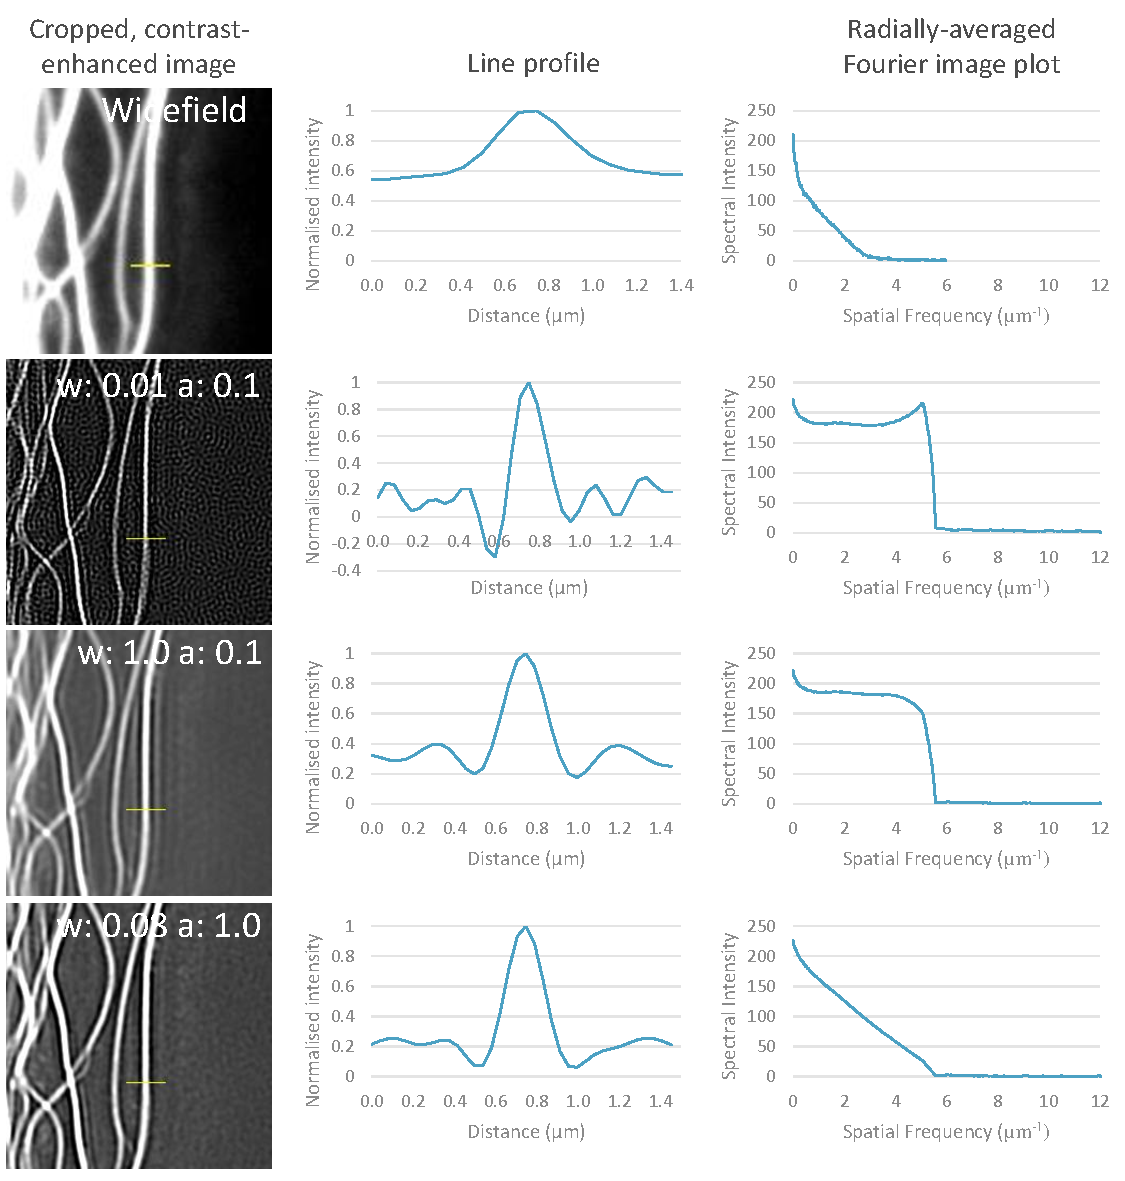
\includegraphics[width=1.0\textwidth]{wiener-parameter}
\caption[LAG SIM: The Wiener parameter and apodisation strength must be chosen to minimise artefacts]{The left column shows crops from a SIM reconstruction with various values of Wiener parameter ($w$) and apodisation strength ($a$), and a widefield image for comparison. Note that image contrast has been greatly enhanced to make the noise pattern visible. The middle column shows the line profile through a tubule, showing the noise pattern with a low Wiener parameter, ringing with a high Wiener parameter, and suppression of noise and ringing using apodisation. The right hand column shows the radially averaged Fourier transform plot of each image; note the local peak when a low Wiener filter is used, which boosts noise at this frequency causing the unconventional noise pattern.}
% Really need to add a, b, c, etc to this, I think.
\label{fig:wiener-parameter}
\end{figure}

Aggressive noise removal, using high values for the Wiener parameter, can cause ringing in the reconstructed images, clearly visible as side-lobes around the $w=1.0$ reconstruction in Figure~\ref{fig:wiener-parameter}~\cite{righolt2013image}.
To reduce ringing artefacts, the reconstructed image is passed through an apodisation filter.

Apodisation applies a smooth low-pass filter, gradually reducing power in higher spatial frequencies avoiding a sharp cutoff.
The radius of the apodising filter in Fourier space is controlled by the `apodisation cutoff' parameter, where a value of 1 corresponds to the cutoff spatial frequency of the objective lens based on its numerical aperture and the emission wavelength of the image.
The shape of the apodisation filter is controlled by the `apodisation strength' parameter, where a value of 0 gives a tophat filter, $\frac{1}{\sqrt{2}}$ a triangular filter, and larger values further reduce the full-width half maximum.

The apodisation cutoff should be set to the same value as the resolution enhancement given in Table~\ref{tab:resolution}, with a maximum value of 2.04 for full SIM resolution enhancement.
Smaller cutoff values reduce the radius of the reconstruction in Fourier space, directly reducing resolution; a value of 1 corresponds to widefield resolution.
The apodisation strength should be as small as possible whilst still removing ringing artefacts for maximum contrast of high-frequency features.

\subsection{Richardson-Lucy filtering introduces less artefacts when optical sectioning is not required} \label{sec:RL-filter}
An alternative filtering scheme for noise removal is Richardson-Lucy deconvolution~\cite{perez2016optimal}.
The Richardson-Lucy filtering scheme has several advantages over Wiener filtering: it guarantees non-negative pixel values, removing the need for an apodisation step; it does not cause ringing in the reconstructed image; and it only requires one parameter to control the level of noise removal, simplifying the reconstruction process for the LAG SIM user~\cite{perez2016optimal, eichstadt2013comparison}.

\begin{figure}[p]
\centering
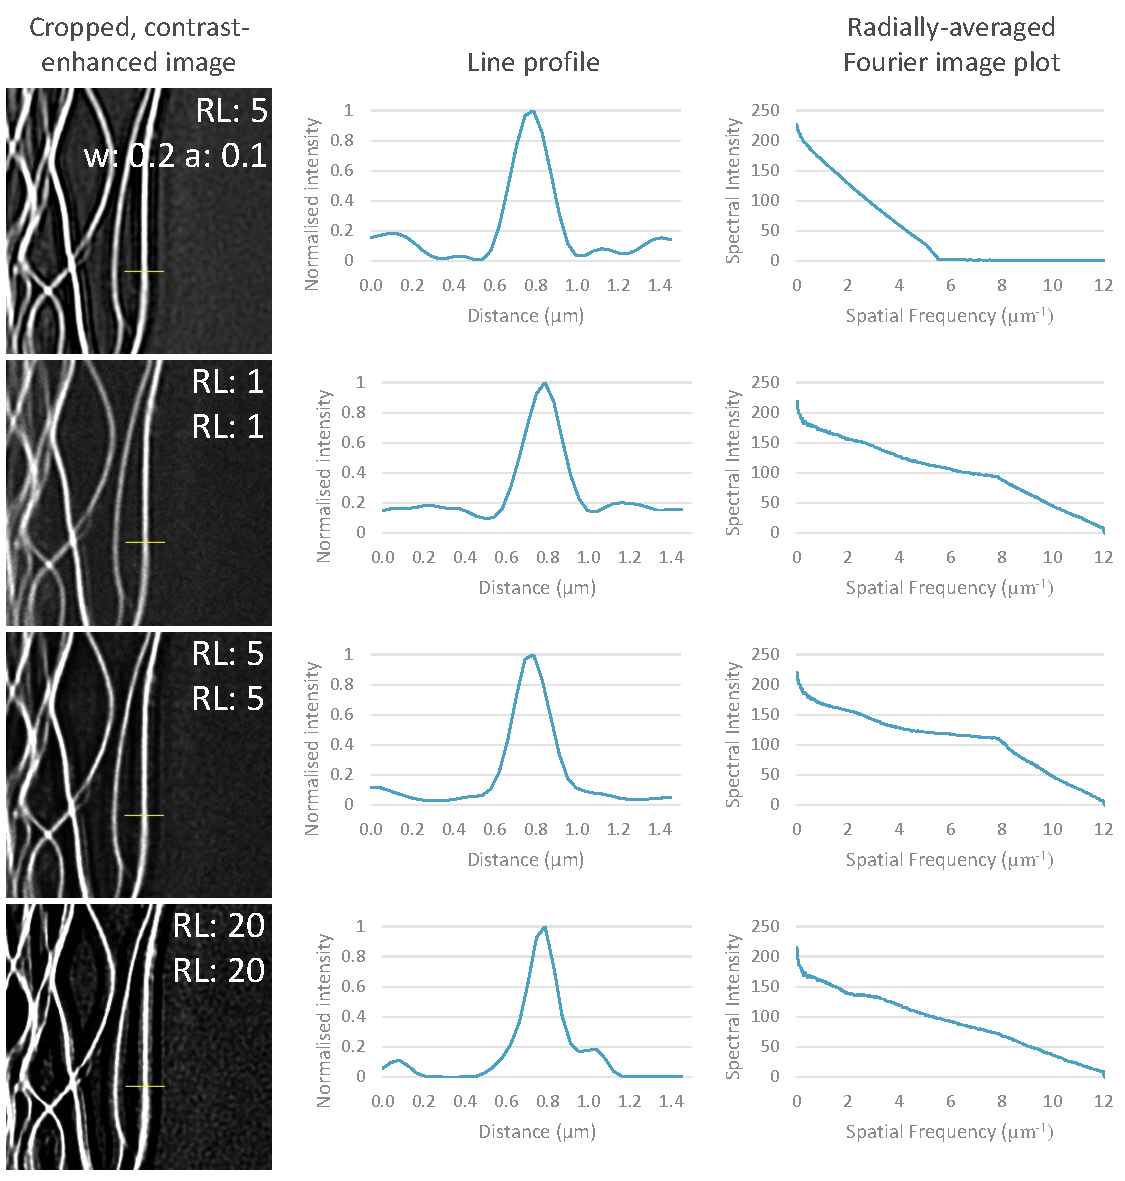
\includegraphics[width=1.0\textwidth]{rl-filtering-figure}
\caption[LAG SIM: Richardson-Lucy filtering can further reduce SIM reconstruction artefacts]{Richardson-Lucy deconvolution on the raw data reduces noise, leading to fewer artefacts in the Weiner-filter reconstruction. Furthermore using Richardson-Lucy filtering for reconstruction produces a more conventionally shaped OTF than Wiener filtering, which further reduces the number of reconstruction artefacts.}
\label{fig:rl-filtering}
\end{figure}

Richardson-Lucy deconvolution is an iterative process, where each iteration of the algorithm converges on the maximum likelihood solution of an image corrupted with Poisson noise~\cite{richardson1972bayesian, lucy1974iterative}.
The number of iterations is set by the user in LAG SIM.
More iterations result in a narrower point spread function, and thus higher perceived resolution; but can also lead to noise amplification, causing speckle patterns to appear in the reconstructed image.

Row 1 in Figure~\ref{fig:rl-filtering} shows Richardson-Lucy deconvolution applied to the input images before conventional SIM reconstruction through the Wiener filter.
This pre-filtering is effective at removing hexagonal SIM artefacts, since less noise is shifted and boosted in Fourier space.

Richardson-Lucy filtering can also be used on the final reconstructed image in place of Wiener filtering.
Figure~\ref{fig:rl-filtering} shows that as the number of iterations is increased from 1 to 20, bumps in Fourier space caused by SIM reconstruction are smoothed out.
This narrows the width of the reconstructed line, but can also lead to artificial amplification when the number of iterations is too high.

Richardson-Lucy input filtering can be used in combination with either the Wiener filter or with more Richardson-Lucy filtering on the reconstructed image.
Therefore there are in total 4 filtering schemes offered by LAG SIM: Wiener-output; RL-output; RL-input, Wiener-output; and RL-input, RL-output.

\subsection{OTF attenuation facilitates resolution-enhanced SIM with optical sectioning}\label{sec:LAGSIM-OTF-attenuation}
In conventional widefield microscopy, light from areas above and below the focal plane are captured by the lens, causing out-of-focus light and reducing the axial resolving contrast of the microscope.
When observing the 3D widefield OTF, shown in red in Figure~\ref{fig:oholleran-otf}, it is clear why this is the case.
The OTF has no support in the axial direction $z$ at low frequencies, which is known as the `missing cone' problem~\cite{sheppard1992significance}.

In the Laser Analytics Group's SIM setup, the illumination pattern is only projected onto the sample plane; therefore out-of-focus light does not show the SIM pattern.
Intuitively, one would think this out-of-focus light can be removed by computationally rejecting any part of the image that does not have the SIM pattern, and only showing the in-focus parts of the image with SIM pattern on them.
O'Holleran and Shaw show that this is achieved practically by attenuating certain parts of the OTF during reconstruction~\cite{oholleran2014optimized}.

If the center part of the OTF is computationally removed, out-of-focus light will be removed from the reconstructed image.
In conventional widefield microscopy, this would have the side-effect of also removing low-frequency information from the image.
In structured illumination microscopy, however, this information can be recovered from shifted components in Fourier space.

\begin{figure}[htbp!]
\centering
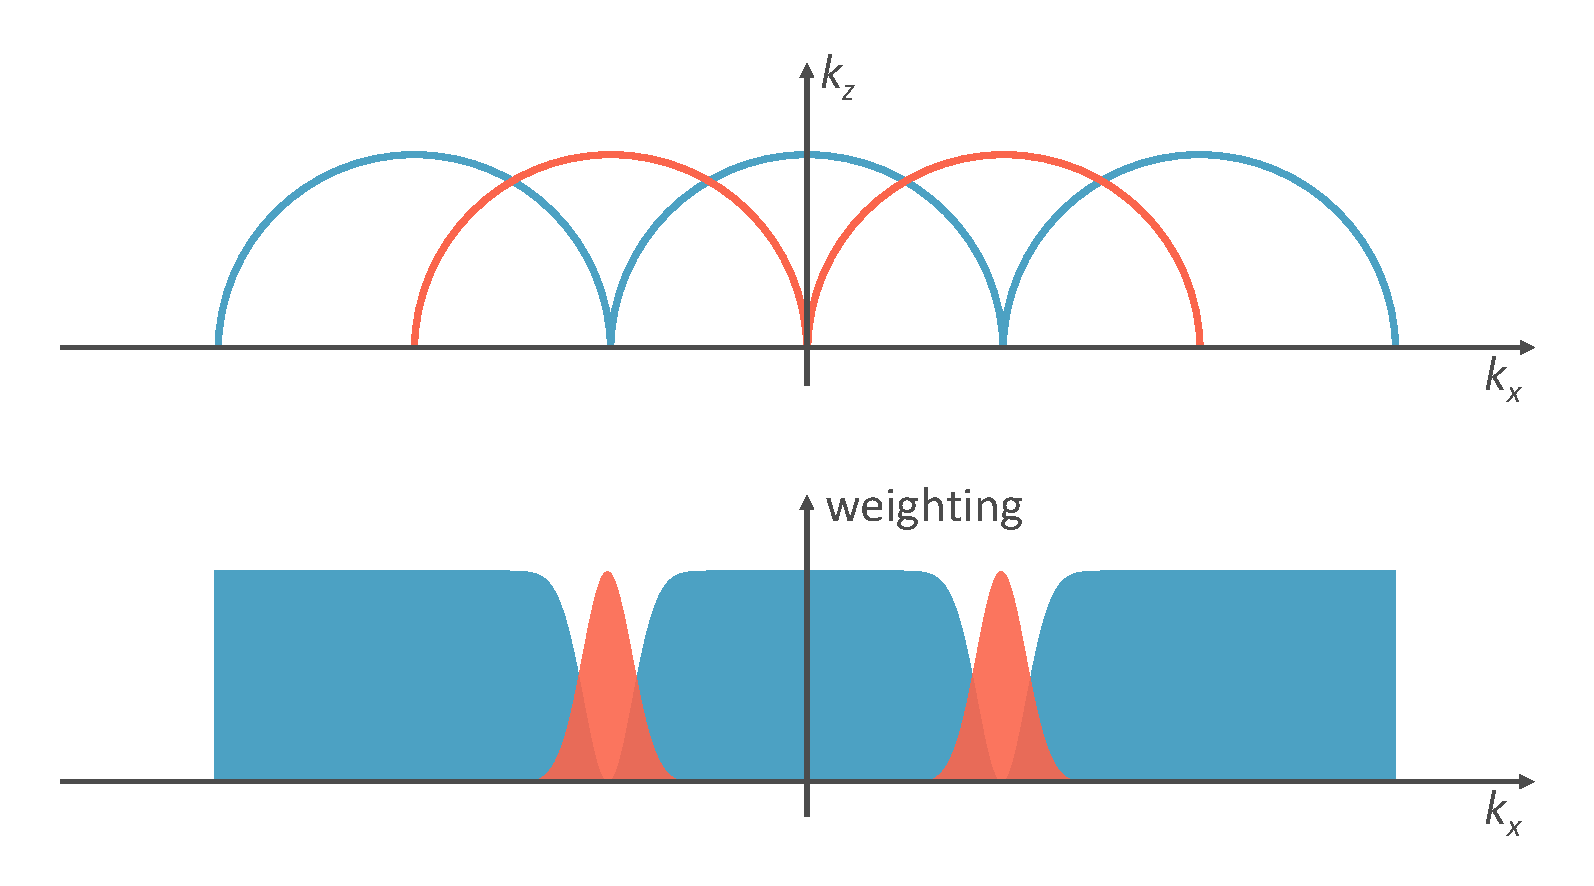
\includegraphics[width=1.0\textwidth]{oholleran-otf-attenuation}
\caption[LAG SIM: OTF attenuation as part of the SIM reconstruction process removes out-of-focus light]{A widefield OTF, shown in red, does not have axial support at low lateral frequencies, leading to out-of-focus light in widefield images. Applying the red weighting as a Fourier-space filter removes this out-of-focus light; however in conventional epifluorescent microscopy, this would also remove low-frequency spatial information. The Fourier-space shifting inherent to SIM reconstruction recovers the attenuated information, as shown by the blue line, providing support at low lateral frequencies. When the shifted components are filtered by the blue weighting, which removes their own out-of-focus light, an optically-sectioned resolution-enhanced image can be reconstructed.  Adapted from~\cite{oholleran2014optimized}. }
\label{fig:oholleran-otf}
\end{figure}

Figure~\ref{fig:oholleran-otf} shows which parts of the OTF should be attenuated to achieve optical sectioning with no loss of resolution.
The optical sectioning is controlled by a Gaussian notch in the first-order passbands, shown in blue, and a complementary Gaussian in the zero-order passband, shown in red.
The width and depth of this passband is controlled in LAG SIM with the parameters `Attenuation FWHM' and `Attenuation strength' respectively, which control how much out-of-focus light is rejected from the image.

\begin{figure}[tbp]
\vspace{-6pt} \centering
\begin{subfigure}[b]{0.49\textwidth}
	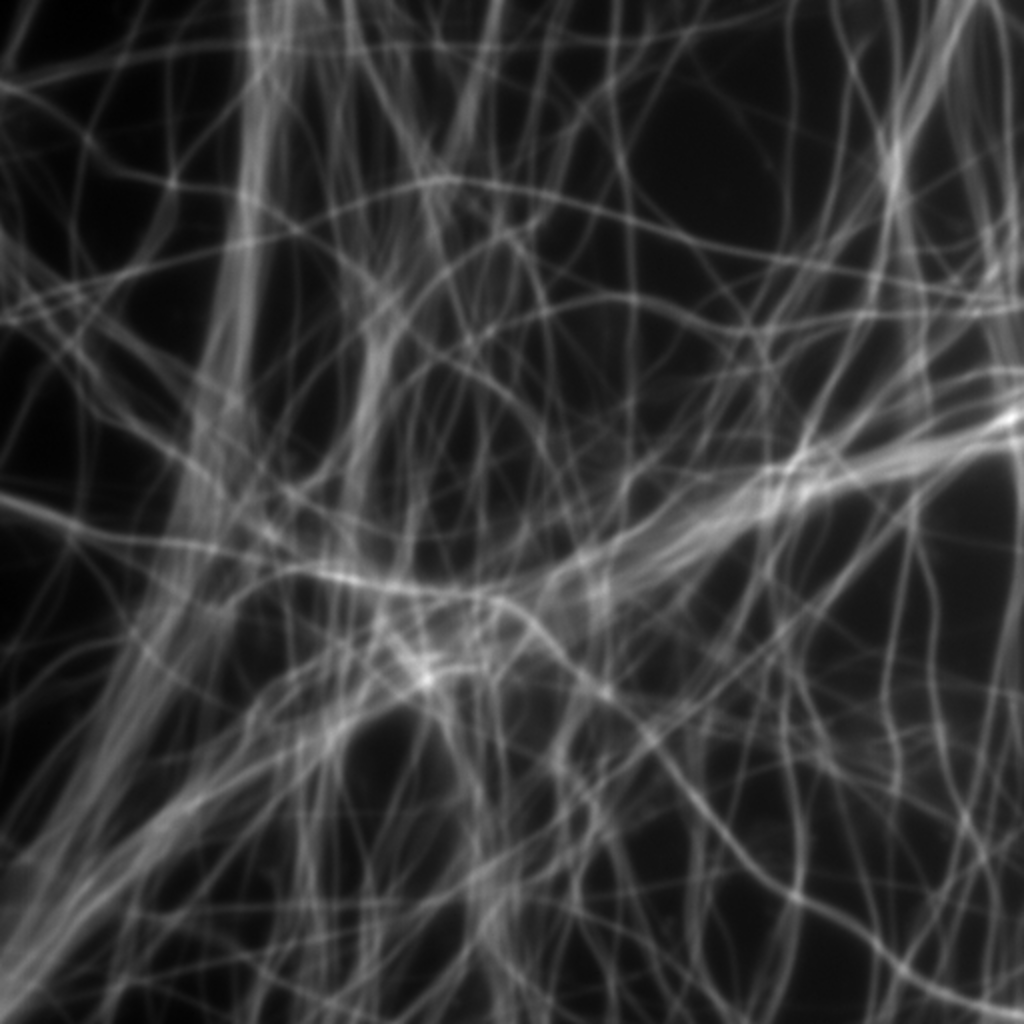
\includegraphics[width=\textwidth]{os-wide-s}
	\caption{}\label{fig:os-wide-s}
\end{subfigure}
~
\begin{subfigure}[b]{0.49\textwidth}
	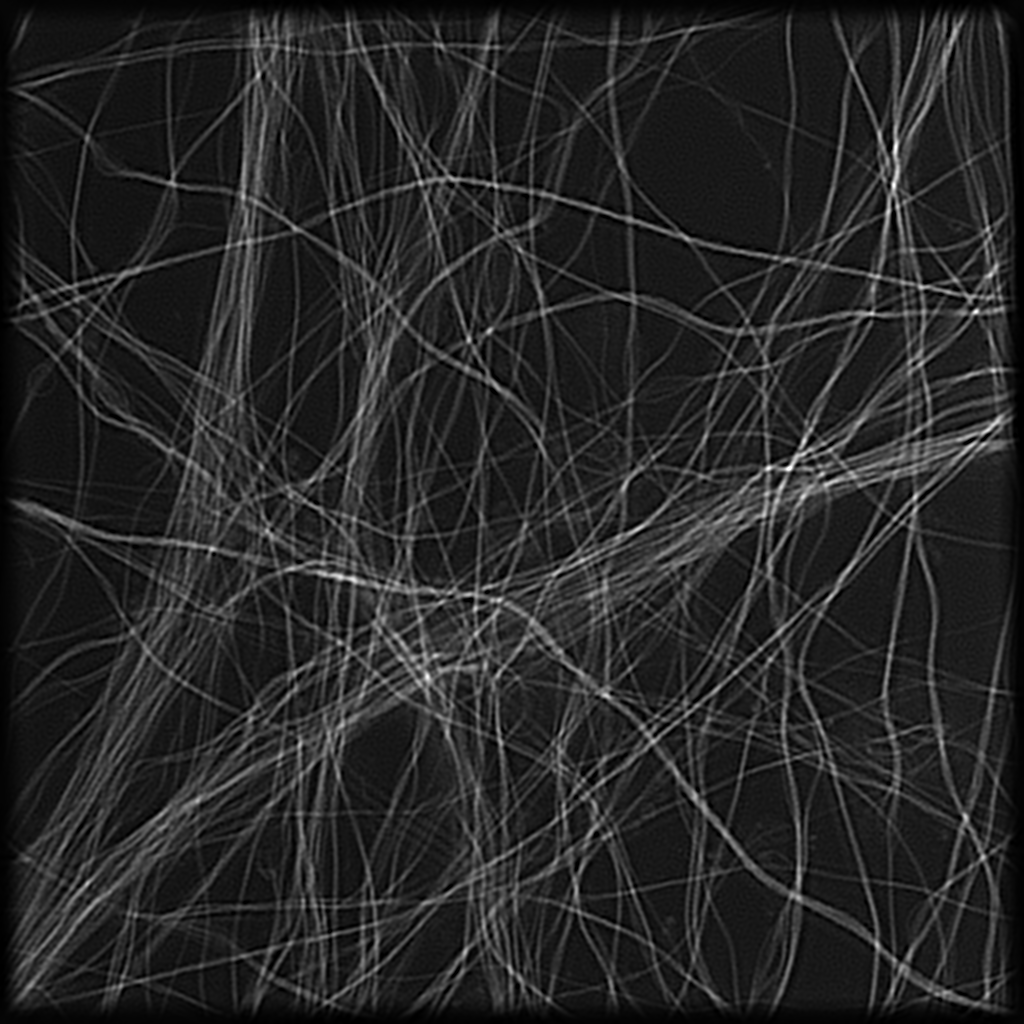
\includegraphics[width=\textwidth]{os-w-s}
	\caption{}\label{fig:os-w-s}
\end{subfigure}
~\newline
\begin{subfigure}[b]{0.49\textwidth}
	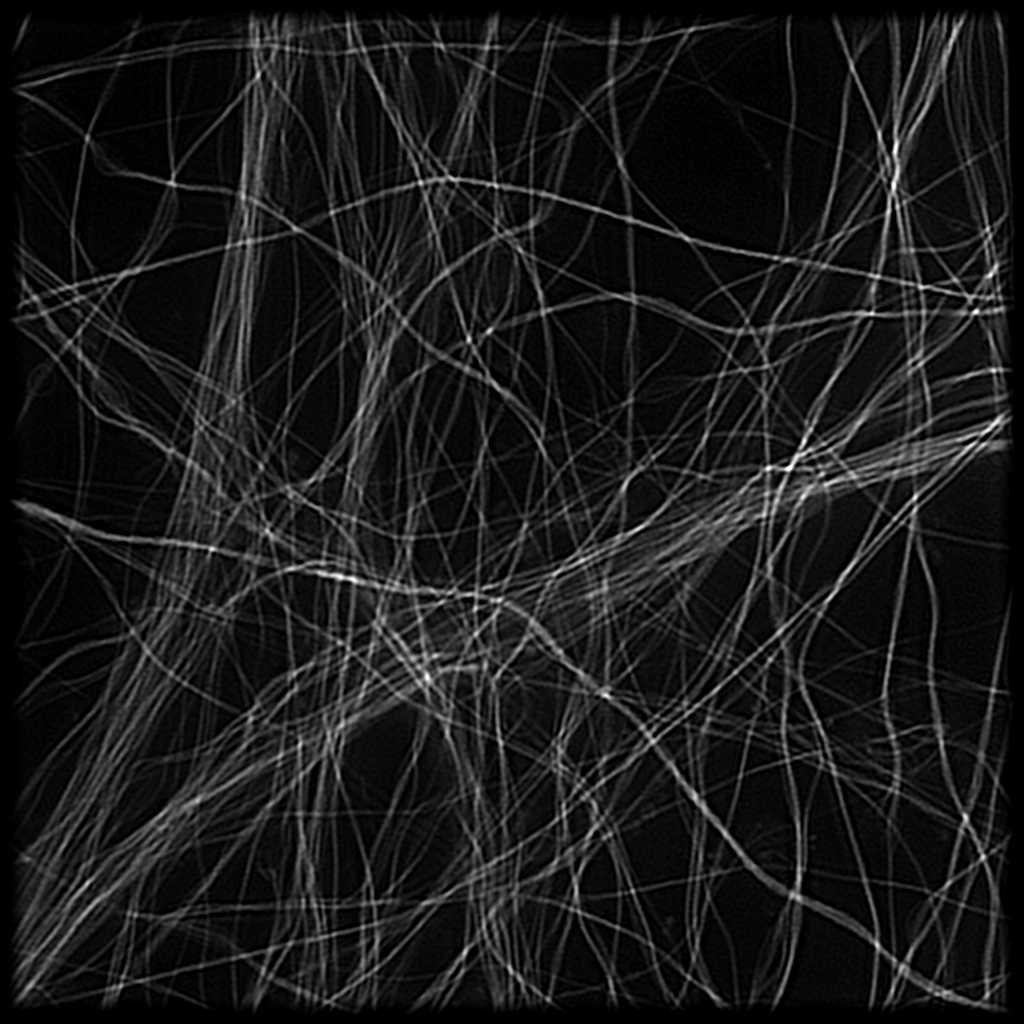
\includegraphics[width=\textwidth]{os-otf-s}
	\caption{}\label{fig:os-otf-s}
\end{subfigure}
~
\begin{subfigure}[b]{0.49\textwidth}
	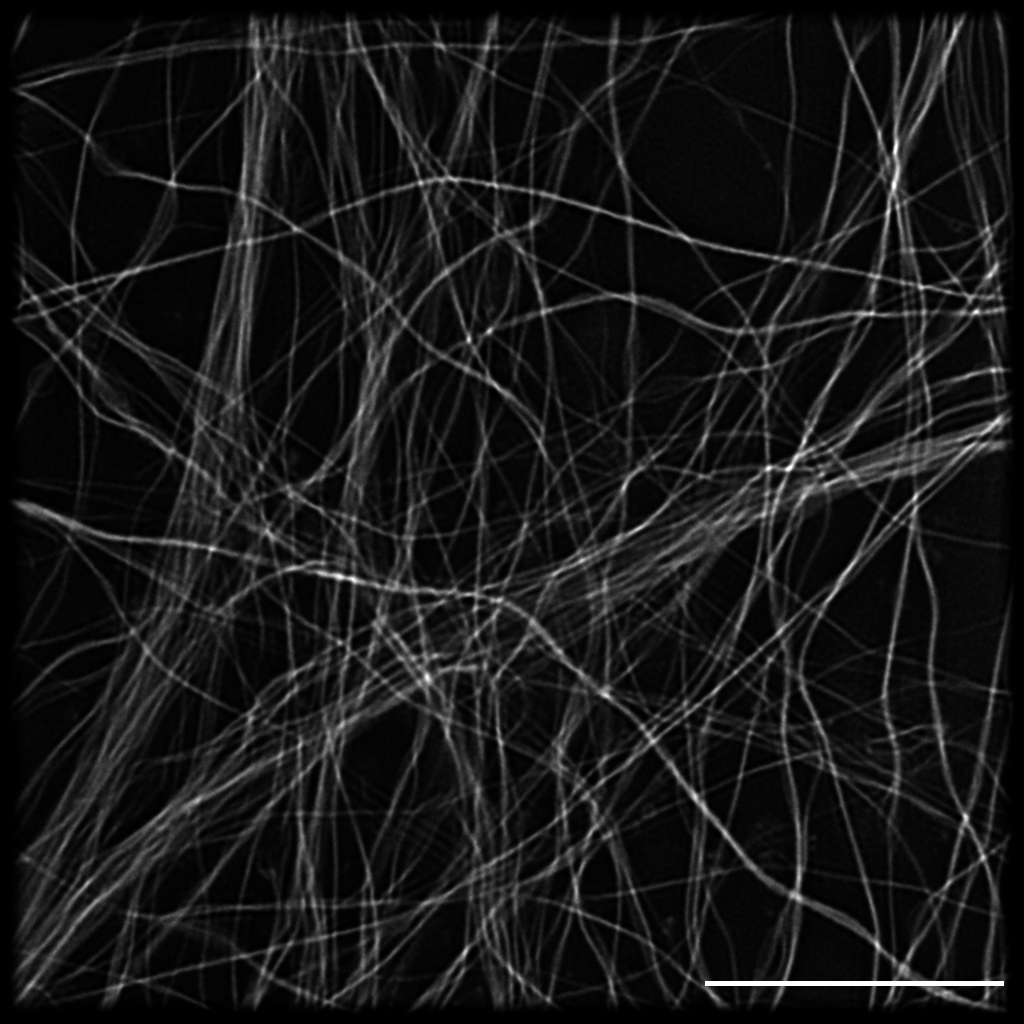
\includegraphics[width=\textwidth]{os-rl-s}
	\caption{}\label{fig:os-rl-s}
\end{subfigure}
\caption[LAG SIM: Optical sectioning through OTF attenuation removes out-of-focus light]{The images show a slice from a z-stack of microtubules. (a) Shows a widefield image, where out-of-focus light reduces the contrast of tubules in the focal plane. (b) shows a SIM reconstruction Wiener reconstruction, where the out-of-focus light causes ringing artefacts. (c) shows a SIM Wiener reconstruction with OTF attenuation applied, with a attenuation FWHM of 1.2 and an attenuation strength of 0.995. (d) shows a SIM reconstruction using the Richardson-Lucy filter, which removes out of light through deconvolution. Samples were prepared and labelled by Miranda Robbins. Scalebar is \SI{10}{\micro\metre}.}
\label{fig:OS-slice-examples}
\end{figure}

\begin{figure}[tbp]
\vspace{-6pt} \centering
\begin{subfigure}[b]{0.49\textwidth}
	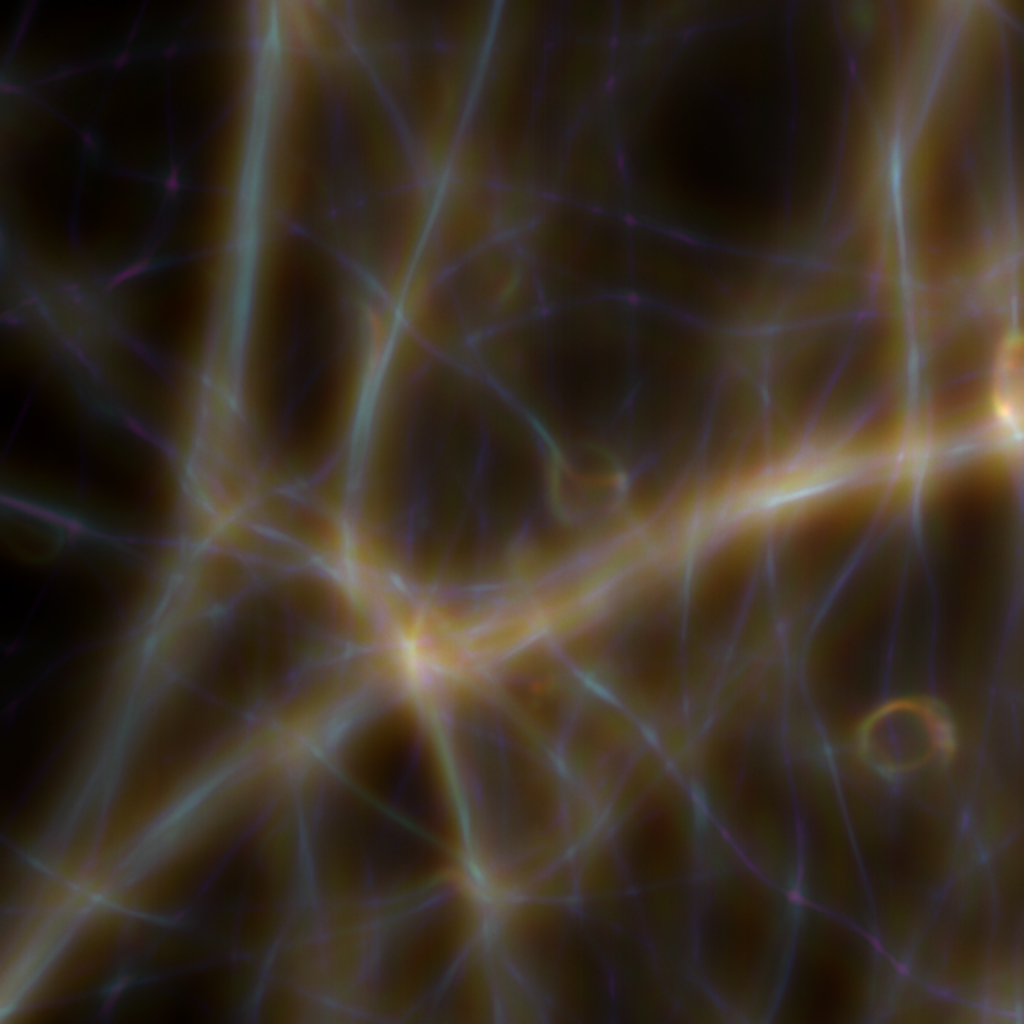
\includegraphics[width=\textwidth]{os-wide-c}
	\caption{}\label{fig:os-wide-c}
\end{subfigure}
~
\begin{subfigure}[b]{0.49\textwidth}
	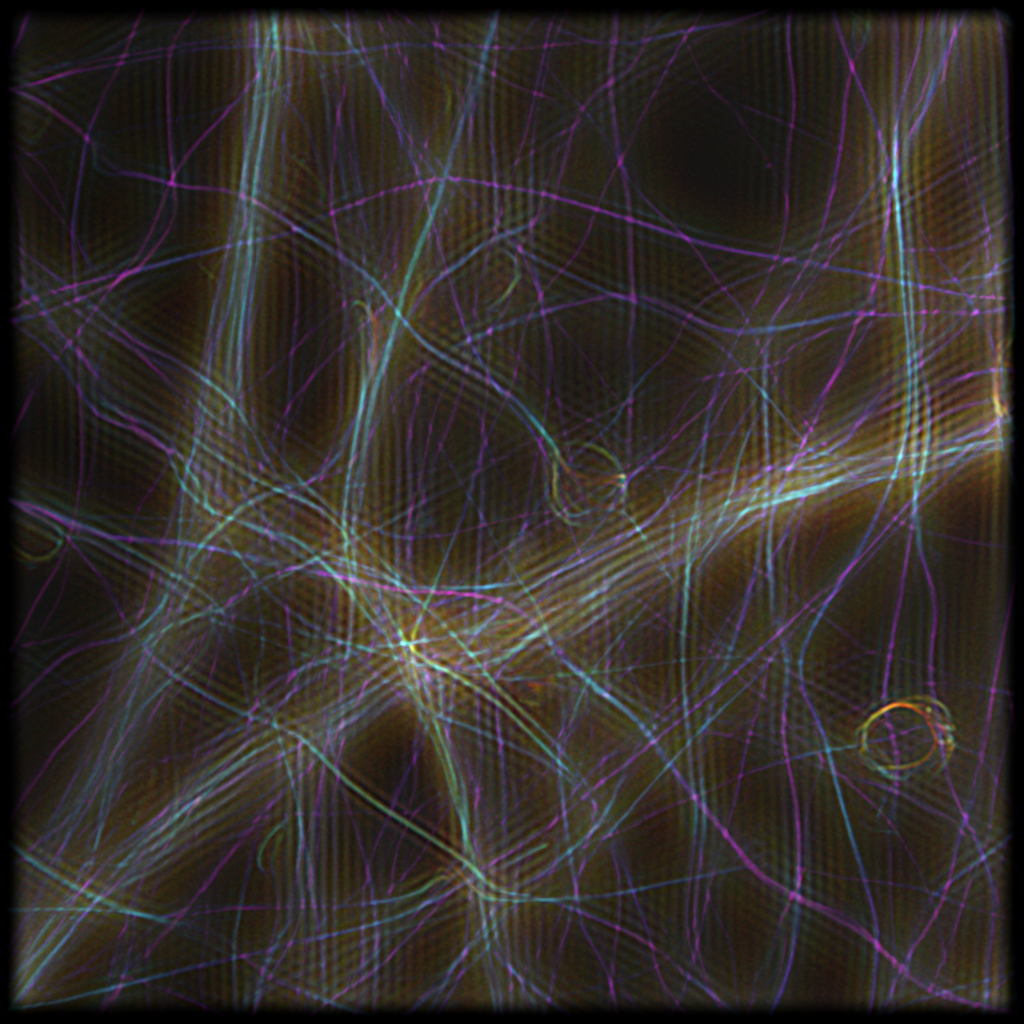
\includegraphics[width=\textwidth]{os-w-c}
	\caption{}\label{fig:os-w-c}
\end{subfigure}
~\newline
\begin{subfigure}[b]{0.49\textwidth}
	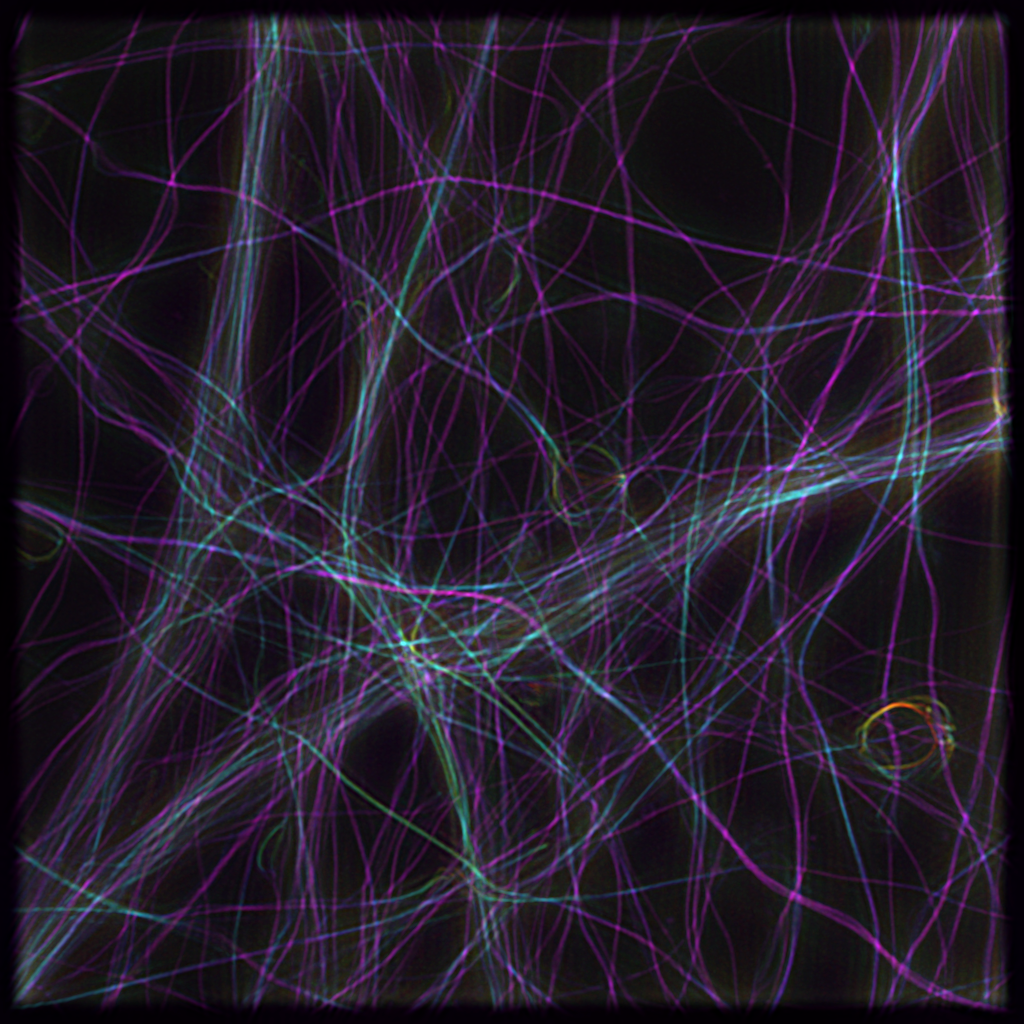
\includegraphics[width=\textwidth]{os-otf-c}
	\caption{}\label{fig:os-otf-c}
\end{subfigure}
~
\begin{subfigure}[b]{0.49\textwidth}
	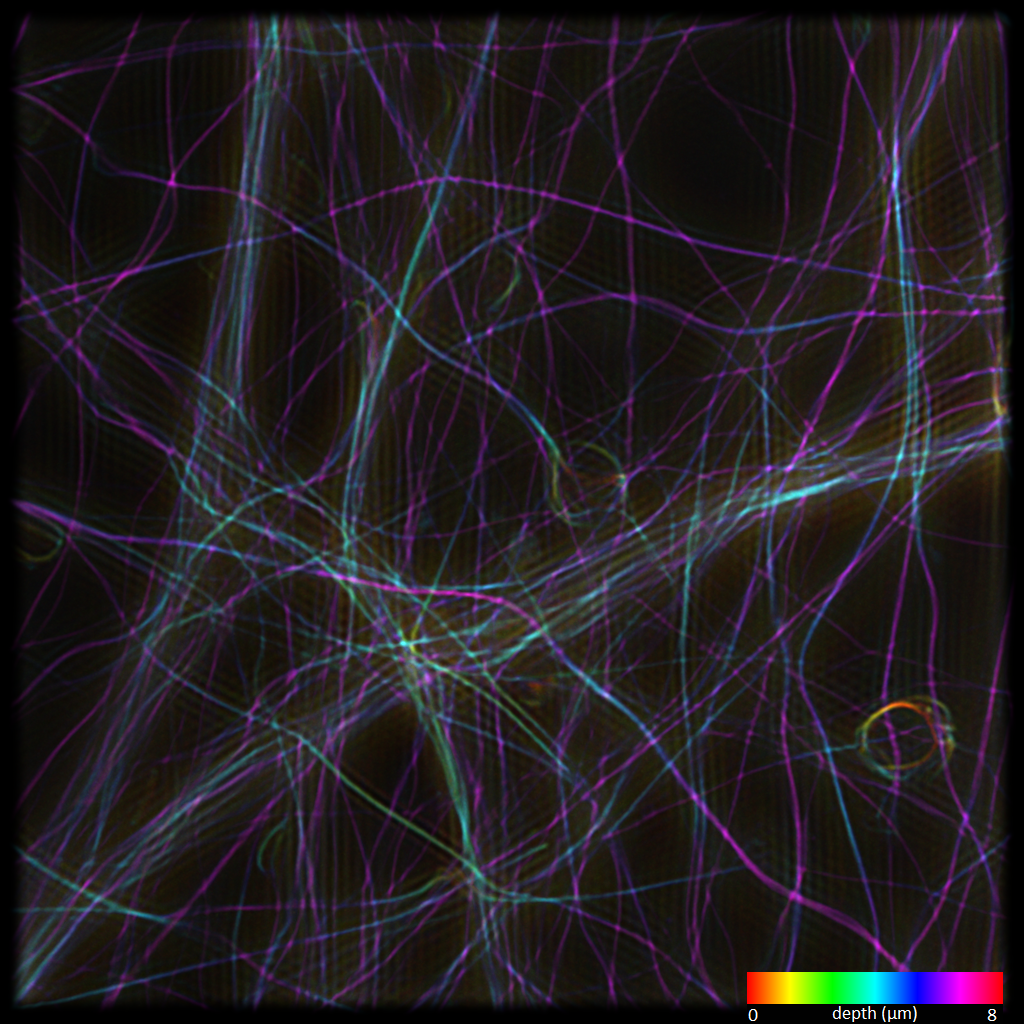
\includegraphics[width=\textwidth]{os-rl-c}
	\caption{}\label{fig:os-rl-c}
\end{subfigure}
\caption[LAG SIM: Removing out-of-focus reveals 3D structure]{The figure shows a 3D stack of microtubules coloured by depth. The reconstruction methods shown are the same as for Figure~\ref{fig:OS-slice-examples}: (a) is a widefield image; (b) a SIM reconstruction with Wiener filtering; (c) a SIM reconstruction with OTF attenuation applied; and (d) a SIM reconstruction using the Richardson-Lucy filter. Samples were prepared and labelled by Miranda Robbins. Colorbar represents relative depth from \SI{0}{\micro\metre} to \SI{8}{\micro\metre}.}
\label{fig:OS-colored-examples}
\end{figure}


Out-of-focus light makes creating 3D reconstructions impossible. 
The widefield images of microtubules in Figures~\ref{fig:os-wide-s} and \ref{fig:os-wide-c} show that out-of-focus light reduces the contrast of tubules in the focal plane, so that its position in the $z$-direction cannot be determined. Figures~\ref{fig:os-w-s} and \ref{fig:os-w-c} show a standard SIM reconstruction using a Wiener filter as described in Section~\ref{sec:wiener-recon} - the out of focus information has caused artefacts to appear in the image, clearly visible as ringing in the z-projection image. By using OTF attenuation, the out-of-focus light and therefore the ringing artefacts can be removed, as shown in Figures~\ref{fig:os-otf-s} and \ref{fig:os-otf-c}. 

Note that OTF attenuation cannot be used with the Richardson-Lucy output filter.
However, since it is a deconvolution algorithm, reconstruction by the Richardson-Lucy filter as described in Section~\ref{sec:RL-filter} removes out-of-focus light, seen in Figures~\ref{fig:os-rl-s} and \ref{fig:os-rl-c}.
The disadvantage compared to using OTF attenuation, however, is the lack of control over how much out-of-focus light to reject, since the only input parameter to the Richardson-Lucy filter is the number of iterations.
Therefore if optical sectioning is required, it is recommended to use the "RL-in, Wiener-out" filtering scheme with the OTF attenuation checkbox ticked.

Using optical sectioning to remove the out-of-focus light allows 3D reconstructions of the sample to be created. 
This can reveal information otherwise unobservable, such as whether a particle is located on the inside or outside of a cell membrane~\cite{teplensky2017temperature}.


\section{Results and Discussion} \label{sec:sim-showcase}
LAG SIM has been designed to be a versatile and user-friendly microscope, providing high-speed multicolour imaging surpassing the diffraction limit with optical sectioning provided computationally or with TIRF.
With a number of useful automations, LAG SIM can be used to create timelapse videos, 3D reconstructions, large mosaic images, and for unsupervised imaging of multiple cells at different locations around the coverslip.
As a result, the microscope has found applications in a wide variety of biological investigations.

Two such investigations are discussed in detail in Chapters~\ref{chap:MOF} and \ref{chap:ER}.
This section, however, presents a brief overview of a diverse selection of experiments demonstrating a wide range of LAG SIM's capabilities.
Acquisition and reconstruction methods are provided as a resource for researchers interested in conducting similar experiments with the microscope.

\subsection{Multicolour beads for chromatic alignment}
For multicolour SIM experiments, small chromatic offsets between colour channels, shown in Figure~\ref{fig:recon-beads-unaligned}, require that image registration is performed.
A slide of multicolour sub-diffraction beads can be used for measuring and correcting chromatic offset, because the well-defined points of light have the same spatial distribution in each colour channel.

For effective registration, the correct density of beads is required, and the beads should be well separated.
A dense region of beads will form a homogeneous layer across the microscope slide, without well-defined bead coordinates, so cannot be used for registration.
Conversely if the density of beads is too low then too few beads per field-of-view reduces the accuracy of registration.

A microscope slide or Labtek\texttrademark\ well with an appropriate density of beads can be prepared as follows:
\begin{enumerate}
	\item Sonicate \SI{0.1}{\micro\metre} beads for \SI{10}{\minute}
	\item Dilute beads 1:10 in distilled water, producing a \SI{1.8e10}{particles\per\milli\litre} suspension density
	\item Dispense \SI{20}{\micro\litre} of the diluted beads onto a coverglass, or \SI{50}{\micro\litre} into an 8-well Labtek
	\item Wait for the solution to dry, about \SI{2}{\hour}
	\item Add mounting medium: immersion oil for use with the 100$\times$ oil lens, or water for use with the 60$\times$ water lens.
	\item Mount the coverglass on a glass slide, or replace the lid on the Labtek\texttrademark\ and seal with Parafilm\texttrademark\  to prevent spillages
\end{enumerate}

Following this protocol produces a bead sample with about 100 particles per field-of-view.
The sonication step means that beads are well spread out, so that individual beads can be accurately localised.

\begin{figure}[p]
\centering
\begin{subfigure}[b]{0.49\textwidth}
	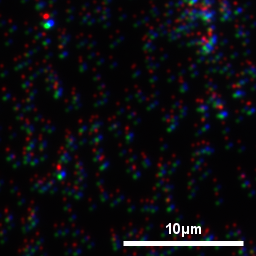
\includegraphics[width=\textwidth]{recon-beads-unaligned}
	\caption{}\label{fig:recon-beads-unaligned}
\end{subfigure}
\hfill
\begin{subfigure}[b]{0.49\textwidth}
	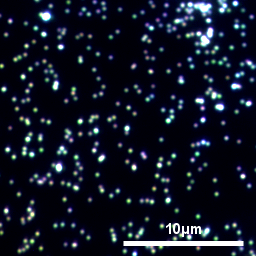
\includegraphics[width=\textwidth]{recon-beads-registered}
	\caption{}\label{fig:recon-beads-registered}
\end{subfigure}
\caption[LAG SIM: Multicolour alignment beads are used for correcting chromatic offset]{A small chromatic offset between the three SIM colour channels can be seen in (a). When the offset is corrected, as in (b), the beads appear white; the offset parameters can then be used to correct other multicolour images captured during the same imaging session.  }
\label{fig:recon-beads}
\end{figure}
\afterpage{\clearpage}

Before capturing images, the bead sample can also be used for minimising spherical aberrations introduced by temperature changes and refractive index mismatches.
When the bead sample is viewed on the microscope, adjusting the correction collar on the objective lens will change the shape of each bead's point-spread function.
For minimal aberrations, the point-spread function should be symmetrical when defocussing above and below the bead layer.

To measure chromatic offset, a multicolour SIM acquisition should be captured in the same colour channels as the subsequent biological experiment.
The single layer of beads will not have contribution from out-of-focus light, and should also have a high signal-to-noise ratio.
Therefore the SIM reconstruction process does not require OTF attenuation for optical sectioning, so the Richardson-Lucy filter is recommended on the output stage of the reconstruction process.
Section~\ref{sec:RL-filter} shows that 5 iterations of filtering reduce noise without introducing artefacts.
The suggested parameters to enter into the LAG SIM Fiji plugin are summarised as follows: \newline
\begin{tabular}{p{0.5\textwidth}}
\begin{labelling}[margin=OTF attenuation]
	\item[Filter] RL out
	\item[RL steps] 5
	\item[OTF attenuation] false
\end{labelling}
\end{tabular}

After reconstruction, there will be some chromatic offset between each channel, as shown in Figure~\ref{fig:recon-beads-unaligned}.
After registration and correction, Figure~\ref{fig:recon-beads-registered} shows that a red-green-blue (RGB) colour map will produce white beads.
These same registration parameters can then be used for other multicolour experiments in the same imaging session.


\subsection{Resolution-enhanced optical sectioning of HeLa cells shows MOF colocalised with endosomes} \label{sec:showcase-MOF}
A frequent biological application of microscopy is imaging cultured cells under different treatments or with different genetic modifications~\cite{white1987evaluation, specht2017critical, wang2017analysis}.

Collaborators in the department had been developing a drug delivery system based on metal organic frameworks (MOFs), and wanted to observe the treatment to ensure MOFs were taken up by cells for delivery of their payload.
In this particular application, which Chapter~\ref{chap:MOF} describes in much greater detail, calcein was loaded into the porous structure of crystalline MOFs as a model drug.
This MOF treatment was incubated with HeLa cells for \SI{24}{\hour}, and uptake over time was captured with microscopy.

Widefield images had shown MOF located at the cell membrane; however widefield's inherent lack of optical sectioning meant that conclusions could not be drawn from these images about whether the MOF was inside or outside the cell~\cite{orellana2015amorphous}.

One microscopy technique often used to provide optical sectioning is confocal imaging; this was unsuitable for this experiment for several reasons.
Firstly, confocal microscopy has a resolution limit of \SI{200}{\nano\metre}.
The MOF used in this experiment forms crystalline structures on the order of \SI{100}{\nano\metre}, so a higher resolution was required to accurately capture their location.
Secondly, acquiring a z-stack of confocal images to produce a 3D model of the cell, which is necessary for determining if the MOF is within the cell membrane, is a slow process, with a 3-channel acquisition taking at least \SI{5}{\minute} per cell~\cite{jonkman2015any}.
Since the cells could only survive on the microscope stage for \SI{2}{\hour}, this limited the number of cells which could be captured per imaging session.

The LAG SIM was able to address both these issues.
It provides optical sectioning with resolution enhancement, resolving the MOFs and accurately determining their location.
It is also able to capture images faster, requiring just 9 images per plane, rather than point-scanning which takes longer to capture the same amount of florescence emission light~\cite{jonkman2015any}.

To observe uptake using the laser lines available on the LAG SIM, the following labelling scheme was designed:
calcein, which naturally is fluorescent when illuminated with \SI{488}{\nano\metre} excitation light, was used as the model drug loaded into the MOFs;
endosomes were labelled with CellLight Early Endosomes-RFP BacMam 2.0; and the nucleus was labelled with HCS NuclearMask™ Deep Red Stain to visualise the cell.
The LAG SIM's laser lines, \SI{488}{\nano\metre}, \SI{561}{\nano\metre}, and \SI{640}{\nano\metre}, could then be used to excite fluorescence for the MOFs, endosomes, and nucleus respectively.

Since fast dynamics were not observed, a \SI{200}{\milli\second} exposure time was used per raw frame.
This relatively long exposure time ensured high signal-to-noise ratio.
Similarly, to minimise cross-talk between imaging channels the Optosplit was not employed and filtering was performed by filters in the filter wheel.

To determine whether MOF had entered the cell or was simply sitting on the cell membrane, it was necessary to view the cells in 3D.
The 60$\times$ water lens was selected, and operated in optical sectioning SIM mode.
Images were captured at every \SI{200}{\nano\metre} in the axial direction, to build up a Nyquist-limited z-stack.

To provide optical sectioning the z-stack was reconstructed in the LAG SIM Fiji plugin with OTF attenuation.
The full-width half-maximum and depth of the attenuation Gaussian, defined in Section~\ref{sec:LAGSIM-OTF-attenuation}, were set to 1.2 and 0.995 respectively.
These values generally work well to remove out-of-focus light from reconstructed images without introducing artefacts.

Since OTF attenuation was applied, the Richardson-Lucy filter could not be used on the output stage of the reconstruction; however 5 Richardson-Lucy iterations were applied to the input data to prevent noise-boosting in the reconstruction process, as described in Section~\ref{sec:RL-filter}.
The Wiener parameter was set to the relatively low value of 0.03 by virtue of the high signal-to-noise ratio of the raw data.
The apodisation cutoff was set to 1.6 for the \SI{488}{\nano\metre} and \SI{640}{\nano\metre} channels, and 1.67 for the \SI{561}{\nano\metre} channel, since this is the factor of resolution enhancement provided in 60X optical-sectioning SIM, listed in Table~\ref{tab:resolution}.
Finally the attenuation strength was set to 0.8, to ensure that the OTF of the reconstructed image has the same shape as a conventional OTF, which prevents ringing artefacts.

The parameters required for the LAG SIM Fiji plugin are summarised as follows:
\newline
\begin{tabular}{p{0.5\textwidth}p{0.5\textwidth}}
\begin{labelling}[margin={Attenuation strength}]
	\item[Filter] RL in, Wiener out
	\item[Wiener parameter] 0.03
	\item[Apodiation cutoff] 1.6
	\item[Apodiation strength] 0.8
\end{labelling} &
\begin{labelling}[margin={Attenuation strength}]
	\item[RL steps] 5
	\item[OTF attenuation] true
	\item[Attenuation FWHM] 1.2
	\item[Attenuation strength] 0.995
\end{labelling}
\end{tabular}

\begin{figure}[tbp!]
\centering
\begin{subfigure}[b]{0.7\textwidth}
	\includegraphics[width=\textwidth]{recon-mofcell-2D}
	\caption{}\label{fig:recon-mofcell-2D}
\end{subfigure}

~\newline
\begin{subfigure}[b]{0.7\textwidth}
	\includegraphics[width=\textwidth]{recon-mofcell-3D}
	\caption{}\label{fig:recon-mofcell-3D}
\end{subfigure}
\caption[LAG SIM: 3D SIM reconstruction reveals that MOFs are endocytosed by HeLa cells]{(a) shows a 3-colour SIM reconstruction overlaid on a brightfield image of a cell, with MOF coloured in green, endosomes coloured in magenta and the nucleus coloured in cyan. MOF can be seen located within the cell boundary, and white spots showing colocalisation between green and magenta imply that MOF is taken into cells through an endocytosis pathway. (b) shows another cell with the same colour scheme as a 3D projection, confirming that MOF is truly located within the cell and is not simply sitting on the cell membrane. The 3D data set is available to explore interactively at \mbox{\url{https://fpb.ceb.cam.ac.uk/MOF}}. Cells were prepared for imaging by Michelle Teplensky. Scalebar in (a) is \SI{20}{\micro\metre}. }
\label{fig:recon-mofcell}
\end{figure}
\afterpage{\clearpage}

Figure~\ref{fig:recon-mofcell-2D} shows a 3-colour reconstructed SIM image overlaid on a brightfield image, revealing green MOF particles within the magenta cell boundary.
Furthermore, white spots in the image show colocalisation between green and magenta, implying that MOF has been taken up into the cell through an endocytosis pathway and is localised within endosomes.

To confirm that MOF is truly within the cell boundary and is not sitting on top of the cell requires the 3D reconstructions provided by optical sectioning SIM.
Figure~\ref{fig:recon-mofcell-3D} indeed verifies this.
Whilst some MOF is on the outside of the cell boundary, other fragments of MOF have been endocytosed into the cell.
White areas of the image again verify MOF colocalised with endosomes.

The 3D projection shown in Figure~\ref{fig:recon-mofcell-3D} highlights an issue with presenting 3D data on a static 2D medium.
It is difficult for the reader to understand the orientation and perspective of the data.
For this reason the 3D dataset is also available to explore interactively in a web browser at \url{https://fpb.ceb.cam.ac.uk/MOF}, using the new tool FPBioimage detailed in Chapter~\ref{chap:FPB}.

This drug-delivery experiment highlights the LAG SIM's capability of imaging live cells in 3D by utilising optical sectioning, and also providing resolution enhancement over other techniques.
Details of the experiment are presented in Chapter~\ref{chap:MOF}, including timelapse imaging for observing uptake over a \SI{24}{\hour} period, as well as similar experiments delivering therapeutic drugs to cells with different MOFs.

\subsection[Fast, multicolour imaging of COS-7 cells reveals dynamic colocalisation between ER and lysosomes]{Fast, multicolour imaging of COS-7 cells reveals dynamic\\ colocalisation between ER and lysosomes}
During experiments on the dynamics of endoplasmic reticulum (ER), which are detailed in Chapter~\ref{chap:ER}, we observed a strong interaction between ER and other organelles, including lysosomes and tubulin.
To develop a deeper understanding of these relationships, we required fast, high-resolution imaging of live cells in multiple colour channels simultaneously.

To resolve the shape of lysosomes and the fine network structure of ER requires a microscope capable of resolving structures smaller than \SI{100}{\nano\metre}.
Whilst some super-resolution techniques are able to resolve structures as small as \SI{20}{\nano\metre}, such as STORM and STED, they do not have the imaging speed required to observe fast dynamic events such as ER tubule growth.
LAG SIM is able to provide resolution beyond \SI{100}{\nano\metre}, at 11\,frames per second, suitable for imaging these organelle dynamics.

For high resolution, the 100$\times$ oil lens was chosen, although, because we were looking deeper than \SI{100}{\nano\metre} into the cell, it was not operated in TIRF mode.
To facilitate simultaneous multicolour imaging, the Optosplit was employed.
Cross-talk between colour channels was minimised by labelling just two organelles per experiment, in the \SI{488}{\nano\metre} and \SI{640}{\nano\metre} excitation channels.

\begin{figure}[tbp!]
\centering
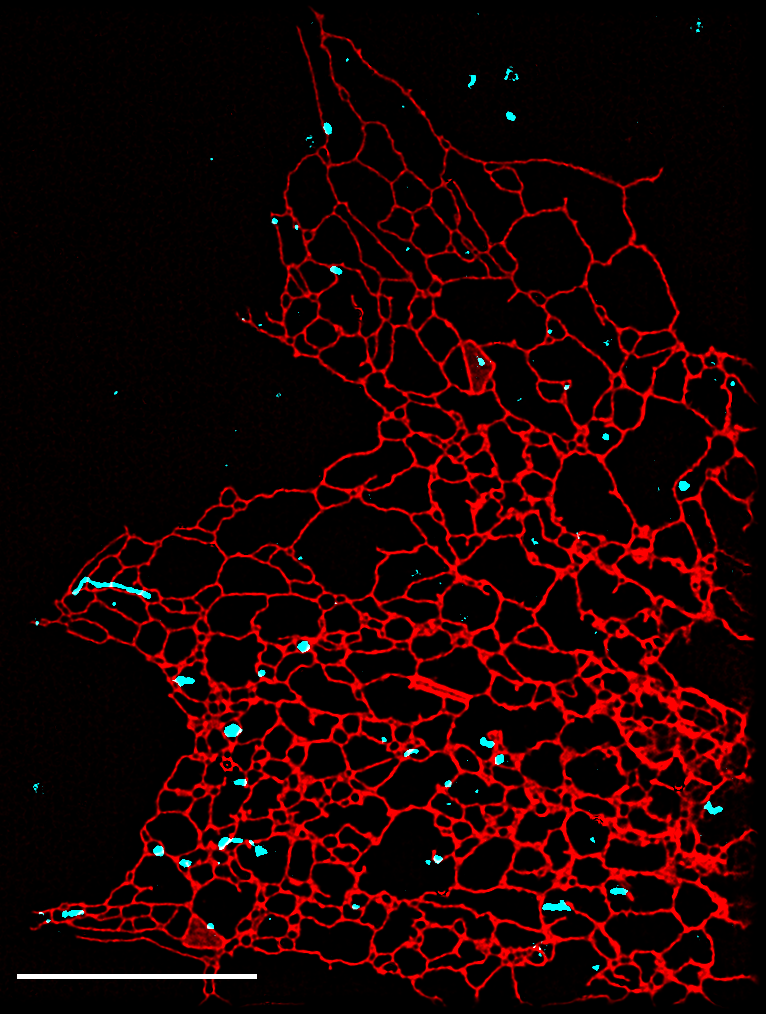
\includegraphics[width=1.0\textwidth]{recon-er-cell}
\caption[LAG SIM: Fast, multicolour imaging of ER in cells reveals co-localisation between lysosomes and ER tubules]{COS-7 cells with ER is coloured in red, and lysosomes are coloured in cyan. Capturing a timelapse utilising the Optosplit and optical sectioning SIM reveals a dynamic colocalisation between lysosomes and ER tubules, where lysosomes appear to pull the ER network to rearrange connections. Cells were cultured and labelled by Meng Lu. Scalebar is \SI{10}{\micro\metre}. }
\label{fig:recon-er-cell}
\end{figure}
\afterpage{\clearpage}

A time-series of SIM images was acquired at a raw exposure time of \SI{10}{\milli\second} per frame, which equates to a reconstructed image rate of \SI{11}{\hertz}.
Since optical sectioniong was not required, the Richardson-Lucy filter was used on both the raw images and for the reconstruction output stage, as described in Section~\ref{sec:RL-filter}.
Richardson-Lucy filtering was performed with 5 iterations, which Figure~\ref{fig:rl-filtering} shows gives a good balance of noise suppression without noise amplification, leading to artefact-free images.
The parameters required for the LAG SIM Fiji plugin are summarised as follows:
\newline
\begin{tabular}{p{0.5\textwidth}}
\begin{labelling}[margin=OTF attenuation]
	\item[Filter] RL in, RL out
	\item[RL steps] 5
	\item[OTF attenuation] false
\end{labelling}
\end{tabular}

A frame of the reconstructed time series is shown in Figure~\ref{fig:recon-er-cell}, demonstrating artefact-free SIM imaging of ER and lysosomes.
The figure shows lysosomes in cyan colocalised with ER in red.
The timelapse video reveals a highly dynamic restructuring of the ER, which appears to be regulated by lysosome movement.
Lysosomes located on the end of ER branches pull the ER into new shapes, and help attach it to other parts of the organelle to rearrange the network connections.

Work on these observations is ongoing, with a variety of genetic mutations now being applied to cell lines to understand the biochemistry of these organelle interactions.

\subsection{TIRF imaging of MEF cells resolves dynamic actin structure on the cell membrane}
Structure on the cell membrane is difficult to observe in epifluorescent microscopy due to out-of-focus light obscuring details in the focal plane.
This is demonstrated in Figure~\ref{fig:widefield-actin}, a widefield image of mouse embryonic fibroblast (MEF) cells with fluorescently labelled actin coloured in cyan and the protein KRAS in orange.
Out-of-focus light from areas above the imaging plane make it difficult to distinguish individual actin structures, particularly in areas with a high density of filaments.
The out-of-focus light is even more problematic in the protein channel, producing a bright background blur in the focal plane so that the local distribution of protein cannot be determined.

As described in Section~\ref{sec:cytoskeleton}, actin is a component of a cell's cytoskeleton, responsible for maintaining the rigid shape of the cell~\cite{alberts2013essential}.
The KRAS gene and the associated KRAS protein control cell proliferation~\cite{zimmermann2013small} and are involved in the early stages of many signal transduction pathways~\cite{downward2003targeting, kranenburg2005kras}.
The aim of this experiment was to image the formation and growth of actin in the cell membrane and understand its dependence on the KRAS protein.

To perform this task required a microscope with TIRF capability to capture fluorescence only from proteins located at the cell membrane.
Furthermore a resolution beyond the diffraction limit was required to image individual actin filaments in dense areas.
LAG SIM was chosen for its fast, high-resolution TIRF-SIM capability.

To image in TIRF at the highest resolution, the 100X  lens was used.
KRAS protein and actin were labelled with fluorescent probes with emission wavelengths of \SI{488}{\nano\metre} and \SI{640}{\nano\metre} respectively.

To capture the development of a large number of cells over a long time period, LAG SIM's bookmarking feature was used to store the position of cells as described in Section~\ref{sec:lagsimBookmarks}.
This way time lapse imaging of the actin growth could be recorded for many cells.

Out-of-focus light is physically removed by TIRF, so optical sectioning was not required as part of the SIM reconstruction process.
Richardson-Lucy filtering was used on both the input data and in the reconstruction output stage with 5 iterations to remove noise without introducing artefacts, as described in Section~\ref{sec:RL-filter}.
The parameters entered into the LAG SIM Fiji plugin are summarised as follows: \newline
\begin{tabular}{p{0.5\textwidth}}
\begin{labelling}[margin=OTF attenuation]
	\item[Filter] RL in, RL out
	\item[RL steps] 5
	\item[OTF attenuation] false
\end{labelling}
\end{tabular}

\begin{figure}[tbp!]
\centering
\begin{subfigure}[b]{0.85\textwidth}
	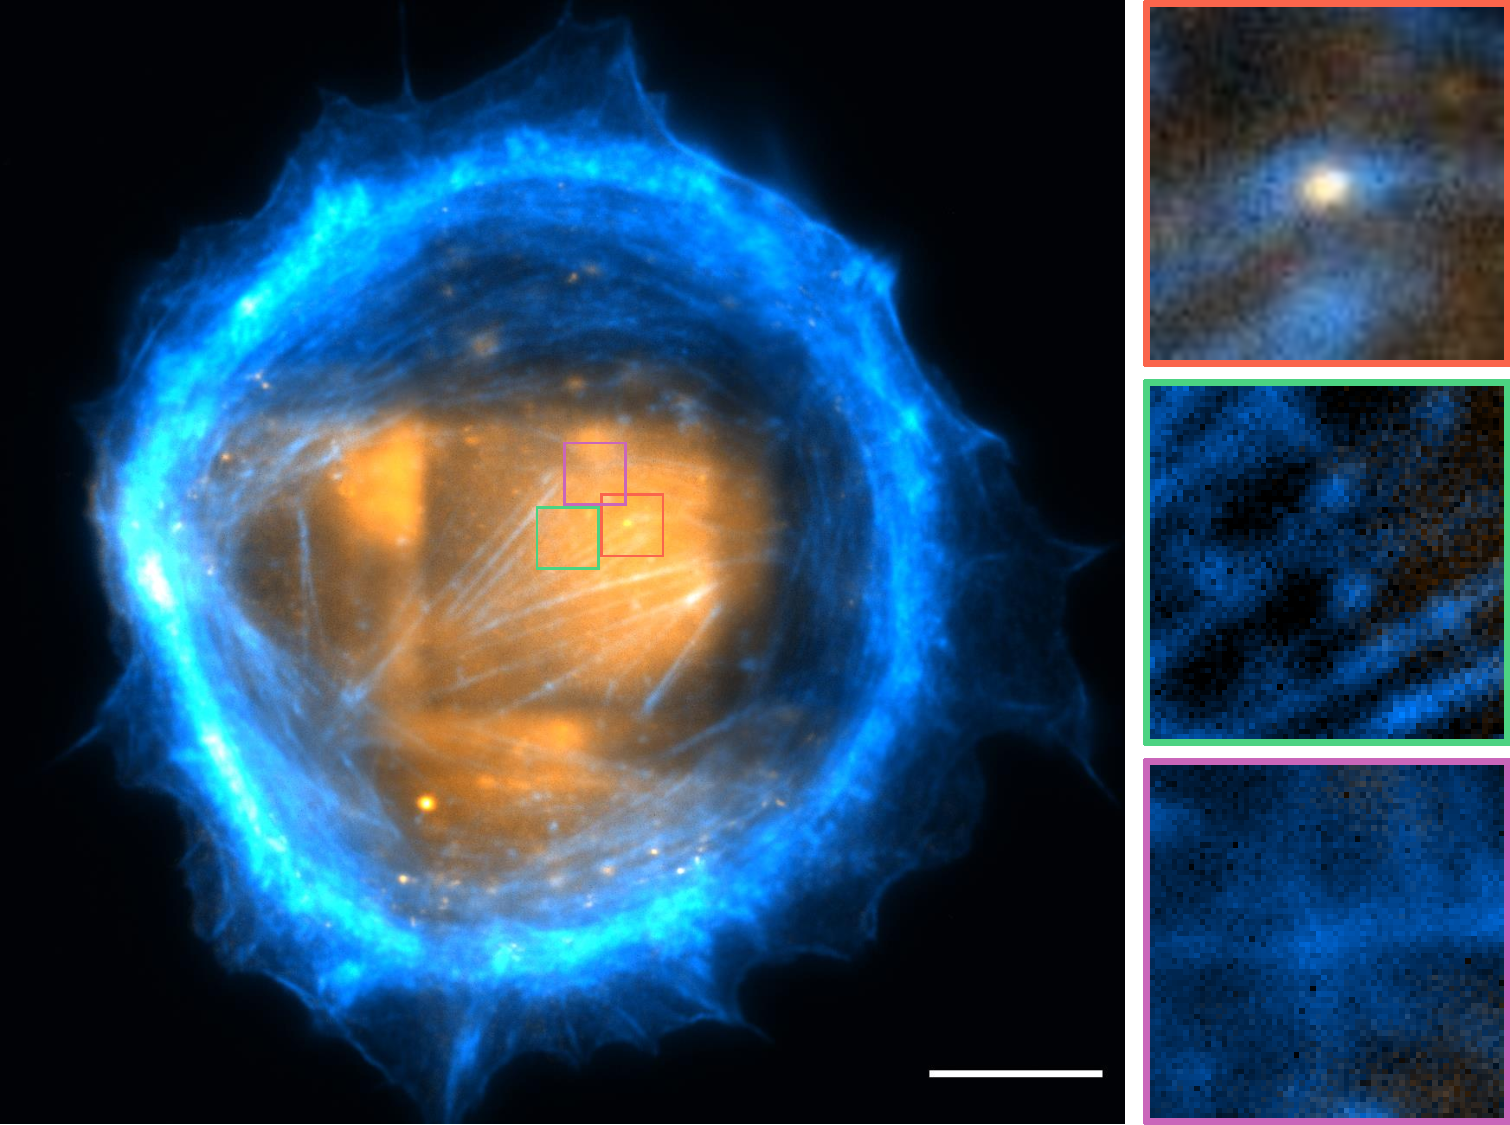
\includegraphics[width=\textwidth]{actin-kras-wf}
	\caption{}\label{fig:widefield-actin}
\end{subfigure}

~\newline
\begin{subfigure}[b]{0.85\textwidth}
	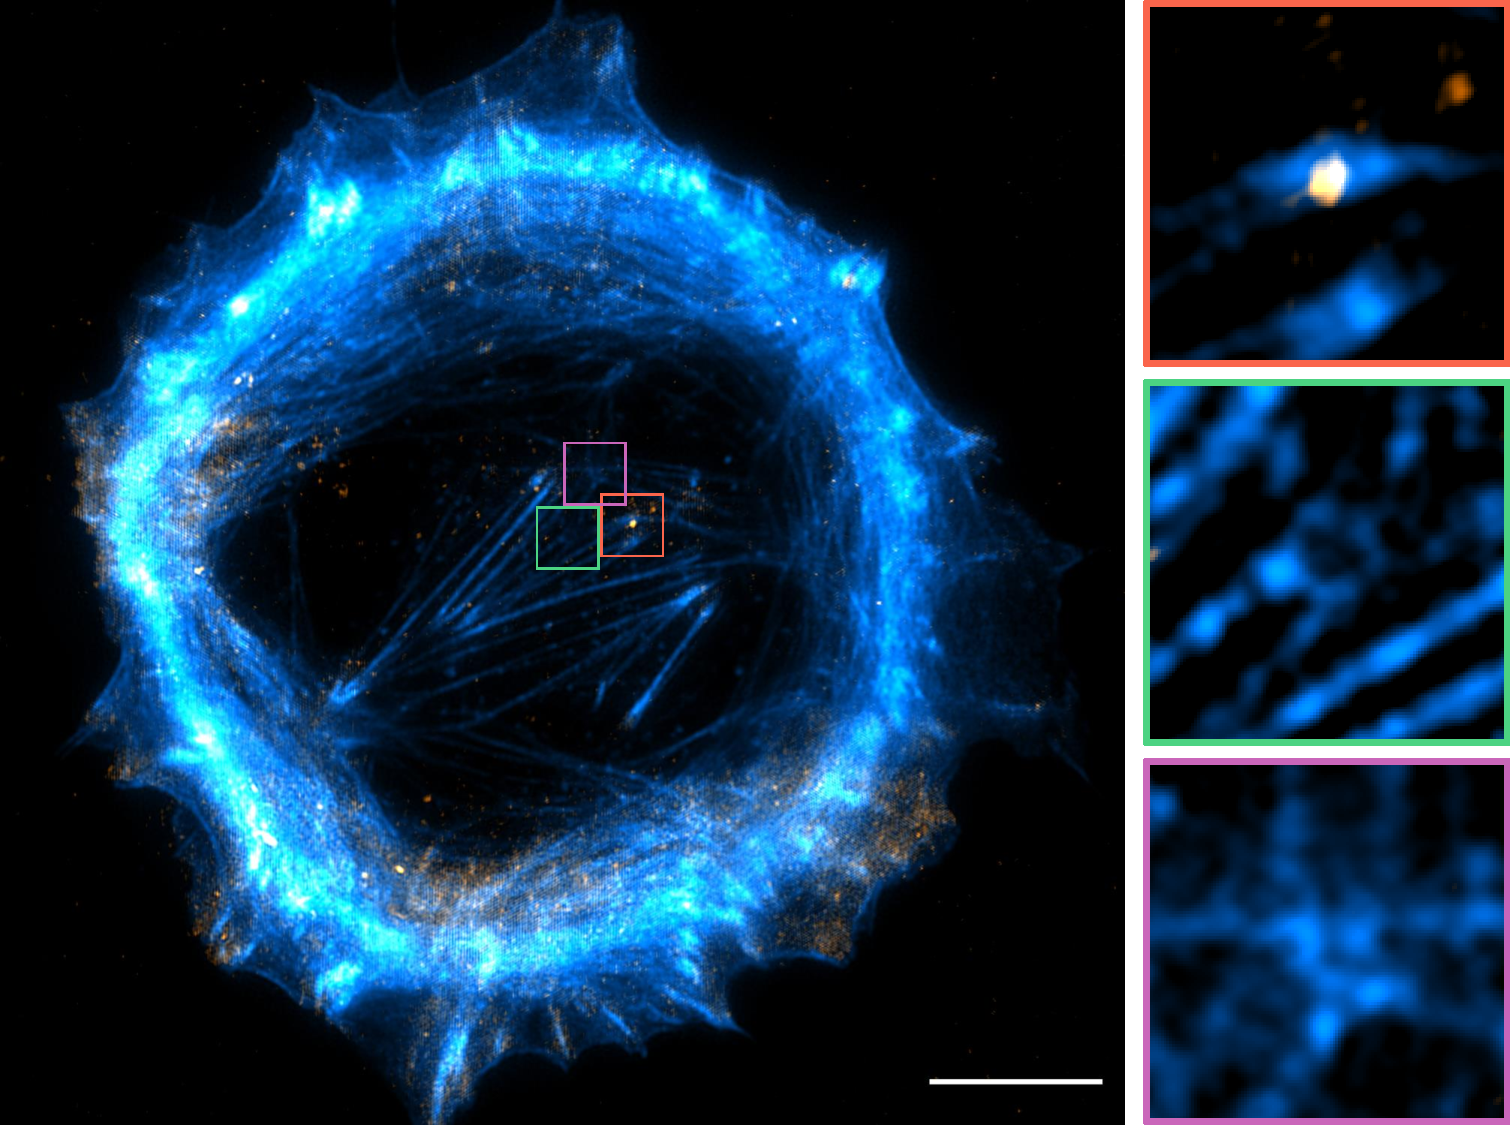
\includegraphics[width=\textwidth]{actin-kras-sim}
	\caption{}\label{fig:recon-tirf-actin}
\end{subfigure}
\caption[LAG SIM: TIRF-SIM imaging of actin in MEF cells removes out-of-focus light allowing actin development to be studied]{(a) shows actin labelled in MEF cells, where out-of-focus light blurs details in the actin. Utilising TIRF-SIM, shown in (b), enhances resolution and removes out-of-focus light. Inset images show various stages of actin development, with a dense cluster of actin (inset in red box) forming into a ring structure (inset in green box) which acts as a source for new filament growth (inset in purple box). Cells were prepared for imaging by Anchal Chandra. Scalebars are \SI{10}{\micro\metre} long, and inset images are \SI{3.2}{\micro\metre} squares.}
\label{fig:recon-actin}
\end{figure}
\afterpage{\clearpage}

A reconstructed TIRF-SIM image is shown in Figure~\ref{fig:recon-tirf-actin}.
In contrast to the widefield image, individual clusters of protein can now be clearly identified, with the out-of-focus background light removed.
Furthermore, the structure of individual actin filaments can now be clearly resolved.

During these experiments 3 distinct phases of actin development were observed, shown in Figure~\ref{fig:recon-tirf-actin}'s coloured boxes.
The red box shows an early stage of development, with KRAS protein colocalised with a dense area of the actin label.
As time progresses, the actin forms a ring structure, seen in the green inset box.
Finally long actin filaments begin to grow out of the ring structure, as shown in the purple box.

Work is currently ongoing to optimise the labelling of the KRAS protein.
Under the current labelling scheme only one frame of the \SI{488}{\nano\metre} channel could be captured before photobleaching of the fluorescent label reduced the signal-to-noise ratio so that artefact-free SIM reconstruction could no longer be performed.
Various fluorescent probes are now under investigation to design a scheme where the KRAS protein can be imaged for the full time-lapse duration.
It is hypothesised that KRAS protein will be colocalised with the ring structure as it forms and as the actin filaments grow from it.
LAG SIM's unique combination of high-speed, high resolution, multicolour TIRF imaging make it one of the only instruments in the world that can capture these events to test the hypothesis.


\subsection[Resolution-enhanced optical sectioning of brain-slice tissue imaging for measuring the Node of Ranvier]{Resolution-enhanced optical sectioning of brain-slice tissue\\ imaging for measuring the Node of Ranvier}
Neurons in the brain communicate at junctions known as synapses, which are formed where an axon from one neuron meets a dendrite from another~\cite{hall1992introduction}.
The axons, coloured yellow in Figure~\ref{fig:neuron-diagram}, form long, thin projections, and can be compared to electrical wires carrying signals across the brain to control bodily functions such as sensing, movement, and conciousness.

Figure~\ref{fig:neuron-diagram} shows axons coated in a fatty sheath known as myelin~\cite{hall1992introduction}.
This protects the axon from interference with other nearby axons, and increases the transmission speed of electrical signals as action potentials jump from one gap in the myelin sheath - known as a Node of Ranvier - to the next in a process called saltatory conduction~\cite{tasaki1939electro}.
Diseases which cause injury to the myelin sheath are associated with motor neuron disorders such as multiple sclerosis and leukodystrophy~\cite{suzuki2001demyelinating}.

\begin{figure}[htbp!]
\centering
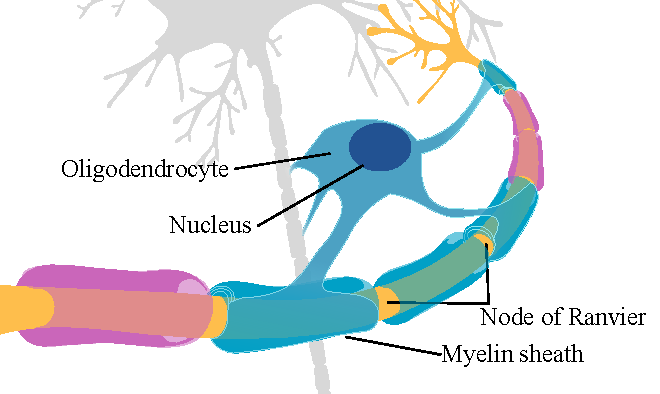
\includegraphics[width=1.0\textwidth]{neuron-diagram}
\caption[LAG SIM: Diagram of a neuron showing an axon protected by the myelin sheath]{Diagram of a neuron, adapted from Wikipedia~\cite{wikineuron}. A neuron, coloured in yellow, has long wire-like projections called axons. Axons are covered by a fatty coating known as the myelin sheath, which protects it from interference from neighbouring axons and increases the transmission speed of signals. The myelin sheath is part of a different brain cell type called an oligodendrocyte, shown here in blue. The gap between two myelin sheaths is known as the Node of Ranvier. }
\label{fig:neuron-diagram}
\end{figure}
\afterpage{\clearpage}

The myelin sheath is not part of the neuron cell, but is rather a component of another type of brain cell called an oligodendrocyte, shown in blue in Figure~\ref{fig:neuron-diagram}~\cite{hammond2012cellular}.
Oligodendrocytes are created from cell-linage parent cells called oligodendrocyte progenitor cells (OPCs), which themselves are derived from embryonic stem cells~\cite{goldman2015make}.
In mouse models two developmentally distinct OPC populations exist: a first wave of OPCs arise from precursors in the ventral part of the brain at day 15 of embryo development; then a second wave of OPCs from dorsal precursors develop from birth~\cite{kessaris2006competing}.
Collaborators have shown that when one of these waves of OPCs is genetically suppressed mice are still able to develop to maturity, but have significant difficulties with fine motor control.

It was hypothesised that a physiological difference in the myelin sheath would be visible between oligodendrocytes derived from ventral OPCs and those derived from dorsal OPCs.

A fluorescent labelling scheme was devised by collaborators to distinguish between ventrally- and dorsally-derived oligodendrocytes.
Also, the Node of Ranvier was made visible by labelling the end of myelin sheaths in a third colour; the distance between two adjacent labels was therefore the length of the Node of Ranvier.
The collaborators were interested to find whether there was a difference in this length for the two oligodendrocyte lineages.

The SIM examples presented in this results section so far have shown data of cultured cells which form a single layer on the microscope slide, and do not stack on top of each other.
However, the versatility of LAG SIM also allows it to perform tissue imaging beyond the diffraction limit.

Imaging deep in tissue is a notorious challenge in microscopy for two main reasons~\cite{wimmer2010high}.
Firstly, multiple layers of fluorescent cells cause significant out-of-focus light, which obscures details in the focal plane.
Secondly, scattering of photons as the light passes through multiple refractive index changes means that it becomes more and more difficult to focus light the deeper into the tissue one tries to observe~\cite{jacques2013optical}.
Both these issues are particularly problematic in SIM, as the out-of-focus light degrades the modulation contrast of the sinusoidal illumination pattern, and scattering of photons as they travel to the focal plane leads to less pattern-generating interference, as shown in Figure~\ref{fig:tissue-illumination}.

\begin{figure}[htbp!]
\centering
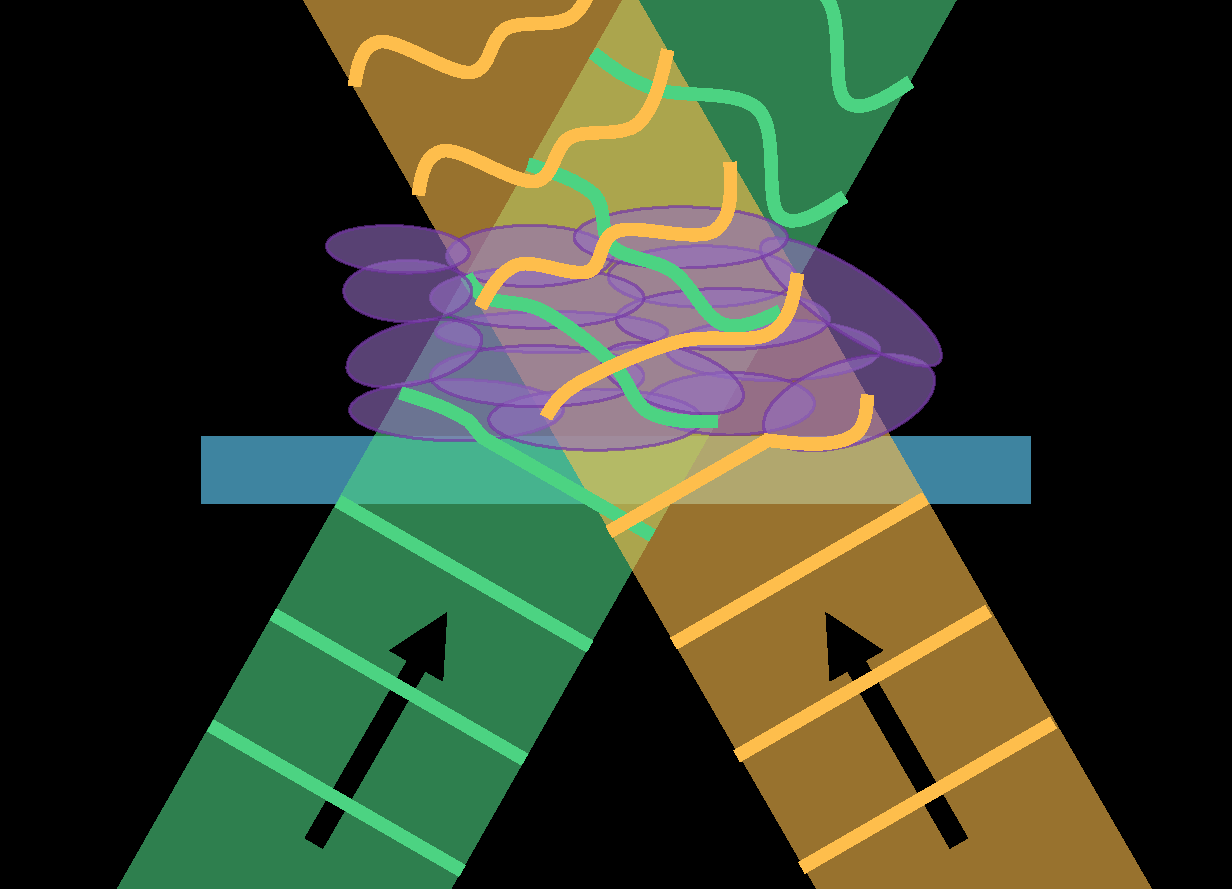
\includegraphics[width=1.0\textwidth]{tissue-illumination}
\caption[LAG SIM: Imaging in tissue degrades the SIM pattern due to photon scattering and out-of-focus light]{A false-colour diagram of SIM imaging in thick tissue samples.
As light passes through tissue, scattering of photons causes the wavefront to become distorted. When the two beams meet at the focal plane, distortion of the wavefronts means that the sinusoidal interference pattern is degraded. Moreover, out-of-focus light from fluorescence above and below the focal plane further reduces the modulation contrast of the interference pattern. Due to these effects, LAG SIM can only produce reliable images about \SI{10}{\micro\metre} into thick samples. Note that the diagram is not to scale, and that the green and yellow beams come from the same laser source but false-colour has been used for clarity. }
\label{fig:tissue-illumination}
\end{figure}

Nevertheless, it has been found that LAG SIM can image up to \SI{10}{\micro\metre} into tissue without degradation of the reconstructed images.

\SI{8}{\micro\metre}-thin slices of mouse brain were labelled to study the myelin sheath of oligodendrocytes.
Myelin was labelled in one of two colours, depending on whether the cell originated from the ventral or dorsal area of the brain.
The end of each myelin sheath was labelled with a third colour to measure the length of the Node of Ranvier, to discover whether there is an observable difference between the two oligodendrocyte types related to disease pathology.

To allow the greatest imaging depth, the lens with the closest refractive index matched to the tissue was chosen; in this case, the 60$\times$ water lens.
A greater penetration depth could be achieved with a lens better matched to the tissue's refractive index, for example a silicon-oil immersion lens with a refractive index of \num{1.406}, if one is available.
A z-stack was captured with a step-size of \SI{0.2}{\micro\metre}, to build up a 3D image.
Cells were fixed, so a raw frame exposure time of \SI{200}{\milli\second} was used to ensure a high signal-to-noise ratio.

To remove out-of-focus light in the reconstructed SIM images, OTF attenuation was used in the LAG SIM Fiji plugin.
An attenuation FWHM of 1.2 and an attenuation strength of 0.995 were chosen, which Section~\ref{sec:LAGSIM-OTF-attenuation} shows provide optical sectioning without introducing artefacts.
Richardson-Lucy filtering was applied to the input images to suppress noise, and a Wiener parameter of 0.1 was chosen for output filtering.
Table~\ref{tab:resolution} shows that the resolution enhancement provided by the 60$\times$ lens in optical sectioning mode is 1.59 to 1.67 - however, relatively weak pattern modulation contrast lead to high-frequency artefacts in reconstructed images, so an apodisation cutoff of 1.5 was chosen to suppress artefacts as much as possible, with an attenuation strength of 0.8 to approximate the shape of a widefield OTF.

The reconstruction parameters entered into the LAG SIM Fiji plugin are summarised as follows:\newline
\begin{tabular}{p{0.5\textwidth}p{0.5\textwidth}}
\begin{labelling}[margin={Attenuation strength}]
	\item[Filter] RL in, Wiener out
	\item[Wiener parameter] 0.1
	\item[Apodiation cutoff] 1.5
	\item[Apodiation strength] 0.8
\end{labelling} &
\begin{labelling}[margin={Attenuation strength}]
	\item[RL steps] 5
	\item[OTF attenuation] true
	\item[Attenuation FWHM] 1.2
	\item[Attenuation strength] 0.995
\end{labelling}
\end{tabular}

\begin{figure}[tbp!]
\centering
\includegraphics[width=1.0\textwidth]{recon-brain}
\caption[LAG SIM: Multicolour optical sectioning SIM to measure the Node of Ranvier on ventrally- and dorsally-derived oligodendrocytes]{Dorsally-derived and ventrally-derived oligodendrocytes are coloured in magenta and cyan respectively. The end of the myelin sheath is coloured in orange, and can be used to measure the length of the Node of Ranvier. Optical sectioning SIM was used on \SI{8}{\micro\metre} brain slices. Slices were dissected and labelled by Sarah F{\"o}rster. Scalebar is \SI{10}{\micro\metre}. }
\label{fig:recon-brain}
\end{figure}
\afterpage{\clearpage}

Figure~\ref{fig:recon-brain} shows a slice of a reconstructed z-stack.
Orange dots marking the ends of myelin sheaths are located either on dorsally-derived oligodendrocytes, shown in magenta, or on ventrally-derived oligodendrocytes, shown in cyan.
The length of the Node of Ranvier is measured as the distance between two adjacent orange markers.
Lengths were measured automatically with a custom script in the image analysis suite Icy~\cite{de2012icy}, and assigned to ``dorsally-derived'' or ``ventrally-derived'' based on the colour of the oligodendrocyte they were located on.

The signal-to-noise ratio in the reconstructed images is notably poor for the oligodendrocyte channels, and artefacts have been introduced by the SIM algorithm despite optimal reconstruction parameters.
This can be explained by a high 3D density of oligodendrocytes, causing lots of out-of-focus light in the focal plane which reduces the modulation contrast of the SIM illumination pattern.
As derived in Section~\ref{sec:SIM-theory}, pattern contrast is directly proportional to signal-to-noise ratio for the high-frequency components in reconstructed SIM images, so excessive background light severely affects the ability to produce clear SIM images.

In contrast to the oligodendrocyte channel, the orange Node of Ranvier channel has a low density of fluorescent markers.
The SIM pattern modulation contrast is therefore not degraded by out-of-focus light, leading to artefact-free SIM reconstructions with a high signal-to-noise ratio.
This allows accurate length measurements of the Node of Ranvier.
Since length was the important measurement for this experiment, and the oligodendrocyte type could still be determined despite the substandard reconstruction, the images were sufficient for testing the hypothesis that dorsally-derived oligodendrocytes have a different Node of Ranvier length from ventrally-derived oligodendrocytes.

Upon analysis of the data a statistically-significant difference was not calculated, suggesting that there is no difference in the Node of Ranvier length between the two oligodendrocyte types and that the movement problems observed at the organism level must arise from another characteristic of the cells, or a more complicated combination of properties.
Nevertheless, this experiment has shown the versatility of the LAG SIM instrument and its ability to image tissue samples as well as cultured cells.

\section{Conclusion}
LAG SIM has been restored to its fast imaging speed of 11 super-resolution frames per second through the introduction of a Pockels cell for polarisation rotation.
The Pockels cell is a robust, future-proof solution to ensure that the SIM illumination is generated with high pattern contrast.
With this successfully in place, the other desirable features for LAG SIM could be addressed.

The instrument can now quickly switch between TIRF imaging, resolution-enhanced SIM imaging and SIM optimised for optical sectioning using user-friendly software which interacts seamlessly with the new hardware.
This makes it suited to a wide variety of biological imaging experiments, as presented in Section~\ref{sec:sim-showcase}.

The addition of an Optosplit, made possible by the implementation of the Pockels cell in lieu of an LCVR, further enhances LAG SIM's fast imaging capability.
Rather than requiring the use of a filter wheel to switch between colour channels, 3 colours can be imaged simultaneously.
This removes any mechanical movement from the system, reducing the fastest 3-channel acquisition from \SI{570}{\milli\second} to the headline \SI{90}{\milli\second}, a 5-fold improvement in frame rate.

Considerable care has been taken to ensure the microscope can be operated by non-expert users.
The interface is clear and compact, and can be taught to new users in a single imaging session.
This means that LAG SIM can be used unsupervised, saving time and allowing for the microscope to perform a diverse range of world-leading biological research.

Finally, the LAG SIM Fiji plugin complements the easy-to-use microscope to help users generate artefact-free images.
As shown throughout this chapter, reconstruction is a complicated process involving complex mathematics and optical engineering.
LAG SIM simplifies this process, so that a user can go from hypothesis to result without the need for a full-time SIM expert.

In addition to the biological investigations presented here, Chapters~\ref{chap:MOF} and \ref{chap:ER} describe in detail two successful experiments facilitated by LAG SIM.
Before that, however, Chapter~\ref{chap:FPB} reveals FPBioimage, a user-friendly tool for visualising and sharing 3D volumetric data, such as those obtained through optical sectioning on the LAG SIM.
